\section{Design}
\subsection{Metodologie di Sviluppo}

Il team ha adottato un approccio ispirato a \textbf{SCRUM} per il processo di sviluppo,
che comprende la creazione iniziale del backlog del prodotto e la pianificazione
del primo sprint durante un incontro iniziale.\\
Gli sprint sono stati strutturati con una durata settimanale al fine di ottenere
risultati concreti e di valore per gli stakeholder.\\ Sono stati condotti frequenti
incontri all'inizio e alla fine di ciascuno sprint, mantenendo un backlog dello sprint
per tenere traccia dell'organizzazione del lavoro.\\
Il primo sprint si è concentrato sull'analisi del settore, inclusa la conduzione di
interviste simulate con il committente e la creazione di tutti gli artefatti necessari
per l'analisi del dominio.\\ Inoltre, in questo primo sprint abbiamo definito gli strumenti
DevOps e impostato l'infrastruttura per la build automation, continuous integration
e il versioning control, per poterne beneficiare fin da subito.\\ Questo sprint iniziale
è stato di fondamentale importanza per il progetto ed è stato svolto in modo collaborativo
da tutti i membri del gruppo.\\
Successivamente, il team ha deciso di suddividere il lavoro in quattro sprint aggiuntivi:

\begin{itemize}
    \item \textbf{Sprint 2-3}: dedicati alla creazione e testing dei microservizi (con relativa gestione della consistenza dei dati attraverso MongoDB) per ciascun bounded context che era stato identificato con un focus sulle relative API RestFul;
    \item \textbf{Sprint 4-5}: dedicati alla creazione e testing di una webApp per la gestione dell’interfaccia utente;
    \item \textbf{Sprint 6-7}: dedicati alla rimodellazione e ristrutturazione del codice Client con i relativi test nonché alla stesura stessa di questa relazione.
\end{itemize}

In totale, sono stati completati sette sprint nel corso del processo di sviluppo del progetto.\vspace{3mm}

Parallelamente al processo di sviluppo, è stata adottata una metodologia di design chiamata \textbf{UCD (User Centered Design)}.\\
La scelta di questa metodologia è stata determinata dal fatto che, fin dalle prime fasi di progettazione,
si è voluto dare priorità alla \textbf{HCI (Human Computer Interaction)}, concentrando l’attenzione sulle necessità
degli utenti e sull’obiettivo di garantire un’usabilità ottimale per migliorare l’esperienza dell’utente.\\
Per quanto riguarda l’implementazione dell’applicazione, il focus si è posto sul dover soddisfare le esigenze e le richieste degli utenti.\\
Gli User a cui si farà riferimento successivamente sono rappresentati attraverso una serie di profili chiamati “personas”, che riflettono un possibile pubblico di riferimento dell’applicazione.
\newpage
\subsection{Target User Analysis}

Nel contesto della gestione di un magazzino alimentare, sia gli utenti amministrativi che operativi si
trovano a dover affrontare una serie di compiti complessi e cruciali.\\ Gli utenti amministrativi sono responsabili
della supervisione generale delle operazioni, del monitoraggio delle scorte, della gestione degli ordini e della
garanzia della qualità e sicurezza degli articoli.\\ Dall' parte, gli utenti operativi sono responsabili dell’esecuzione delle attività quotidiane, come il carico e lo scarico delle merci.

\subsubsection{Descrizione del Target di Utenti}

L'applicazione che intendiamo sviluppare fornirà funzionalità specifiche per entrambi i tipi di utenti.\\
Per gli utenti amministrativi, l’applicazione offrirà una dashboard centralizzata che fornirà informazioni
dettagliate sullo stato degli ordini, dei task e il monitoraggio delle temperature nelle zone refrigerate.\\
Inoltre, attraverso notifiche proattive, gli utenti amministrativi saranno avvisati tempestivamente di situazioni
critiche come deviazioni di temperatura o scorte a rischio di esaurimento. Per gli utenti operativi, l’applicazione
semplificherà notevolmente le operazioni quotidiane. Una funzionalità chiave sarà la possibilità di eseguire facilmente
compiti come il carico e lo scarico delle merci attraverso un’interfaccia intuitiva e user-friendly.\\
Inoltre, l’applicazione fornirà agli utenti operativi istruzioni dettagliate e supporto in tempo reale per garantire l’esecuzione corretta delle attività.

\subsubsection{Analisi Strategica per la Realizzazione dell'Applicativo}

Per soddisfare pienamente i requisiti degli utenti, sono state effettuate delle analisi strategiche:

\begin{itemize}
    \item \textbf{Conoscenza dei Compiti Utente}: Comprendere le procedure necessarie per la gestione di un magazzino alimentare, inclusi i passaggi che un utente amministrativo deve compiere per monitorare e gestire le scorte e gli ordini, e le azioni che un utente operativo deve eseguire quotidianamente.
    \item \textbf{Ottimizzazione dell’Applicativo}: Il servizio deve essere intuitivo, poiché gli utenti operativi e amministrativi potrebbero non avere familiarità con strumenti digitali avanzati. La semplicità e l'intuitività nell'uso delle varie funzionalità renderanno l'uso del servizio più appagante.
    \item \textbf{Affidabilità e Prestazioni}: Gli utenti si aspettano che l'applicativo funzioni come supporto affidabile per la gestione del magazzino. Di conseguenza, l’applicazione non deve presentare anomalie progettuali o funzionali che possano compromettere l’efficienza operativa.
\end{itemize}

\subsubsection{Categorie di Utenti}

Il target di utenza è suddiviso in due categorie principali:

\begin{itemize}
    \item \textbf{Utenti Amministrativi}: Responsabili della supervisione generale del magazzino, monitoraggio delle scorte, gestione degli ordini e garanzia della qualità e sicurezza degli articoli. Hanno bisogno di strumenti di gestione avanzati, dashboard centralizzate e notifiche proattive per gestire situazioni critiche.
    \item \textbf{Utenti Operativi}: Responsabili delle operazioni quotidiane nel magazzino, come carico e scarico delle merci e mantenimento dell'ordine. Necessitano di un’interfaccia user-friendly, istruzioni dettagliate e supporto per eseguire le loro attività in modo efficiente.
\end{itemize}

\subsubsection{Personas}

Di seguito vengono riportati diversi personas, rappresentazioni ipotetiche di utenti che devono utilizzare l’applicativo per assolvere determinati compiti.

\textbf{Persona: Mario, 45 anni, Responsabile del Magazzino}

\textbf{Scenario d’uso}: Mario è il responsabile del magazzino alimentare.\\
Ha un'esperienza di oltre 20 anni nel settore e si occupa principalmente della supervisione delle operazioni,
del monitoraggio delle scorte, della gestione degli ordini e della gestione degli utenti.

\begin{itemize}
    \item Mario accede al sito effettuando il login con le sue credenziali amministrative o si registra se è il suo primo accesso.
    \item Utilizza la dashboard per monitorare lo stato del magazzino, inclusi lo stato degli ordini, task e temperatura delle varie zone.
    \item Riceve notifiche proattive riguardanti deviazioni di temperatura e scorte a rischio di esaurimento.
    \item Gestisce gli ordini e monitora la quantità degli articoli stoccati.
    \item Gestite i task da assegnare agli utenti operativi.
    \item Gestisce le informazioni relative agli utenti.
\end{itemize}

\textbf{Persona: Luca, 30 anni, Operatore di Magazzino}

\textbf{Scenario d’uso}: Luca è un operatore di magazzino che si occupa del carico e dello scarico delle merci.\\È esperto nell'uso di attrezzature per la movimentazione dei materiali e segue rigorosamente le procedure di sicurezza.

\begin{itemize}
    \item Luca accede al sito utilizzando le sue credenziali operative o si registra se è al primo accesso.
    \item Utilizza un’interfaccia intuitiva per registrare l'avanzamento e il completamente dei task per il carico e lo scarico delle merci.
    \item Segue istruzioni dettagliate e riceve supporto per garantire l’esecuzione corretta delle attività.
\end{itemize}

Questi profili aiutano a mantenere il focus sulle esigenze degli utenti durante tutte le fasi di sviluppo e
progettazione dell'applicazione.\\ La metodologia \textbf{UCD (User Centered Design)} e il principio
\textbf{KISS (Keep It Simple, Stupid)} sono stati adottati per garantire che l'applicazione sia facile da usare e
risponda efficacemente alle esigenze degli utenti, migliorando l'efficienza operativa e la soddisfazione generale.

\newpage
\subsection{Mockup iniziali}

Durante lo sviluppo dell'applicazione, particolare attenzione è stata rivolta all'interfaccia utente,
cercando di mantenere uno stile grafico semplice e intuitivo.\\ L'obiettivo principale era permettere agli utenti di
navigare tra le diverse pagine e informazioni in modo rapido e intuitivo.

Nella fase iniziale di progettazione, sono stati creati dei mockup per ottenere una versione preliminare dell'aspetto
grafico dell'applicazione.\\ Questi mockup sono stati utilizzati per visualizzare un insieme di funzionalità che si
ritenevano necessarie per l'applicazione.\\ Grazie a queste interfacce preliminari, è stato possibile raccogliere vari
feedback dagli utenti, permettendo di apportare miglioramenti e ottimizzazioni prima della fase di sviluppo finale.\\
\\In seguito i vari mockup realizzati in fase di progettazione:

\begin{figure}[H]
    \centering
    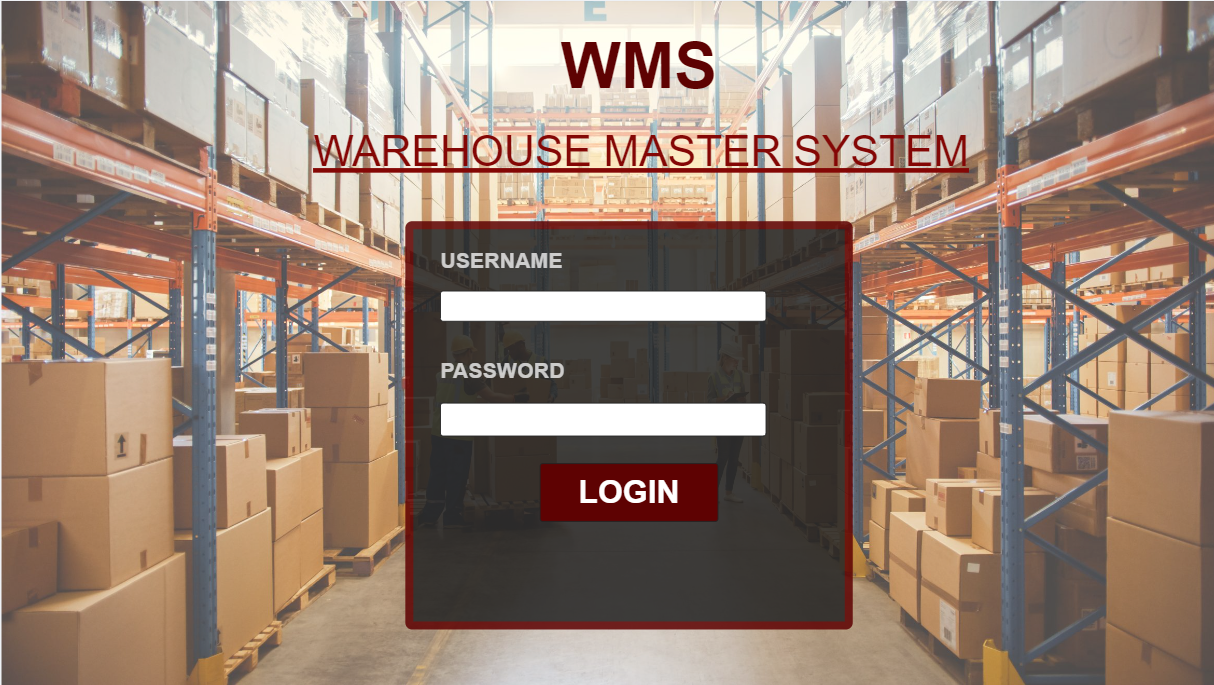
\includegraphics[width=0.8\textwidth]{document/sections/img/login.png}
    \caption{Login Page}
    \label{fig:login}
\end{figure}

L'applicazione si apre con una schermata di login, dove gli utenti possono accedere al sistema utilizzando le loro
credenziali istituzionali.
\newpage
\subsubsection{Admin}

\begin{figure}[H]
    \centering
    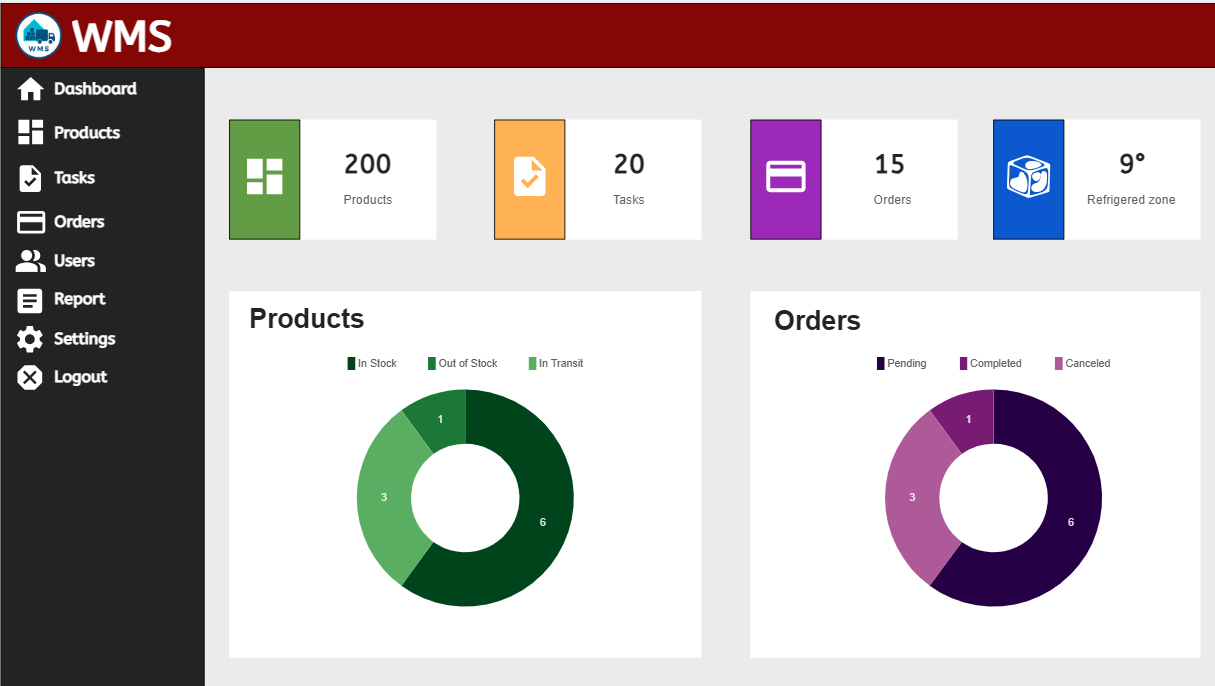
\includegraphics[width=0.8\textwidth]{document/sections/img/homePageAdmin.png}
    \caption{Home Page Admin}
    \label{fig:homePageAdmin}
\end{figure}

Dopo aver completato con successo la fase di autenticazione, l'utente viene reindirizzato alla propria homepage.\\
Questa pagina offre una panoramica intuitiva delle metriche principali per la gestione del magazzino.\\
La homepage è divisa in sezioni chiave.\\ Nella parte superiore, ci sono riquadri colorati che mostrano in tempo reale:
il numero totale di prodotti, compiti, ordini e la temperatura della zona refrigerata.\\
La sidebar a sinistra permette l'accesso rapido alle varie funzionalità dell'applicazione.\\
Ogni sezione è accessibile tramite icone e descrizioni chiare, facilitando la navigazione.\\
Al centro della pagina, sono visualizzati due grafici a torta.\\ Il primo grafico mostra lo stato attuale dei prodotti,
suddiviso in in stock, out of stock e in transito.\\ Il secondo grafico visualizza lo stato degli ordini, distinguendo
tra pendenti, completati e cancellati.\\
L'header della pagina contiene il logo dell'applicazione, posizionato in alto a sinistra.\\
Questo layout garantisce una visione d'insieme delle operazioni del magazzino e un rapido accesso alle funzionalità
necessarie.

\begin{figure}[H]
    \centering
    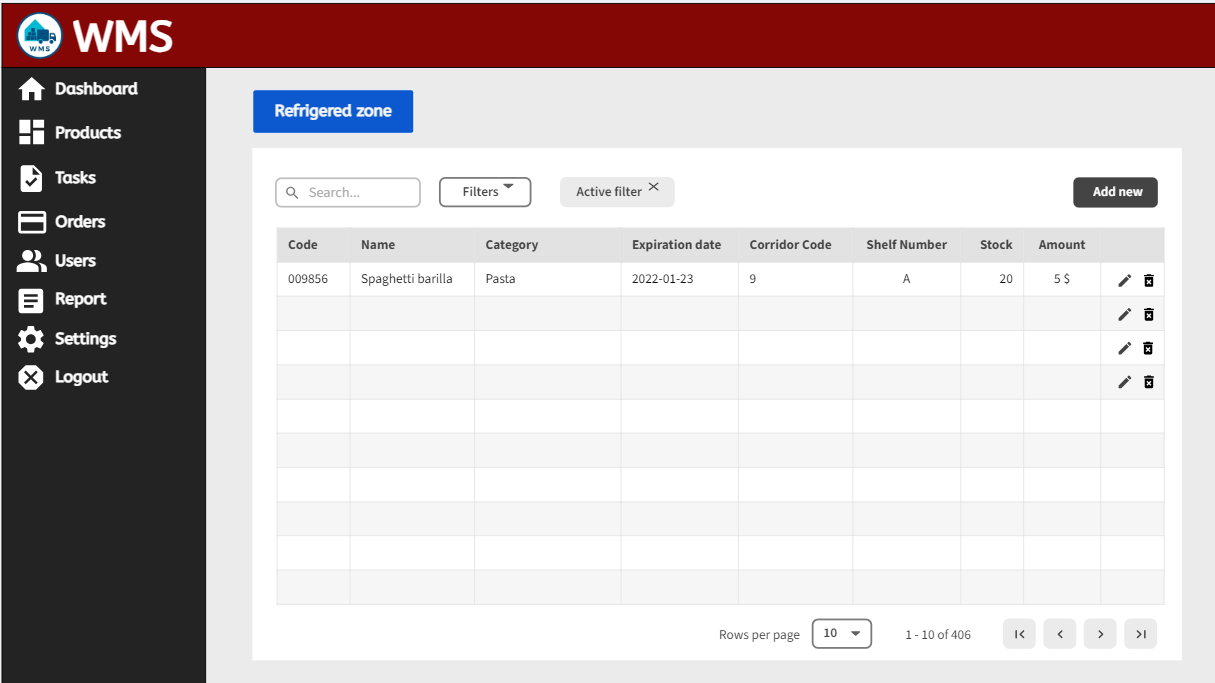
\includegraphics[width=0.8\textwidth]{document/sections/img/productPage.png}
    \caption{Product Page}
    \label{fig:productPage}
\end{figure}

Cliccando sull'icona \textbf{Products} nella sidebar, l'utente viene reindirizzato alla pagina di gestione dei prodotti.\\
Questa pagina offre una visualizzazione tabellare dei prodotti presenti nel magazzino.\\
Nella parte superiore è presente un pulsante \textbf{Add new} che consente di aggiungere nuovi prodotti.

La tabella visualizza informazioni chiave per ogni prodotto e consente di modificarne o eliminarne i dettagli,
cliccando sulle apposite icone nell'ultima colonna a destra della tabella.\\

\begin{figure}[H]
    \centering
    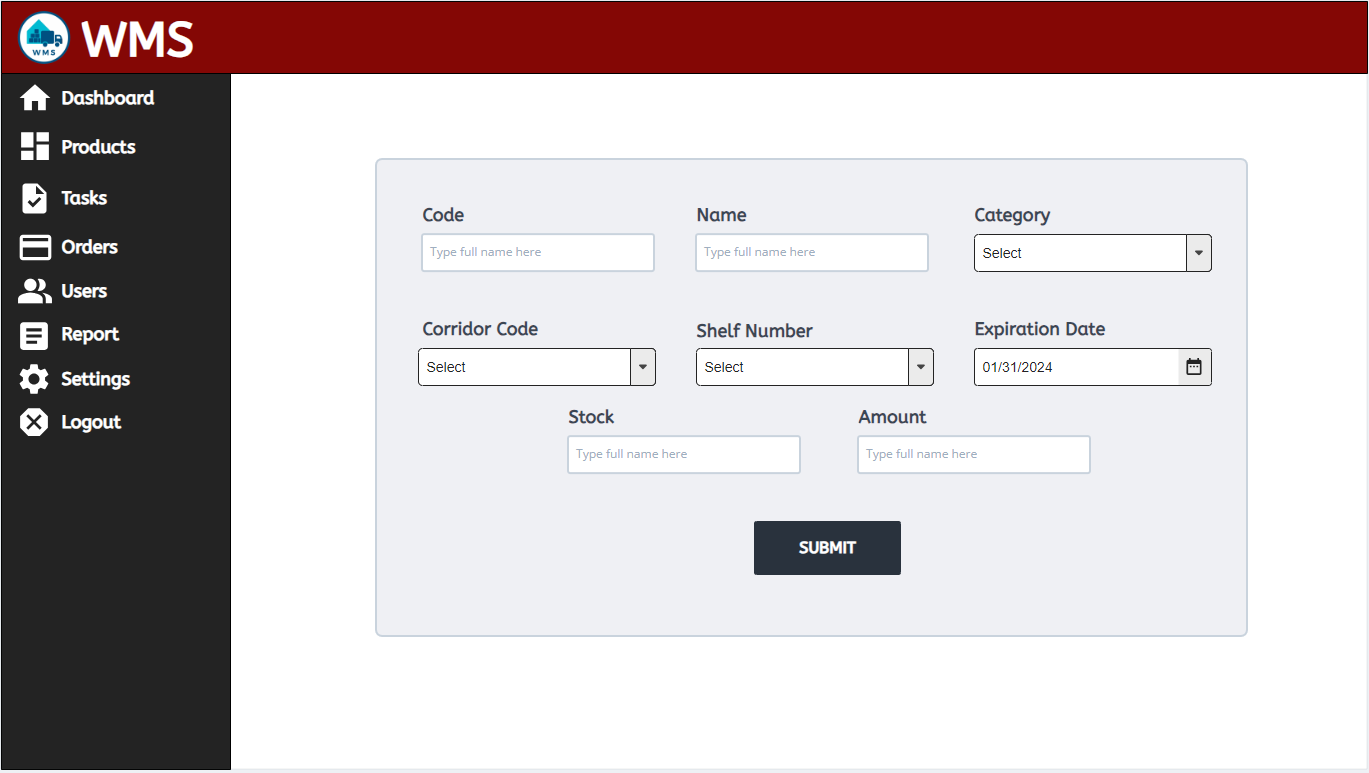
\includegraphics[width=0.8\textwidth]{document/sections/img/AddProduct.png}
    \caption{Add Product Page}
    \label{fig:addProductPage}
\end{figure}
Cliccando sul pulsante \textbf{Add new} nella pagina di gestione dei prodotti,
l'utente viene reindirizzato a questa schermata.
La pagina presenta un modulo di inserimento dati strutturato in modo chiaro e intuitivo,
con tutti i campi necessari per la creazione di un prodotto.


\begin{figure}[H]
    \centering
    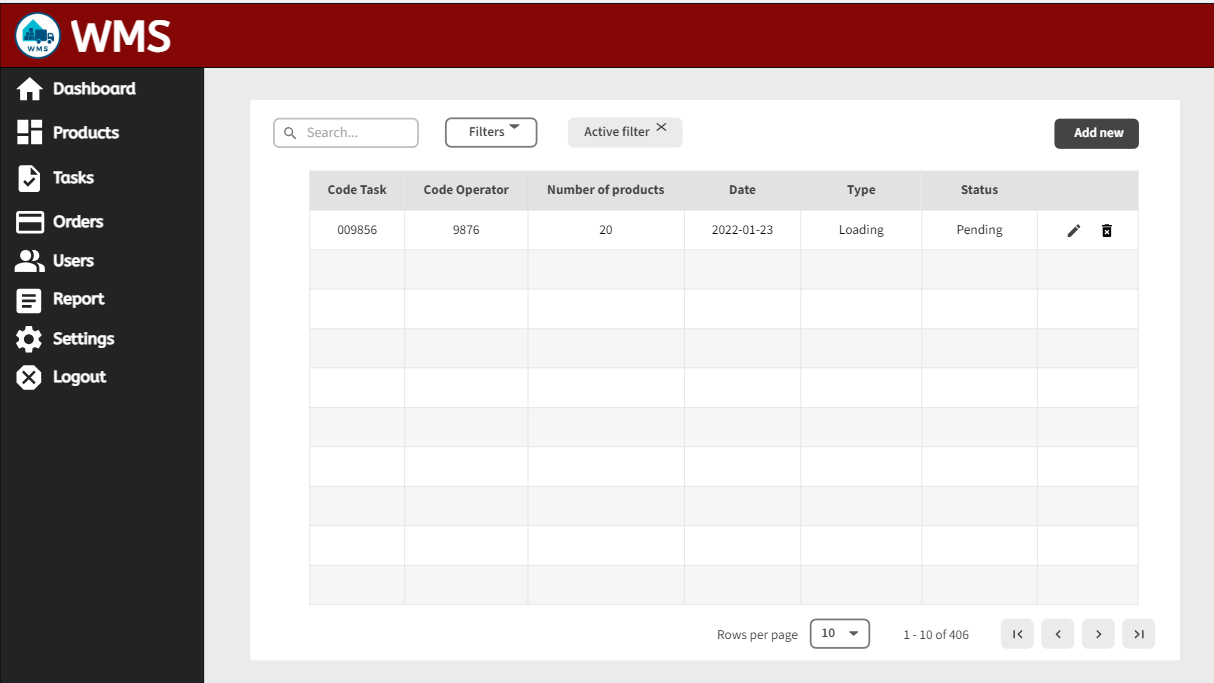
\includegraphics[width=0.8\textwidth]{document/sections/img/taskPage.png}
    \caption{Task Page}
    \label{fig:taskPage}
\end{figure}

Cliccando sull'icona \textbf{Tasks} nella sidebar, l'utente viene reindirizzato alla pagina di gestione dei task.
Questa pagina offre una visualizzazione tabellare dei task presenti nel magazzino.\\
Nella parte superiore è presente un pulsante \textbf{Add new} che consente di aggiungere nuovi task.\\
La tabella visualizza informazioni chiave per ogni task e consente di modificarne o eliminarne i dettagli,
cliccando sulle apposite icone nell'ultima colonna a destra della tabella.

\begin{figure}[H]
    \centering
    \includegraphics[width=0.8\textwidth]{document/sections/img/addTask.png}
    \caption{Add Task Page}
    \label{fig:addTaskPage}
\end{figure}

Cliccando sul pulsante \textbf{Add new} nella pagina di gestione dei task,
l'utente viene diretto a questa schermata.
La pagina mostra un modulo di inserimento dati organizzato in modo chiaro e intuitivo,
contenente tutti i campi necessari per la creazione di un nuovo task.

\begin{figure}[H]
    \centering
    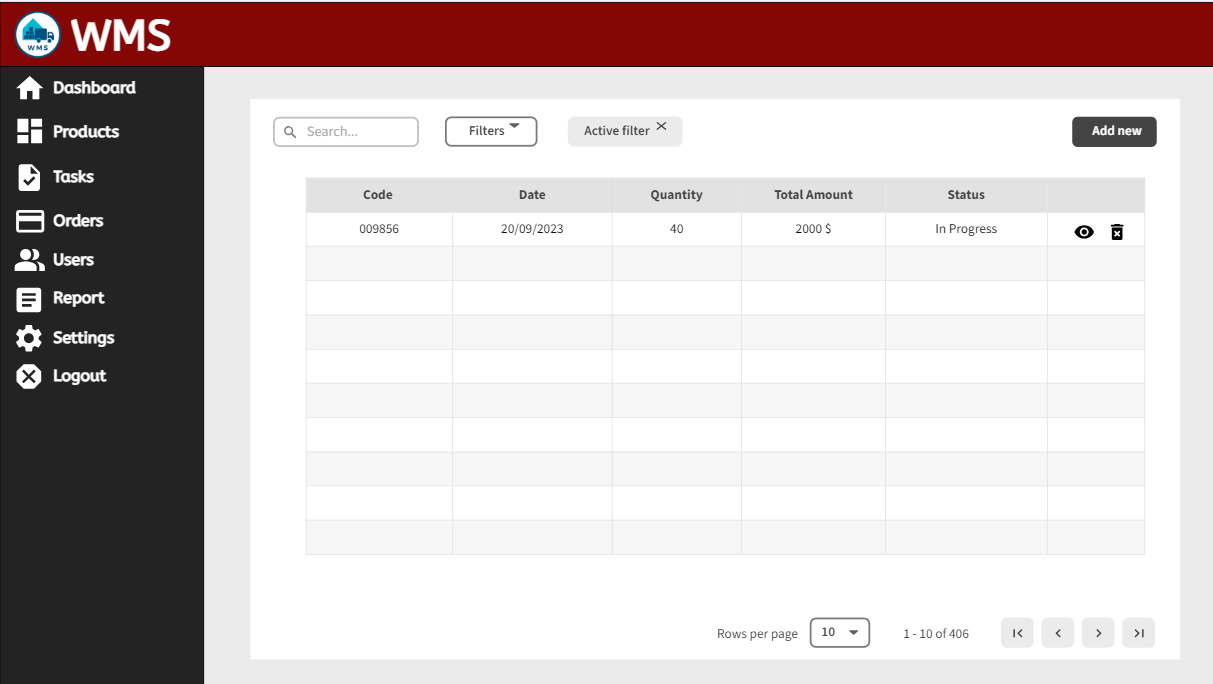
\includegraphics[width=0.8\textwidth]{document/sections/img/orderPage.png}
    \caption{Order Page}
    \label{fig:orderPage}
\end{figure}

Cliccando sull'icona \textbf{Orders} nella sidebar, l'utente viene reindirizzato alla pagina di gestione degli ordini.\\
Questa pagina offre una visualizzazione tabellare degli ordini presenti nel magazzino.\\
Nella parte superiore, è presente un pulsante \textbf{Add new} che consente di aggiungere nuovi ordini.
La tabella visualizza informazioni chiave per ogni ordine e consente di elinarne o visualizzarne meglio i dettagli,
cliccando sulle apposite icone nell'ultima colonna a destra della tabella.

\begin{figure}[H]
    \centering
    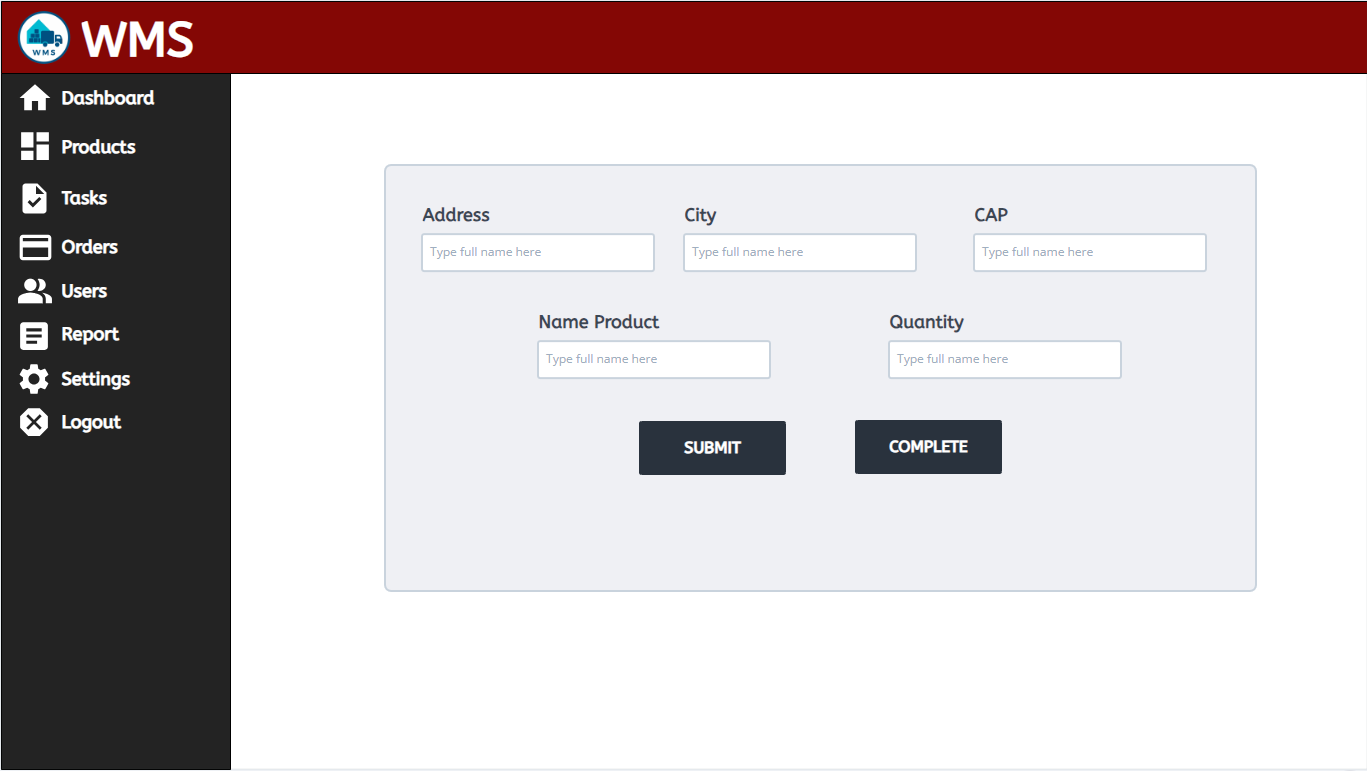
\includegraphics[width=0.8\textwidth]{document/sections/img/AddOrder.png}
    \caption{Add Order Page}
    \label{fig:addOrderPage}
\end{figure}
Cliccando sul pulsante \textbf{Add new} nella pagina di gestione degli ordini,
l'utente viene diretto a questa schermata.
La pagina mostra un form nel quale viene richiesto all'utente di inserire tutti i dati necessari,
per la creazione di un nuovo ordine.

\begin{figure}[H]
    \centering
    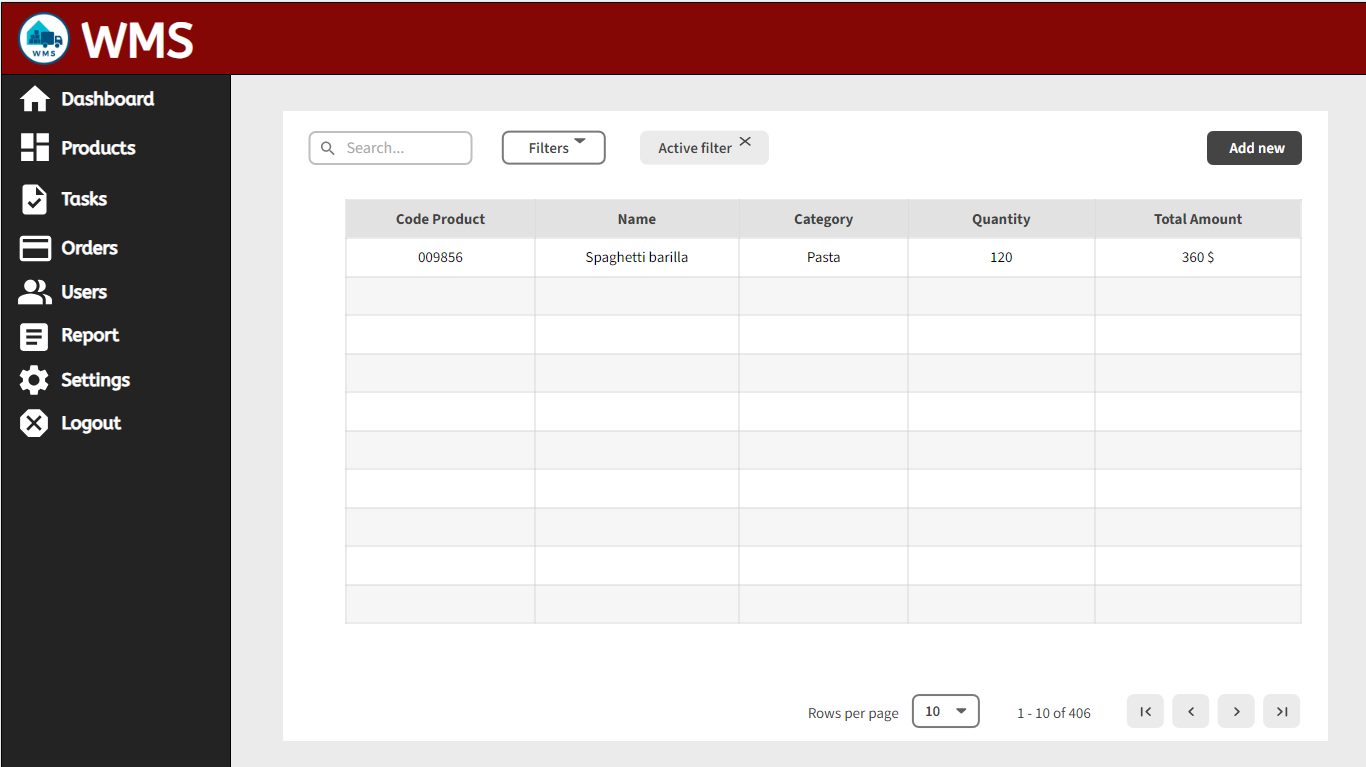
\includegraphics[width=0.8\textwidth]{document/sections/img/OrderView.png}
    \caption{Order View Page}
    \label{fig:orderViewPage}
\end{figure}
Cliccando sull'icona \textbf{View} accanto a un ordine nella pagina di gestione degli ordini,
l'utente viene reindirizzato alla pagina di visualizzazione dei dettagli dell'ordine selezionato.\\
Questa pagina offre una visualizzazione tabellare, mostrando informazioni chiave per ogni prodotto
incluso nell'ordine.

\begin{figure}[H]
    \centering
    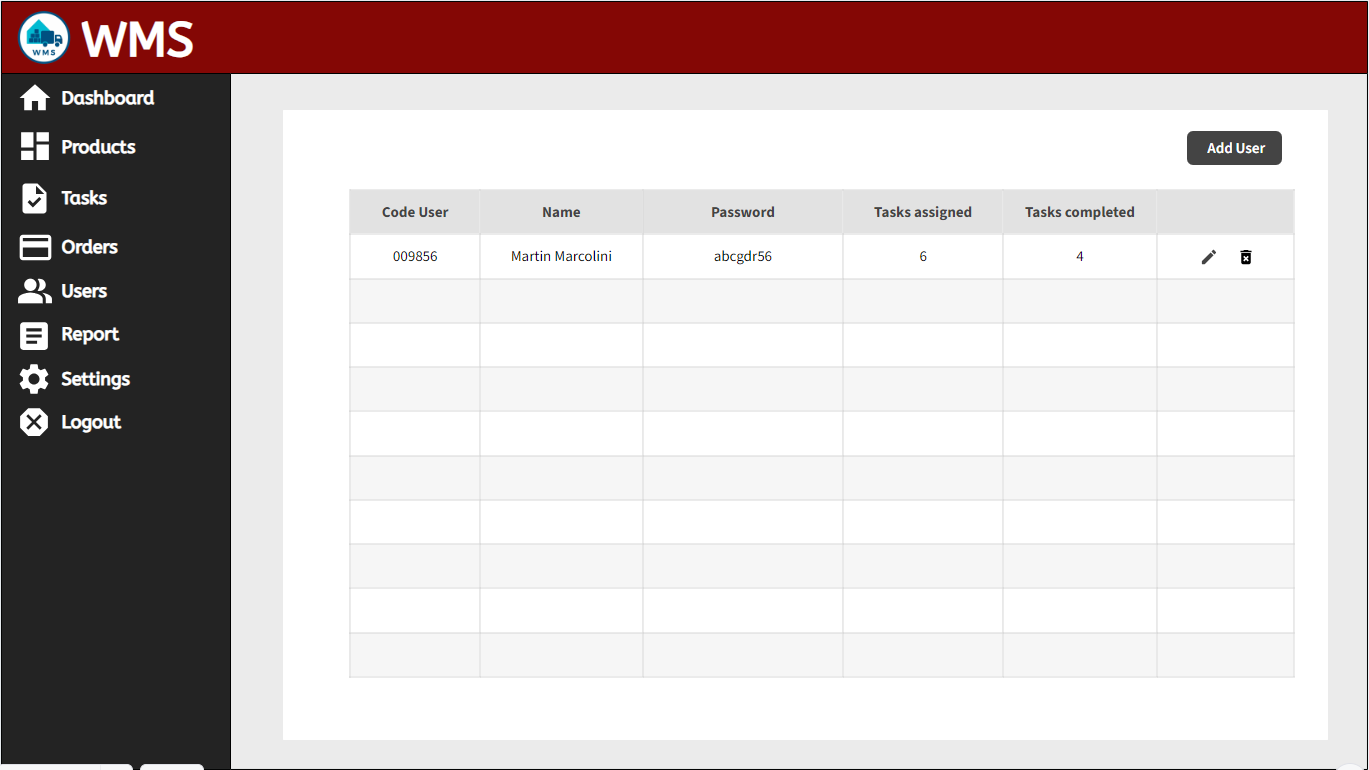
\includegraphics[width=0.8\textwidth]{document/sections/img/UserPage.png}
    \caption{User Page}
    \label{fig:userPage}
\end{figure}
Cliccando sull'icona \textbf{Users} nella sidebar, l'utente viene reindirizzato alla pagina di gestione degli
utenti. Questa pagina offre una visualizzazione tabellare degli utenti presenti nel sistema.\\
Nella parte superiore è presente un pulsante \textbf{Add User} che consente di aggiungere nuovi utenti.\\
La tabella visualizza informazioni chiave per ogni utente e consente di modificarne o eliminarne i dettagli,
cliccando sulle apposite icone.

\begin{figure}[H]
    \centering
    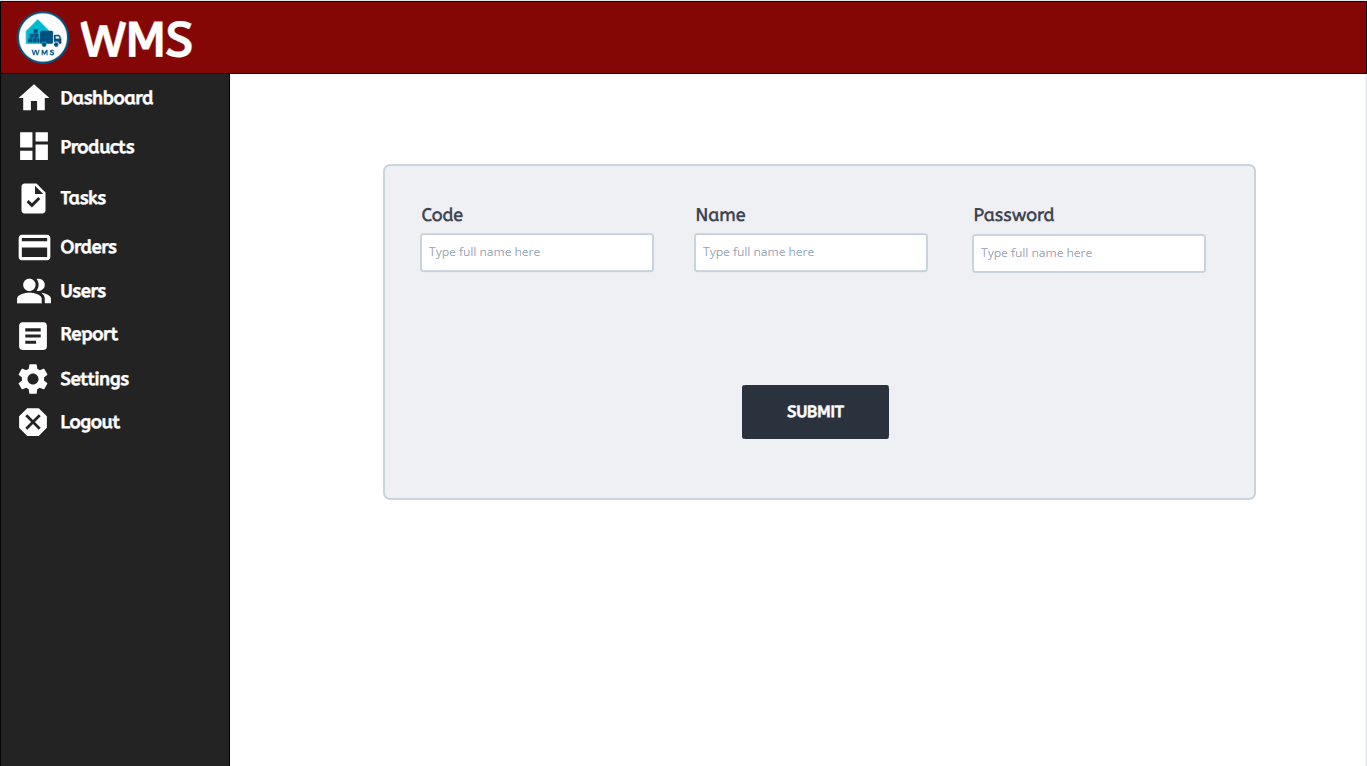
\includegraphics[width=0.8\textwidth]{document/sections/img/AddUser.png}
    \caption{Add User Page}
    \label{fig:addUserPage}
\end{figure}
Cliccando sul pulsante \textbf{Add new} nella pagina di gestione degli utenti,
l'utente viene diretto a questa schermata.
La pagina mostra un form nel quale viene richiesto all'admin di inserire tutti i dati necessari,
per la creazione di un nuovo utente.\\
\subsubsection{Operational}
\begin{figure}[H]
    \centering
    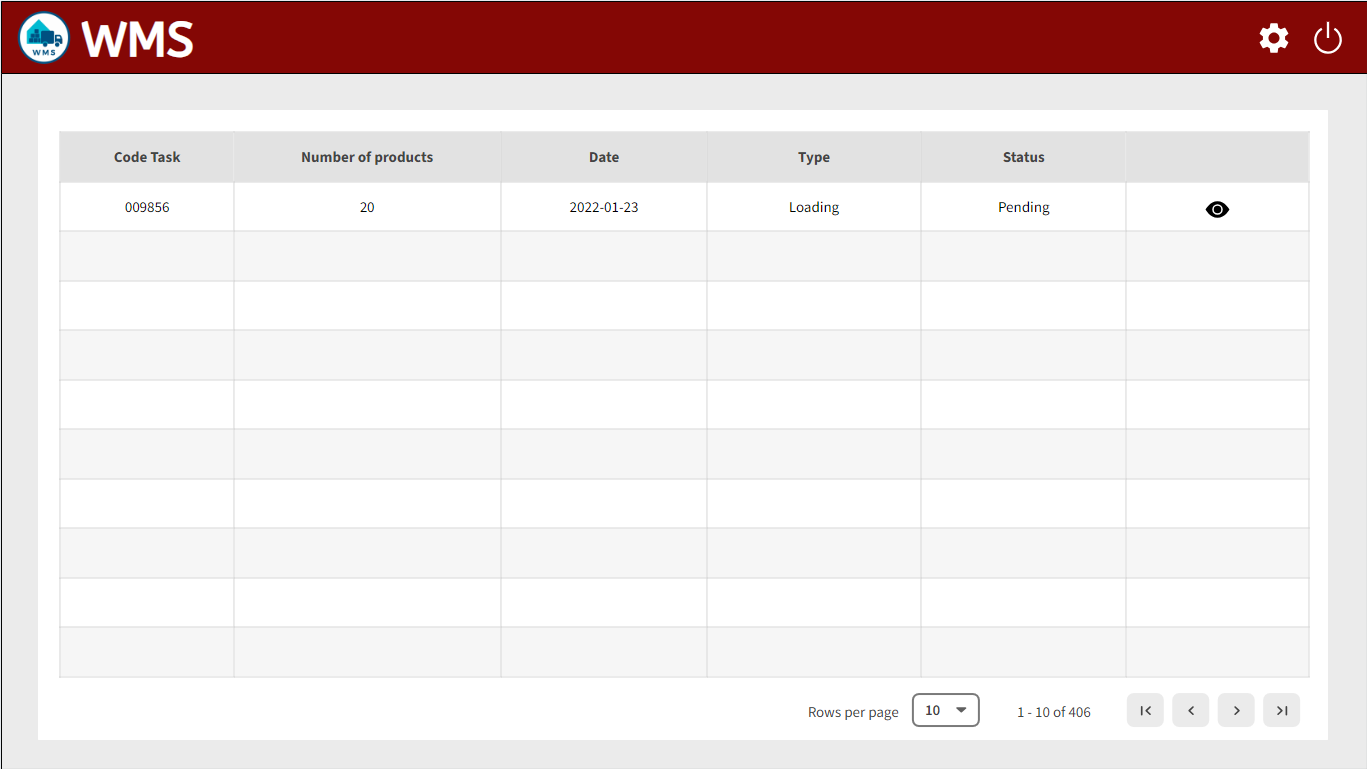
\includegraphics[width=0.8\textwidth]{document/sections/img/Dashboard.png}
    \caption{Home Page Operational}
    \label{fig:homePageOperational}
\end{figure}
Dopo l'autenticazione, l'utente operativo viene reindirizzato alla propria home page.
L'Home Page è strutturata in diverse sezioni chiave:
\begin{itemize}
    \item \textbf{Panoramica delle Attività}: Una tabella centrale che mostra i task attuali dell'utente.
    \item \textbf{Navigazione Intuitiva}: La sidebar a sinistra offre accesso rapido alle principali funzionalità.
    \item \textbf{Azioni Rapide}: Accanto a ciascun task nella tabella, è presente un'icona \textbf{View} che permette di visualizzare i dettagli del task specifico.
\end{itemize}

\begin{figure}[H]
    \centering
    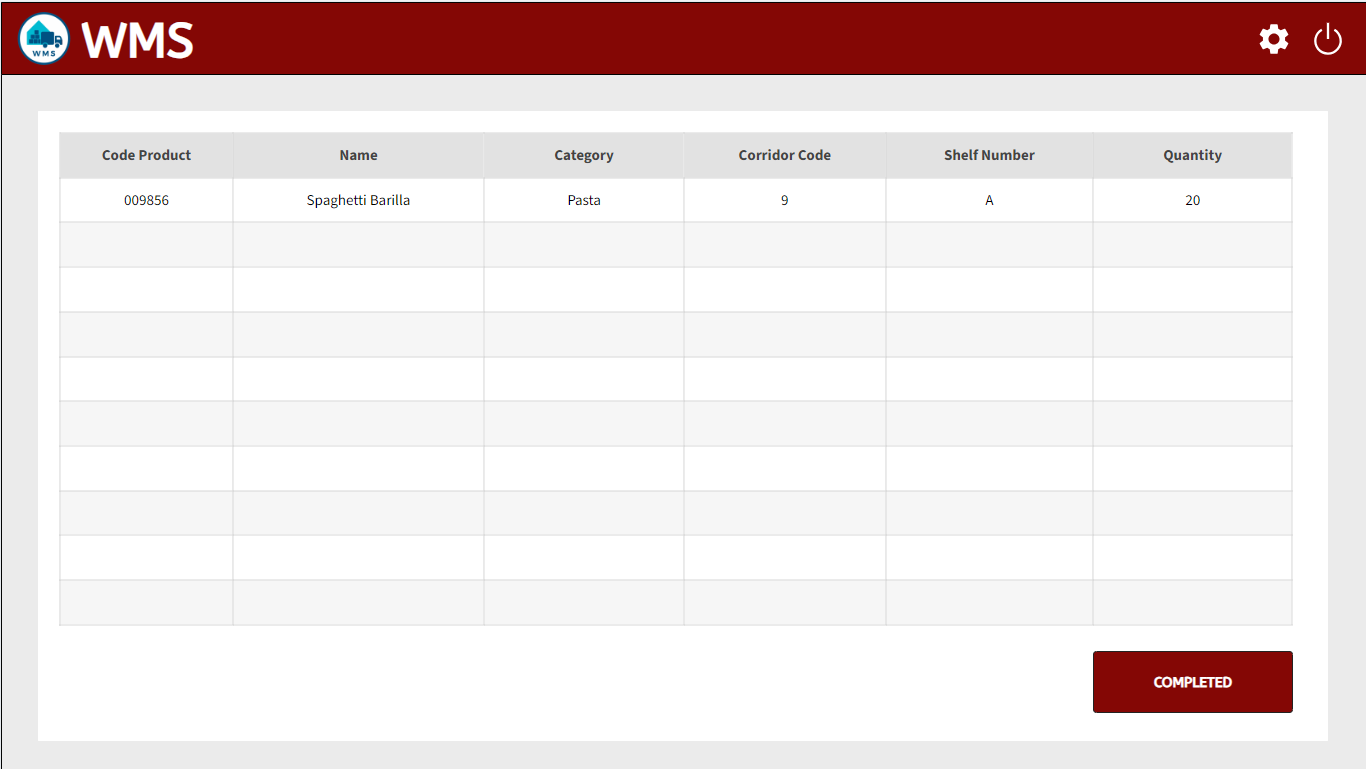
\includegraphics[width=0.8\textwidth]{document/sections/img/taskPageOp.png}
    \caption{Operational's Task View Page}
    \label{fig:taskPageOp}
\end{figure}
Cliccando sull'icona \textbf{View} accanto ad un task, l'utente operativo viene reindirizzato alla pagina di
visualizzazione dei dettagli del task selezionato.\\
Questa pagina fornisce una visualizzazione tabellare, mostrando tutte le informazioni chiave per ogni prodotto
coinvolto nel task.\\
Nella parte inferiore della pagina, è presente un pulsante \textbf{COMPLETED} che consente all'utente di
segnare il task come completato.


\subsection{Design architetturale}
Per quanto riguarda l'architettura del sistema, essa è stata progettata a partire dallo stack MERN che
comprende le seguenti tecnologie:
\begin{itemize}
    \item MongoDB
    \item Express
    \item React
    \item Node.js
\end{itemize}
\subsubsection{Architettura generale}

L'architettura si compone di tre parti principali: il frontend realizzato con React\cite{react}, il backend
realizzato con Node.js e Express, e infine la parte di database per memorizzare i dati dell'applicazione
realizzata con MongoDB.\\ Internamente sono state utilizzate ulteriori tecnologie come Socket.IO
per implementare la comunicazione e l'interoperabilità tra le componenti principali.

\subsubsection{Backend e Database}
Per realizzare il sistema di backend, si è deciso di adottare un’architettura a microservizi. Sono stati individuati sei microservizi principali:

\begin{itemize}
    \item \textbf{Gateway}: si occupa di smistare le comunicazioni ai diversi microservizi.
    \item \textbf{Logistic}: si occupa di gestire le operazioni logistiche e la movimentazione delle risorse all'interno del magazzino.
    \item \textbf{Order}: si occupa del processo di gestione degli ordini, inclusa la creazione, l'elaborazione e l'evasione degli ordini.
    \item \textbf{Product}: si occupa della gestione dell'anagrafica dei prodotti.
    \item \textbf{Task}: si occupa di gestire le attività o i compiti assegnati agli utenti, garantendo il coordinamento e il monitoraggio delle attività in corso.
    \item \textbf{User}: si occupa di gestire l'autenticazione e la registrazione utenti.
\end{itemize}

Si osserva inoltre che:
\begin{itemize}
    \item Ogni microservizio utilizza lo stesso database, suddiviso in sezioni dedicate a ciascun servizio.
    \item Esiste un gateway responsabile di interconnettere l'applicazione con tutti i servizi, garantendo che tutte le comunicazioni, sia in arrivo che in partenza dal client, transitino attraverso di esso.
\end{itemize}

\begin{figure}[H]
    \centering
    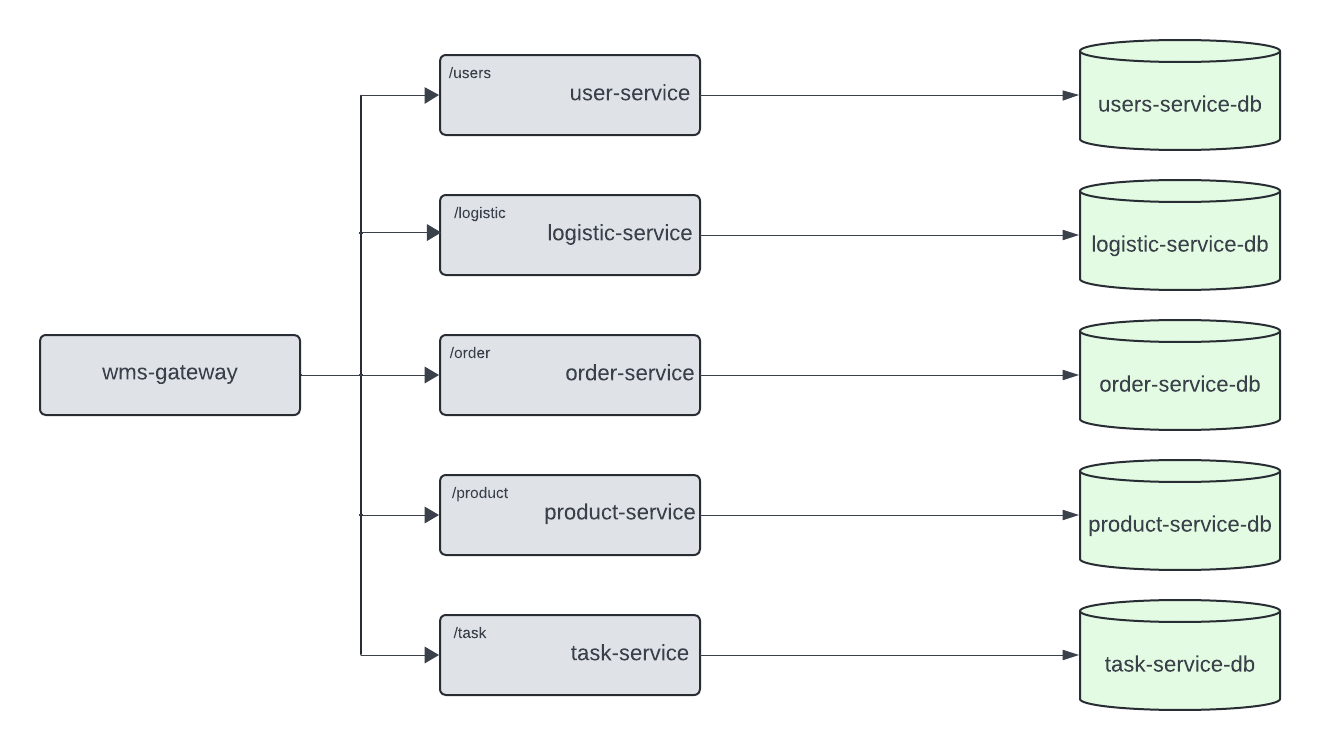
\includegraphics[width=\textwidth]{document/sections/img/architectureServer.png}
    \caption{Architettura del sistema di backend}
    \label{fig:architectureServer}
\end{figure}
Le interazioni nel sistema coinvolgono principalmente il Client e i vari microservizi, con il Gateway
che funge da intermediario.\\Quando il Client invia richieste al backend, il Gateway può indirizzare la
comunicazione verso uno dei microservizi per ottenere informazioni specifiche.\\ Questo approccio assicura
che tutte le interazioni tra il Client e i microservizi avvengano attraverso il Gateway, garantendo una
gestione centralizzata e sicura delle richieste e delle risposte nel sistema.

\begin{figure}[H]
    \centering
    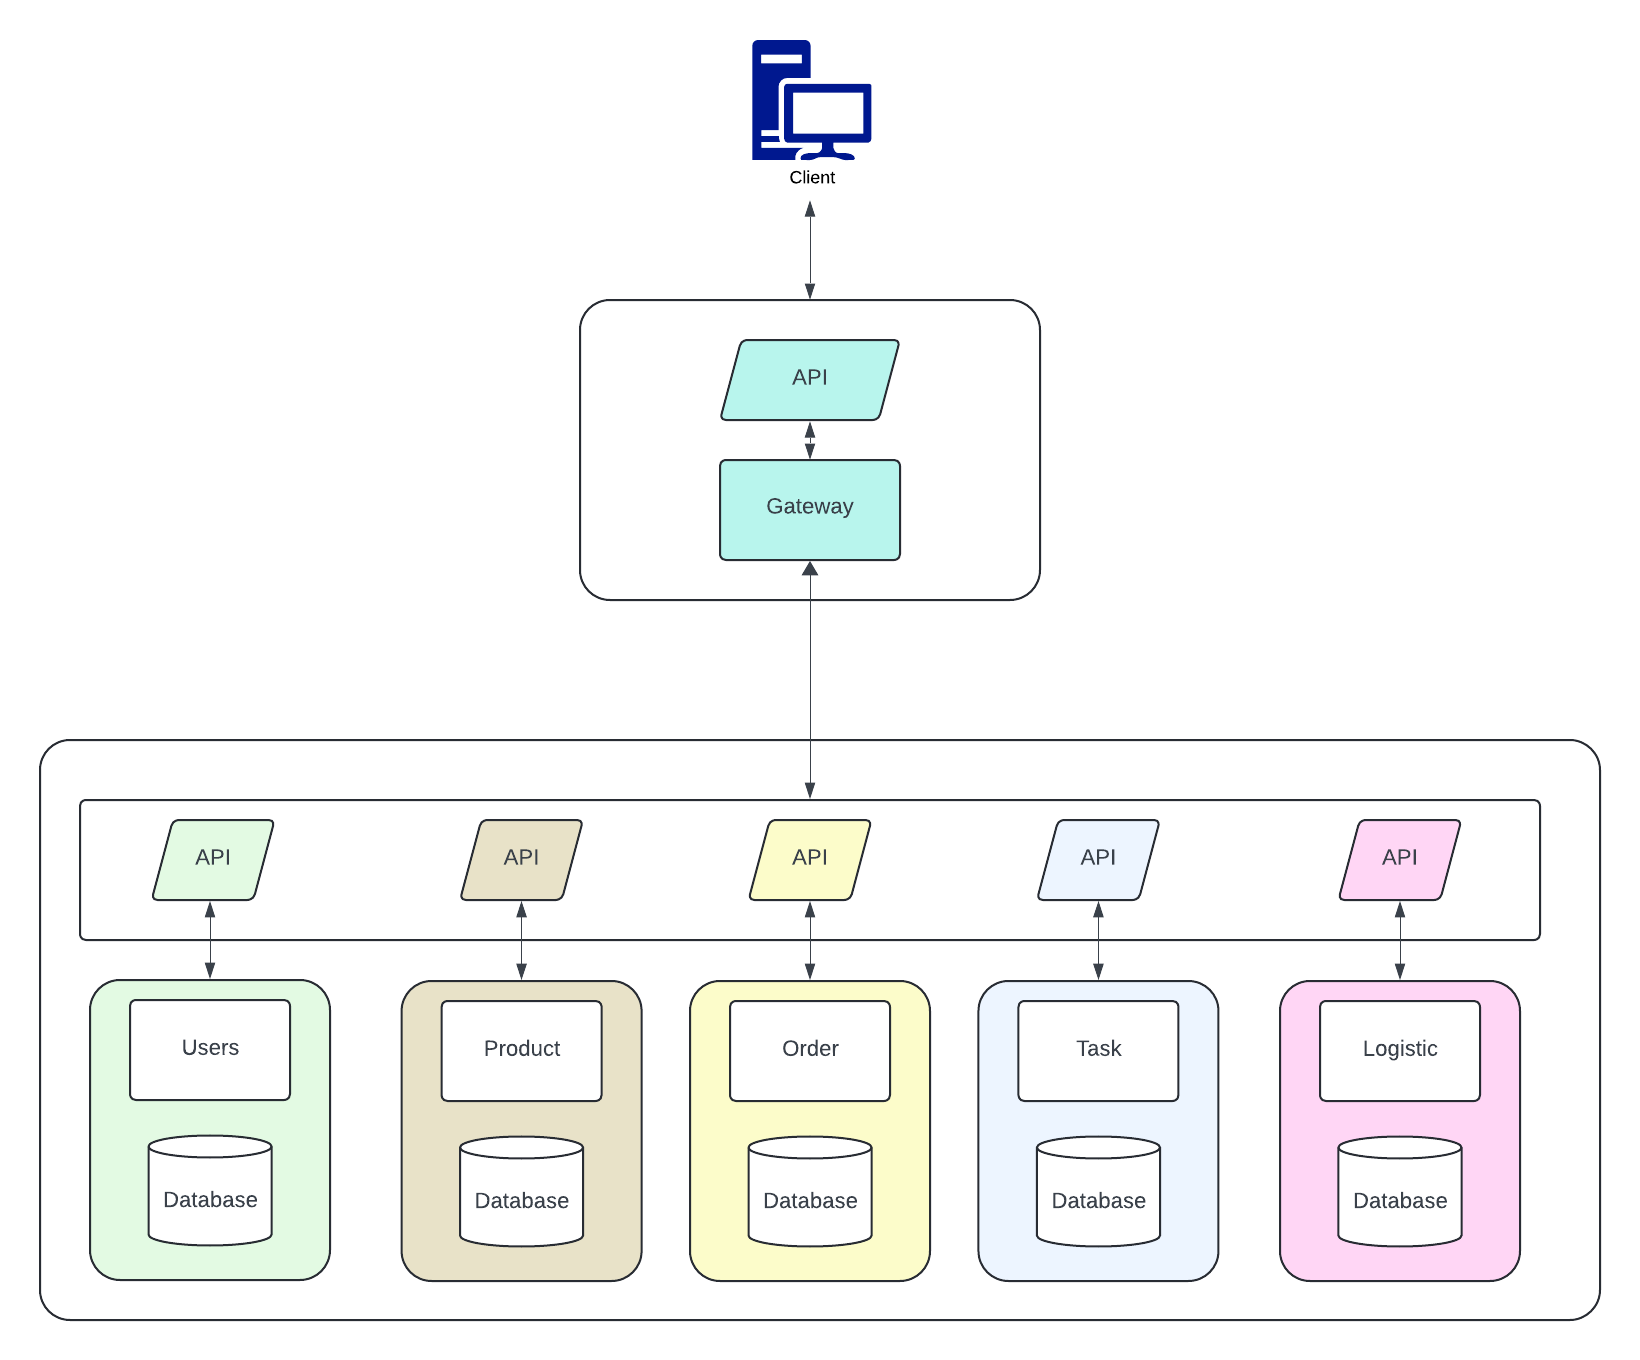
\includegraphics[width=\textwidth]{document/sections/img/serviceInteractions.png}
    \caption{Interazione tra il Client e i Microservizi}
    \label{fig:serviceInteractions}
\end{figure}

Di seguito viene mostrato il comportamento del server nel caso in cui un membro del personale amministrativo
effettui il login.\\ Nell’esempio in questione i servizi coinvolti sono:

\begin{itemize}
    \item \textbf{Product}: si occupa dell'inserimento, aggiornamento, rimozione e visualizzazione dei prodotti all'interno del magazzino.
    \item \textbf{Order}: si occupa dell'inserimento, aggiornamento e monitoraggio degli ordini effettuati.
    \item \textbf{Task}: si occupa dell'assegnazione e monitoraggio dei task attribuiti agli operatori di magazzino.
    \item \textbf{Logistic}: si occupa della gestione della logistica del magazzino, in particolare monitora la posizione dei prodotti all'interno del magazzino.
    \item \textbf{Users}: si occupa di gestire autenticazione e registrazione di ogni utente.
    \item \textbf{Gateway}: si occupa di smistare le comunicazioni ai diversi microservizi.
\end{itemize}

Quando un utente vuole accedere al sistema, inserirà le proprie credenziali tramite il Client, il quale
le invierà al Gateway.\\ Quest'ultimo, a sua volta, inoltrerà le credenziali al microservizio \textbf{Users}.\\
Il microservizio \textbf{Users} restituirà al Gateway le informazioni di avvenuto o negato login, il quale
le inoltrerà al Client. \\In una situazione analoga, quando l'utente desidera accedere a specifiche informazioni,
il Client invia una richiesta al Gateway, il quale la inoltra al relativo microservizio.\\Ad esempio, consideriamo
il flusso per recuperare le informazioni sui task:

Dopo aver effettuato l'accesso, il Client invierà una richiesta al microservizio \textbf{Task} tramite
il Gateway.\\ Questo microservizio si occuperà quindi di restituire tutte le informazioni relative ai task
assegnati al personale operativo.\\ In seguito, verrà inviata un'altra richiesta al
microservizio \textbf{Product} per ottenere ulteriori dettagli sui prodotti inclusi nel task operativo.

\begin{figure}[H]
    \centering
    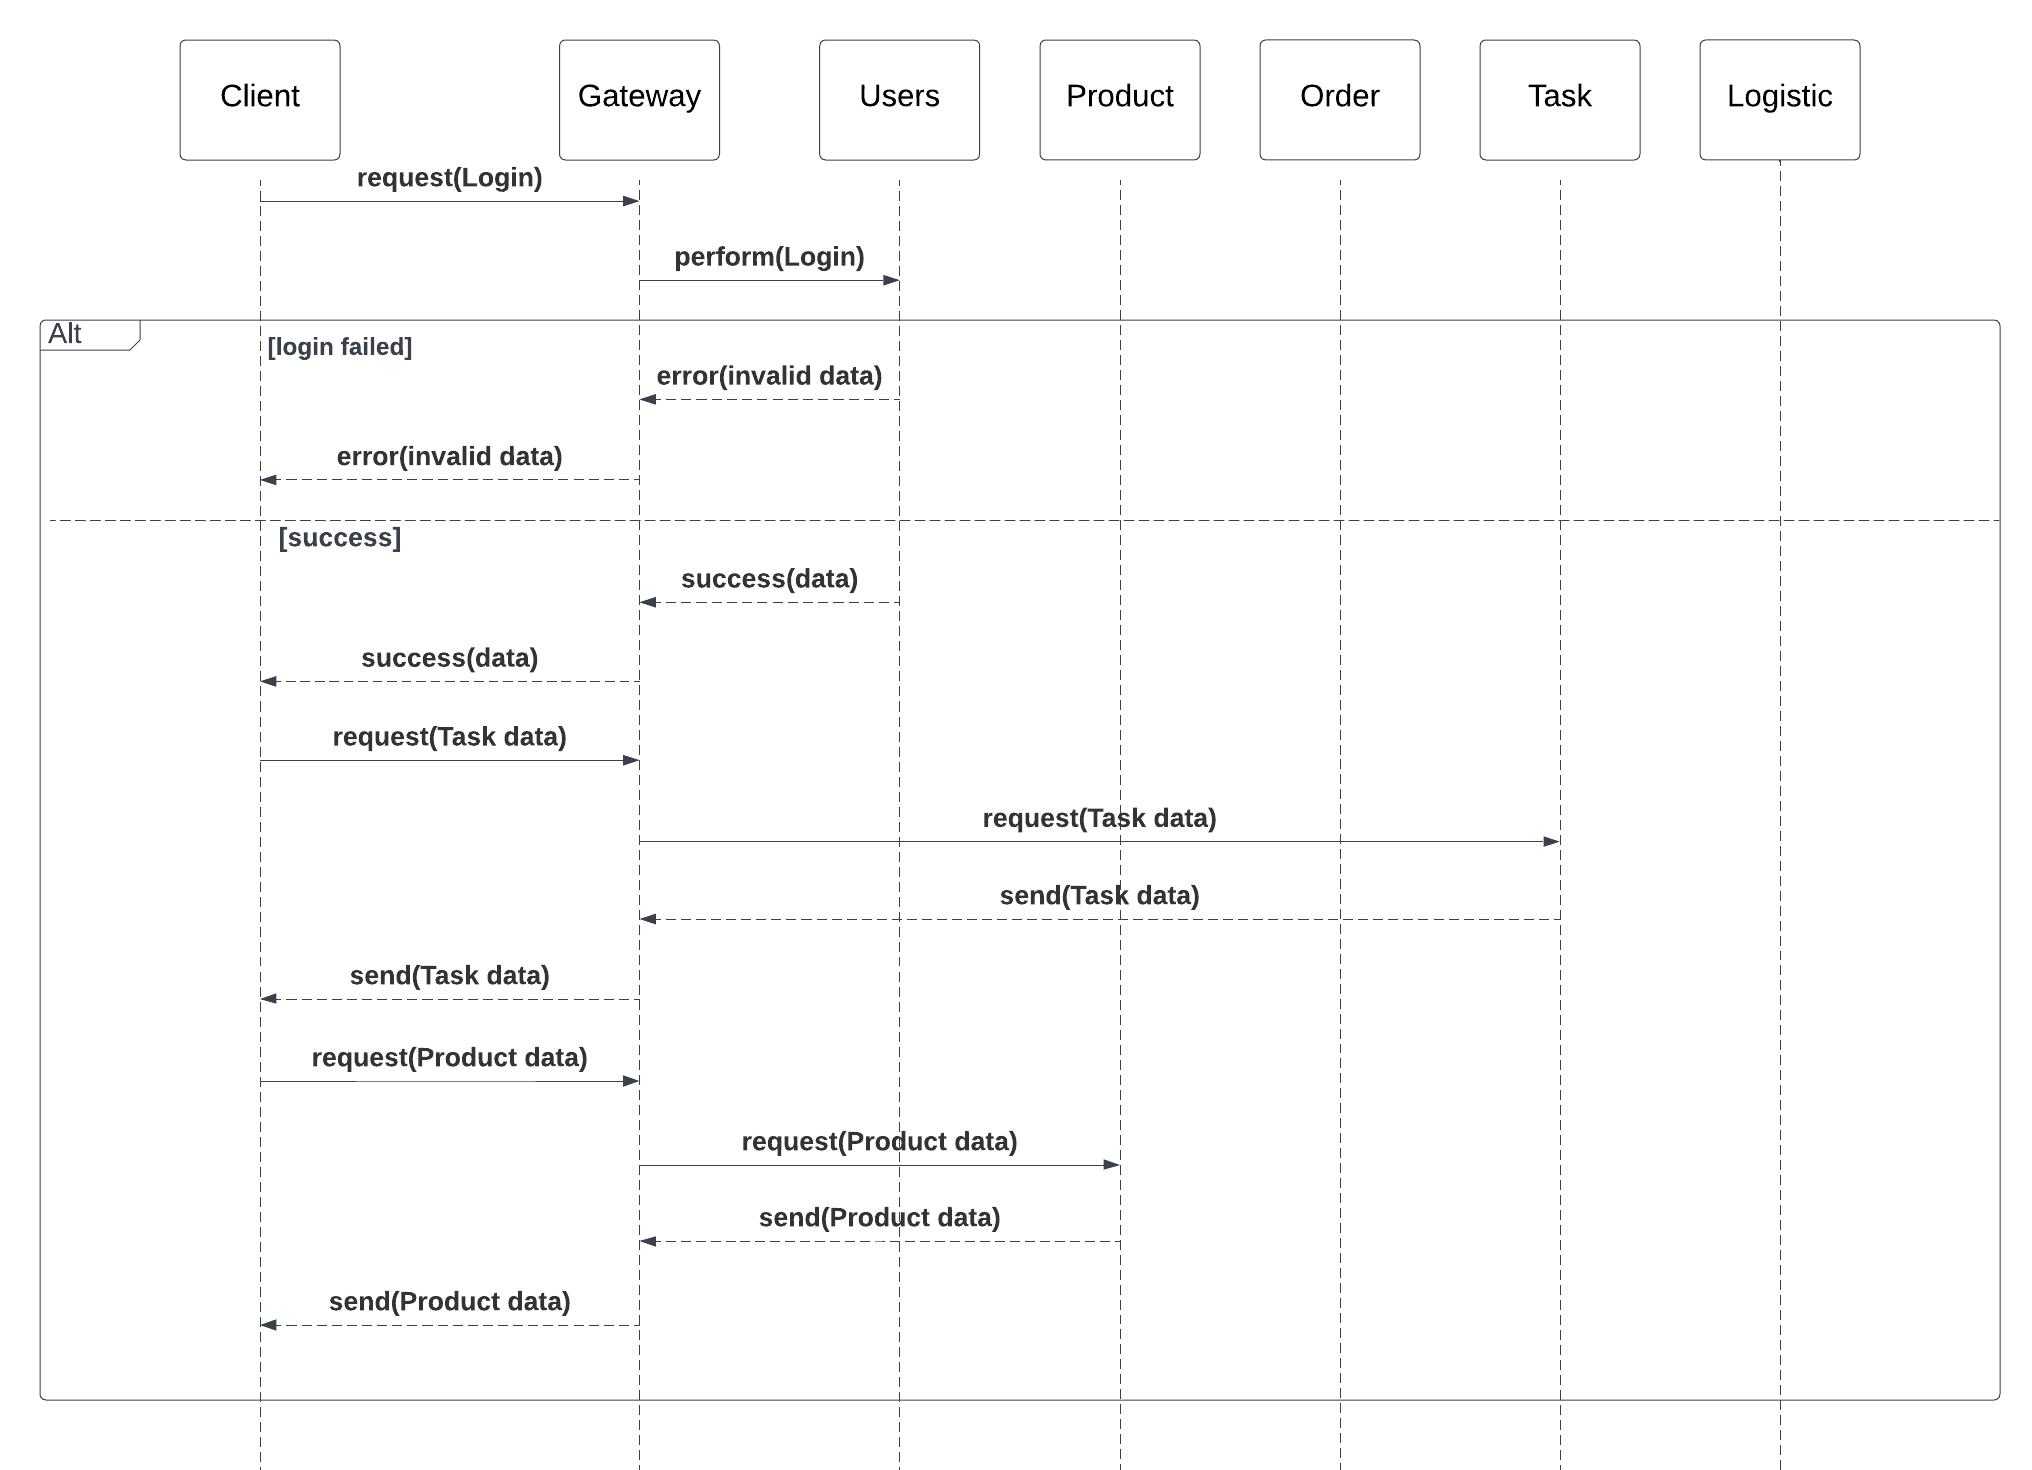
\includegraphics[width=\textwidth]{document/sections/img/sequenceDiagram.png}
    \caption{Diagramma di Sequenza delle Interazioni}
    \label{fig:sequenceDiagram}
\end{figure}
Il design architetturale del backend `e stato dunque organizzato adottando il \textbf{Domain-Driven Design (DDD)}.
Questa è una metodologia di progettazione del software che si concentra sulla comprensione e sulla modellazione
del dominio di business all'interno del quale opera un'applicazione.\\ Nell'ambito dei microservizi,
l'adozione del DDD è particolarmente vantaggiosa in quanto consente di suddividere il complesso dominio
aziendale in sottodomini più gestibili, ciascuno dei quali rappresenta un microservizio.\\ Questo aiuta a
mantenere la chiarezza e la coerenza all'interno di ciascun servizio, facilitando la comprensione e la
manutenzione del codice.\\
I building blocks del DDD forniscono una struttura organizzativa per ciascun microservizio,
definendo ruoli e responsabilità chiare per ciascun componente.\\ Ecco una breve panoramica di come i building
blocks vengono utilizzati nei microservizi:

\begin{itemize}
    \item \textbf{Entità (Entities)}: rappresentano gli oggetti principali del dominio.
    \item \textbf{Factory}: sono responsabili della creazione di nuove istanze di oggetti complessi all'interno del dominio.
    \item \textbf{Repository}: fungono da interfacce tra database e il microservizio per l'accesso ai dati. Gestiscono le operazioni di persistenza dei dati e forniscono metodi per recuperare e manipolare gli oggetti del dominio.
    \item \textbf{Service}: contengono la logica di business e coordinano le operazioni cruciali all'interno di un dominio specifico. Si occupano di gestire operazioni complesse che coinvolgono una o più entità, definite all'interno del microservizio stesso.
\end{itemize}

\subsubsection{Frontend}
La parte di frontend è stata progettata seguendo il pattern \textit{MVC} (Model-View-Controller) per favorire la manutenibilità ed estendibilità del codice. Di seguito sono dettagliati i componenti principali di questo pattern nell'ambito dell'applicazione:

\begin{itemize}
    \item \textbf{Model}: I modelli gestiscono la struttura dei dati. Questi modelli sono responsabili della gestione dei dati senza occuparsi della presentazione o dell'interazione con l'utente.
    
    \item \textbf{View}: I Componenti React agiscono come la View nel pattern MVC, gestendo la presentazione e l'interazione con l'utente. Queste componenti utilizzano gli hook di React, come \textit{useState} per la gestione dello stato interno e \textit{useEffect} per la gestione degli effetti collaterali, per reagire ai cambiamenti e presentare i dati all'utente in modo reattivo.
    
    \item \textbf{Controller}: I Controller mediando l'interazione tra la View e il Model. Gestiscono la logica di business, come il recupero, l'aggiunta, la modifica e l'eliminazione degli ordini, e comunicano con il backend attraverso degli specifici service creati per gestirne le relative chiamate asincrone.
\end{itemize}

Per ogni \textit{Component}, che nell'applicativo rappresentano la vista del pattern MVC, è stato creato un \textit{Controller} che si occupa di mediare tra la vista e il relativo \textit{Model}, garantendo una chiara separazione delle responsabilità e facilitando lo sviluppo e la manutenzione del codice.

\subsection{Storyboard}

L'applicazione finale si è evoluta significativamente rispetto ai mockup iniziali realizzati in fase di progettazione.\\
Le modifiche apportate sono state guidate dai feedback e dalle interazioni avute con gli utenti.\\
Questo processo iterativo ha permesso di affinare e migliorare l'applicazione, garantendo che le esigenze e le
aspettative degli utenti fossero soddisfatte in maniera ottimale.

\begin{figure}[H]
    \centering
    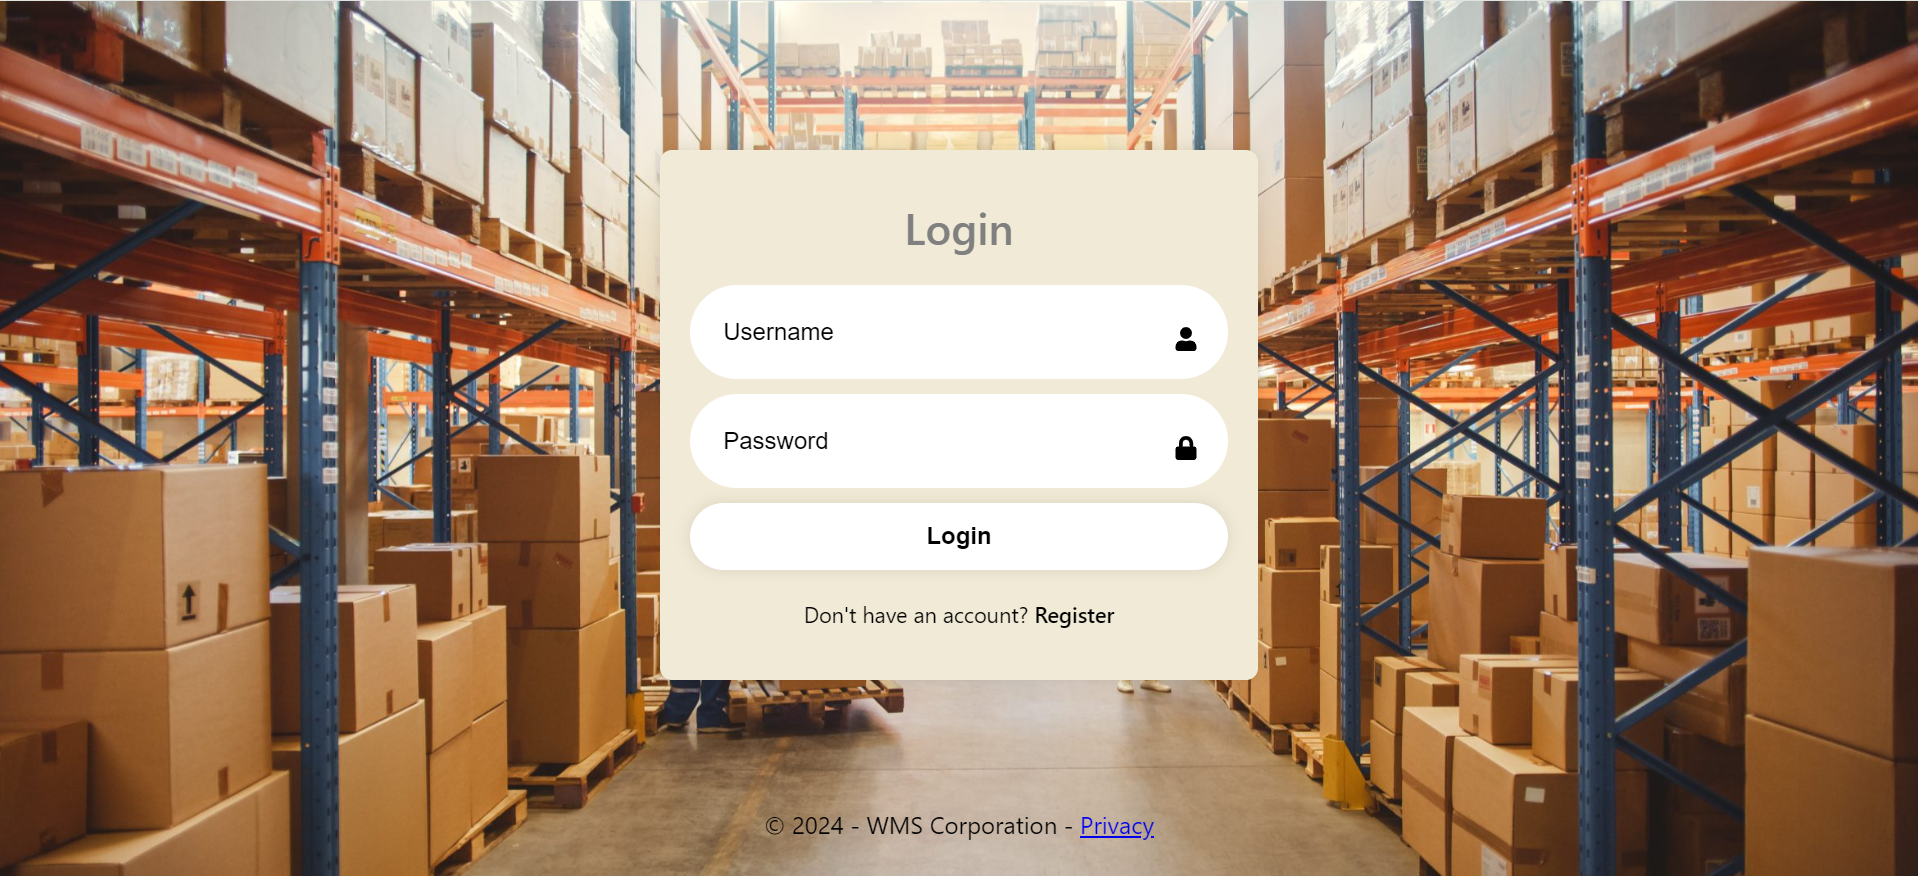
\includegraphics[width=\textwidth]{document/sections/img/Storyboard/login.png}
    \caption{Login Page}
    \label{fig:loginPage}
\end{figure}

La pagina iniziale dell’applicazione si presenta con questa schermata, che consente all’utente, sia esso operativo che
amministrativo, di accedere al sistema inserendo le proprie credenziali.\\
Nel caso in cui l’utente inserisca credenziali non valide, verrà mostrato un messaggio di errore.

\begin{figure}[H]
    \centering
    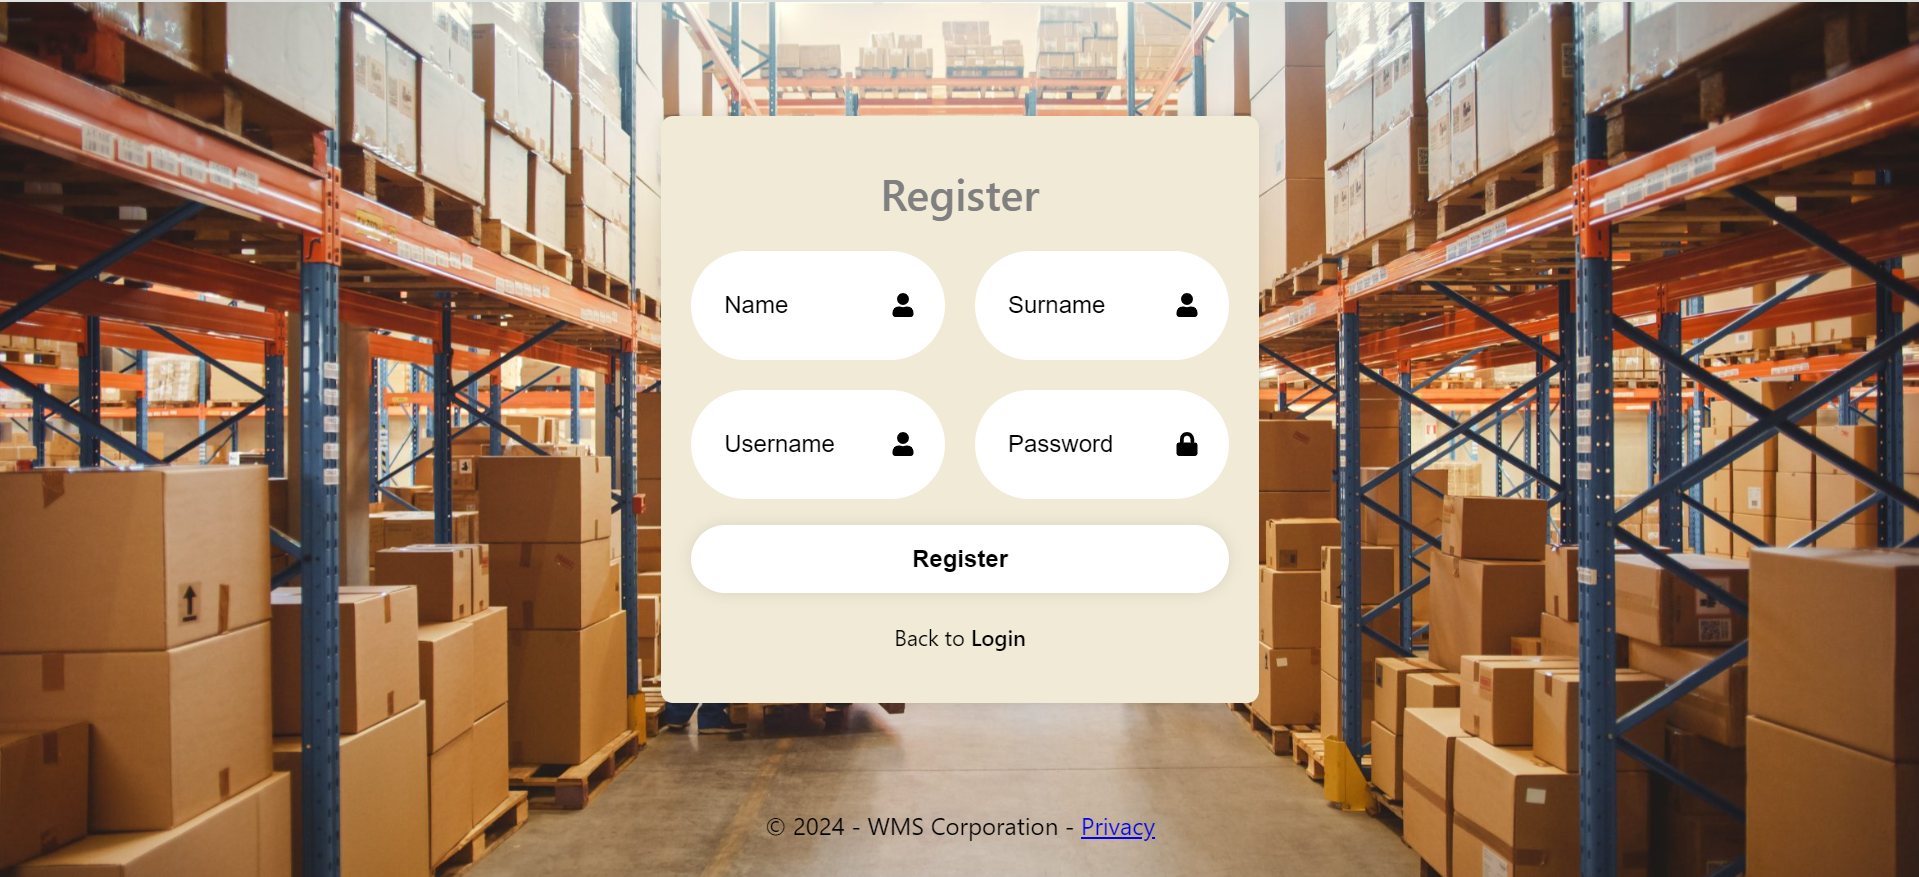
\includegraphics[width=\textwidth]{document/sections/img/Storyboard/register.png}
    \caption{Register Page}
    \label{fig:registerPage}
\end{figure}

Cliccando sul link \textbf{Register} nella pagina di login viene mostra un form per effettuare la registrazione al sistema.
Una volta completata la registrazione si viene reindirizzati alla propria Home Page.

\subsubsection{Admin}

\begin{figure}[H]
    \centering
    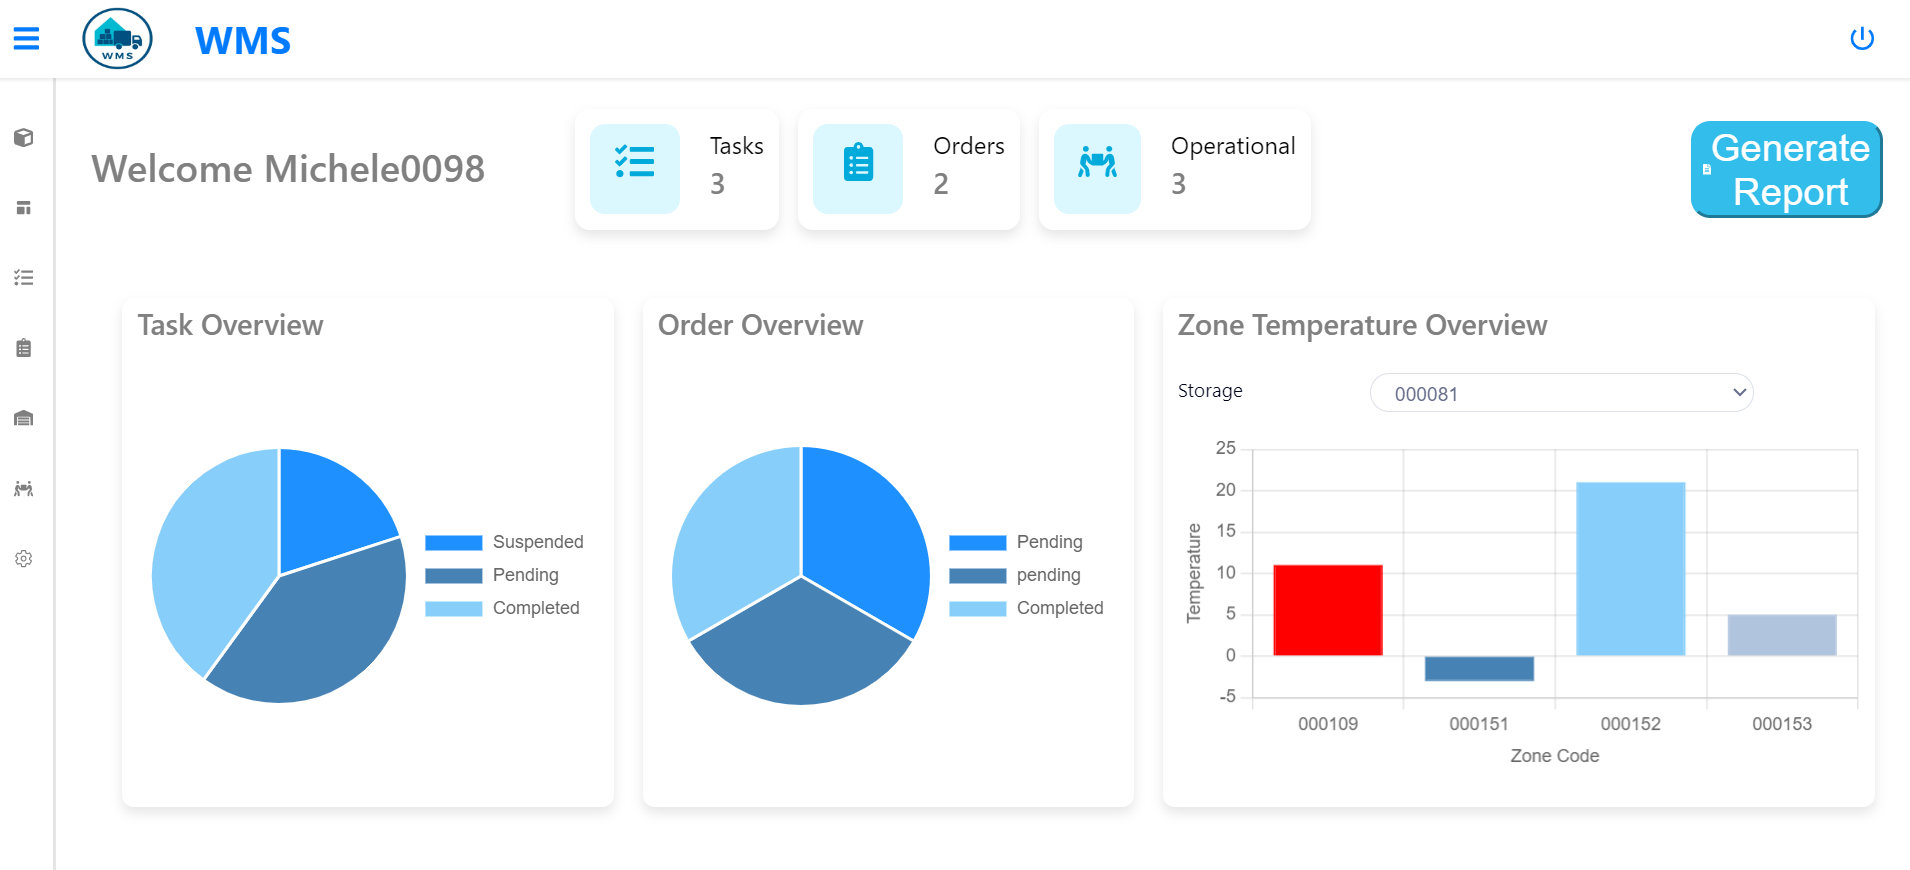
\includegraphics[width=\textwidth]{document/sections/img/Storyboard/homePageAdmin.png}
    \caption{Home Page Admin}
    \label{fig:homePageAdmins}
\end{figure}

L'Home Page dell' Admin offre una panoramica delle principali attività e metriche del magazzino.
In alto, vengono mostrate tre statistiche chiave: il numero di task e ordini non completati, e il numero di utenti
Operational registrati.\\

La sezione centrale include tre grafici:
\begin{itemize}
    \item \textbf{Task Overview}: un grafico a torta che mostra lo stato dei task.
    \item \textbf{Order Overview}: un grafico a torta che rappresenta lo stato degli ordini.
    \item \textbf{Zone Temperature Overview}: un grafico a barre che visualizza le temperature nelle diverse zone del magazzino.
\end{itemize}

Sulla destra è presente un pulsante \textbf{Generate Report} per generare report dettagliati.\\
La sidebar, situata a sinistra, consente una navigazione rapida e intuitiva tra le varie sezioni dell'applicazione.\\
L'header in alto contiene il logo dell'applicazione a sinistra, mentre a destra è presente l'icona per il logout.

\begin{figure}[H]
    \centering
    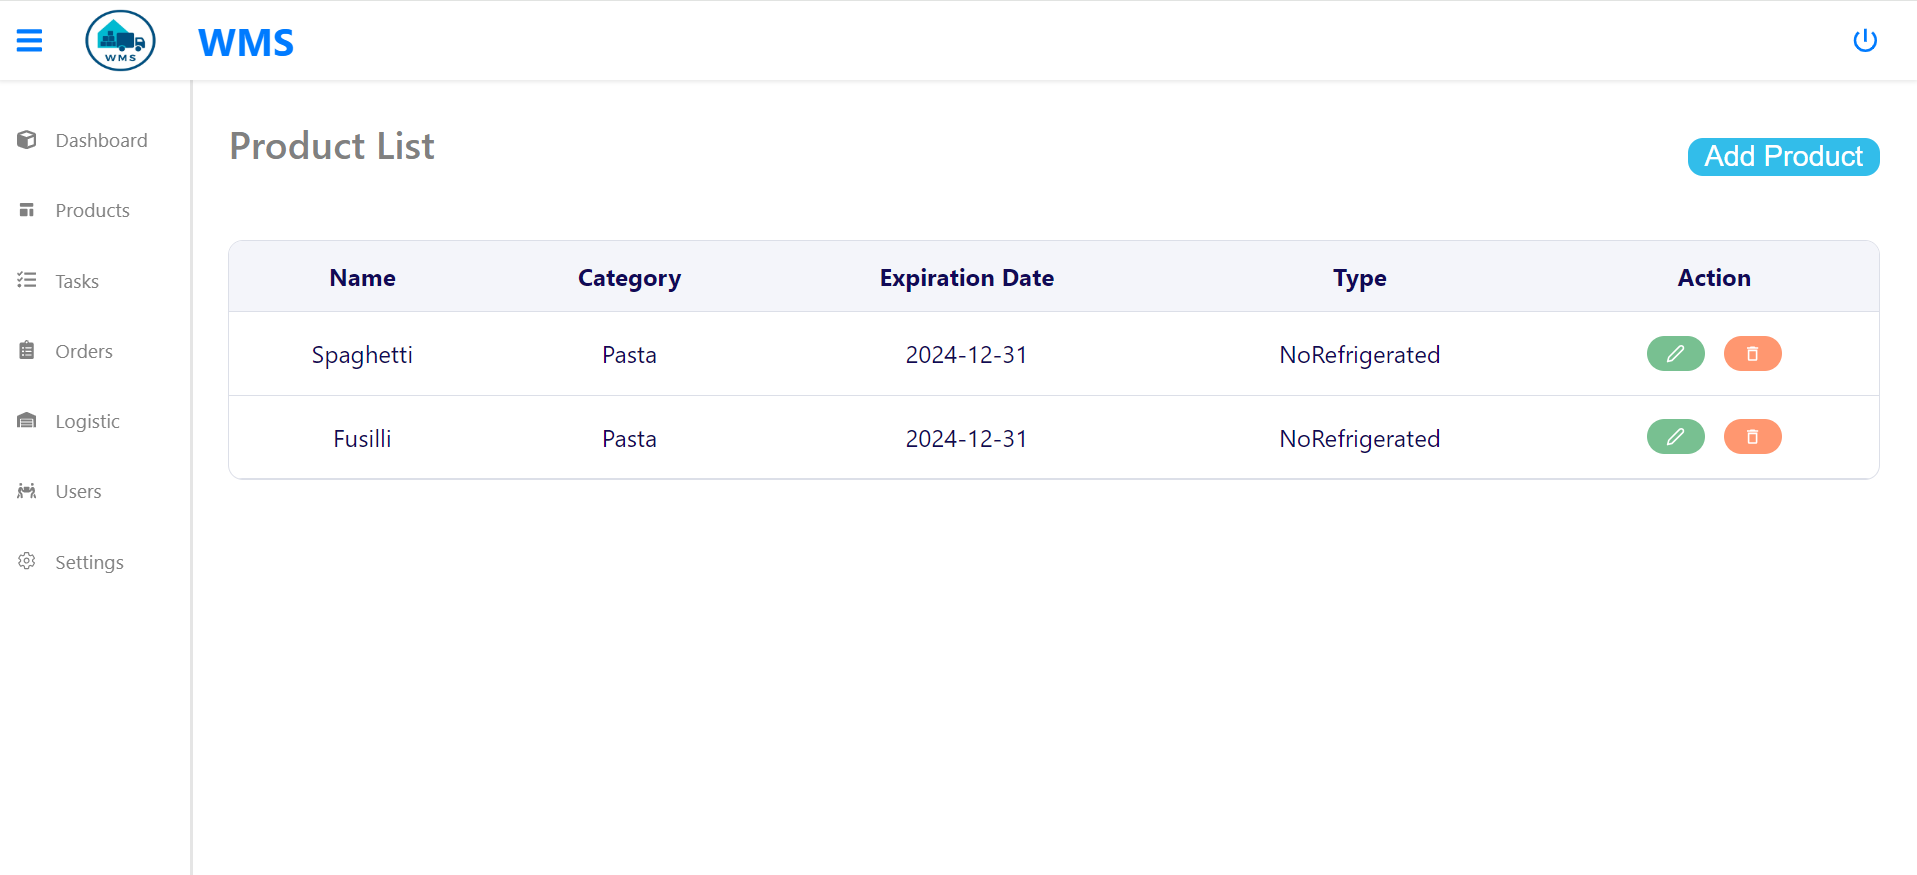
\includegraphics[width=\textwidth]{document/sections/img/Storyboard/productPage.png}
    \caption{Product Page}
    \label{fig:productPages}
\end{figure}

Cliccando sulla voce \textbf{Products} nella sidebar, l'utente viene reindirizzato alla pagina di gestione dei prodotti.\\
Questa pagina offre una visualizzazione tabellare dei prodotti presenti nel magazzino,
mostrando le informazioni chiave per ogni prodotto.\\
Nella colonna di sinistra, sono presenti delle icone che consento di modificare o eliminare il prodotto.\\
In alto a destra è presente un pulsante \textbf{Add Product} che consente di aggiungere nuovi prodotti al sistema.

\begin{figure}[H]
    \centering
    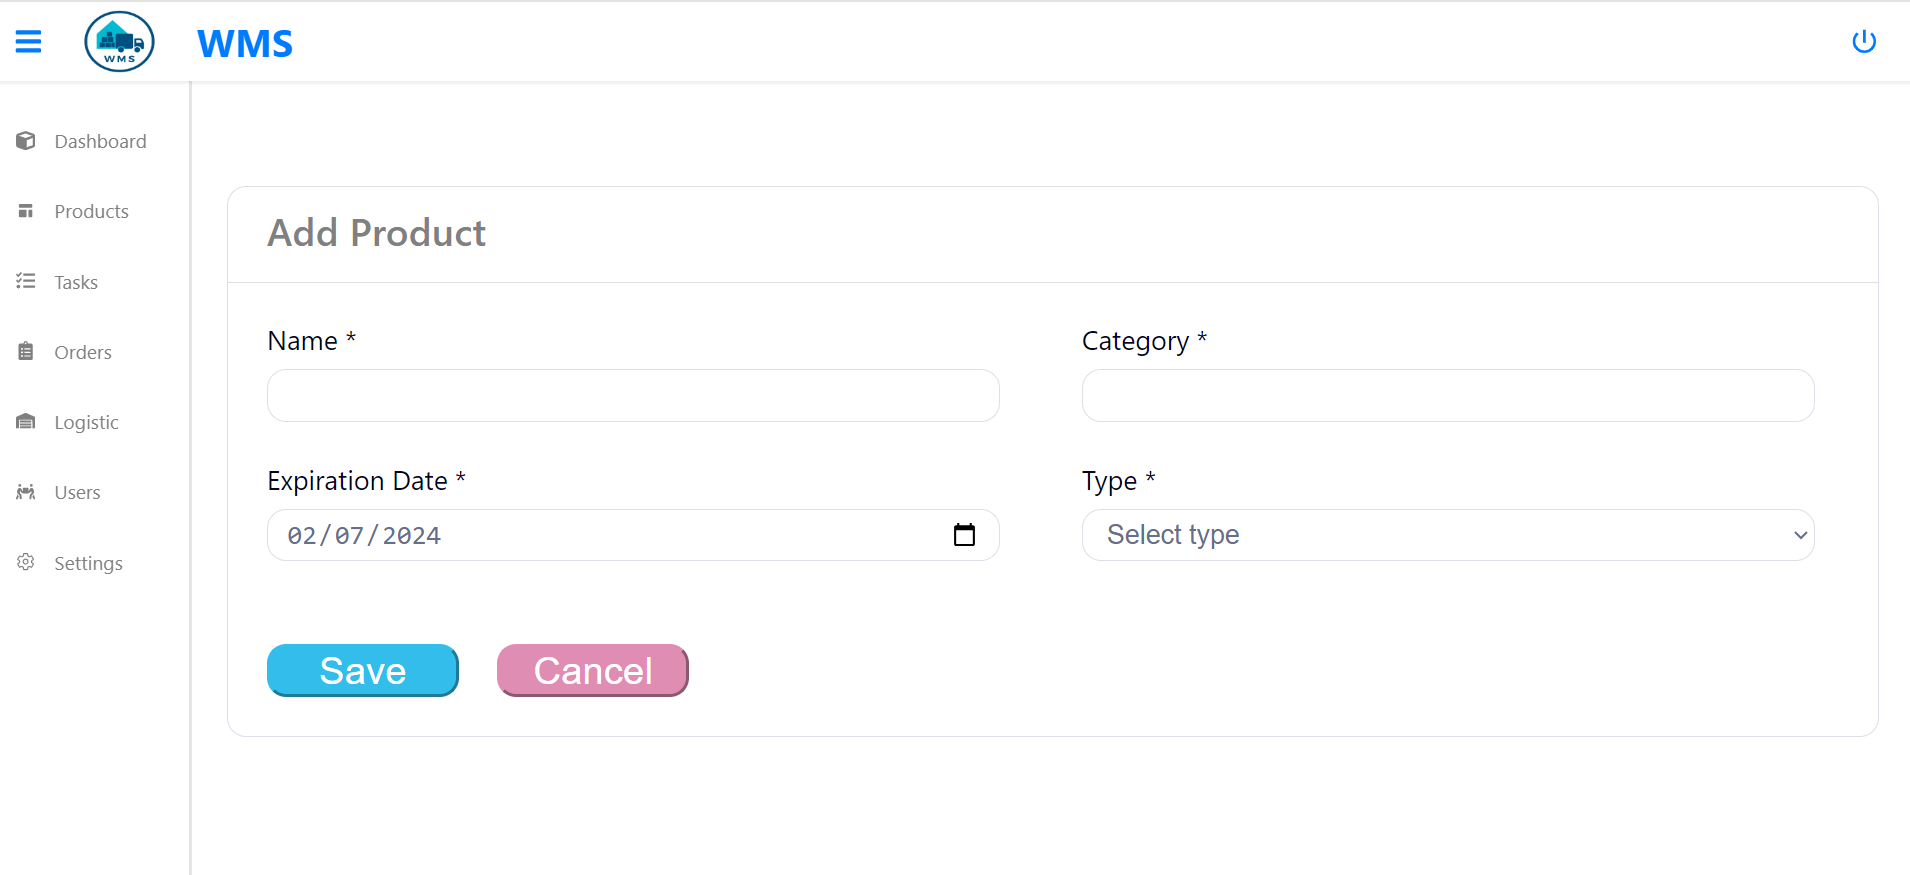
\includegraphics[width=\textwidth]{document/sections/img/Storyboard/addProductPage.png}
    \caption{Add Product Page}
    \label{fig:addProductPages}
\end{figure}

Cliccando sul pulsante \textbf{Add new} nella product page si apre un form, che consente
all'Admin di poter creare un nuovo prodotto.\\
Cliccando sul bottone \textbf{Save} vengono salvati i dati del prodotto, mentre cliccando sul bottone \textbf{Cancel} si torna alla product page.\\
Qualora non venissero inseriti correttamente tutti i dati verrà mostrato un messaggio di errore.

\begin{figure}[H]
    \centering
    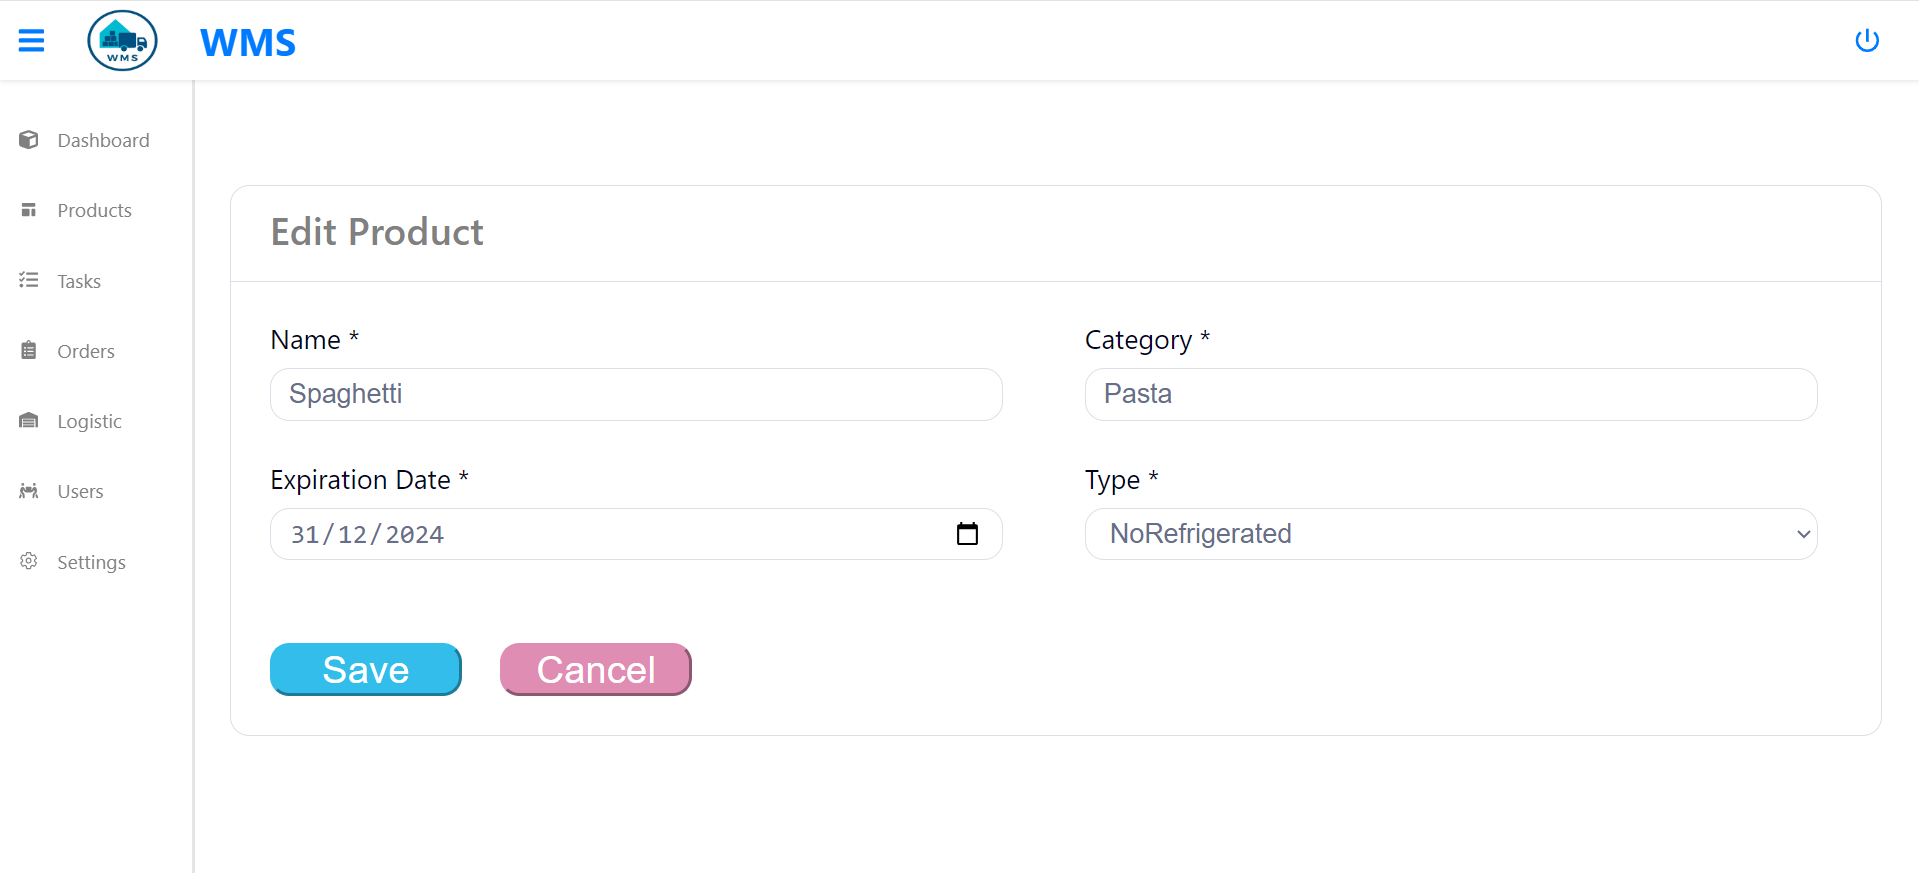
\includegraphics[width=\textwidth]{document/sections/img/Storyboard/editProductPage.png}
    \caption{Edit Product Page}
    \label{fig:editProductPage}
\end{figure}

Cliccando sull'icona \textbf{edit} di un determinato prodotto, nella product page, si apre un form che consente
all'Admin di poter modificare i dettagli del prodotto.\\
Cliccando sul bottone \textbf{Save} vengono salvate le modifiche, mentre cliccando sul bottone \textbf{Cancel} si viene
riportare alla product page.

\begin{figure}[H]
    \centering
    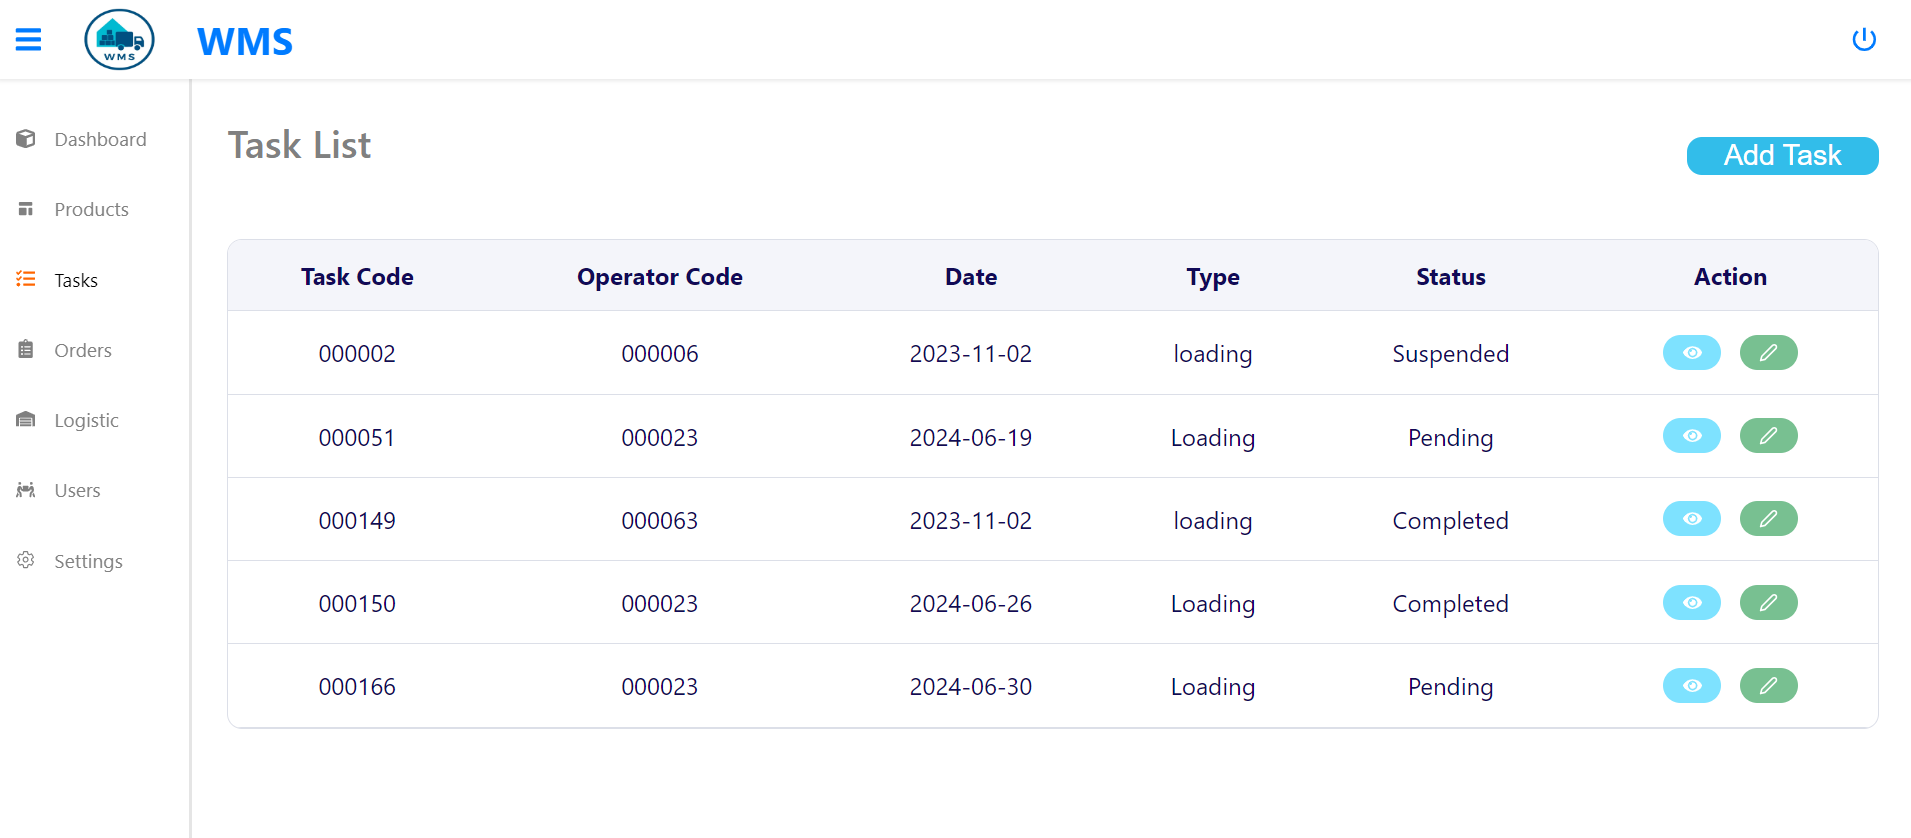
\includegraphics[width=\textwidth]{document/sections/img/Storyboard/taskPage.png}
    \caption{Tasks Page}
    \label{fig:tasksPage}
\end{figure}

Cliccando sulla voce \textbf{Tasks} nella sidebar, l'utente viene reindirizzato alla pagina di gestione dei tasks.\\
Questa pagina offre una visualizzazione tabellare dei task assegnati ai vari operatori,
mostrando le informazioni chiave per ognuno.\\
Nella colonna di destra, sono presenti delle icone che consento di modificare, eliminare oppure visualizzare meglio
i dati di un singolo task.\\
In alto a destra è presente un pulsante \textbf{Add Task} che consente di aggiungere un nuovo task al sistema.

\begin{figure}[H]
    \centering
    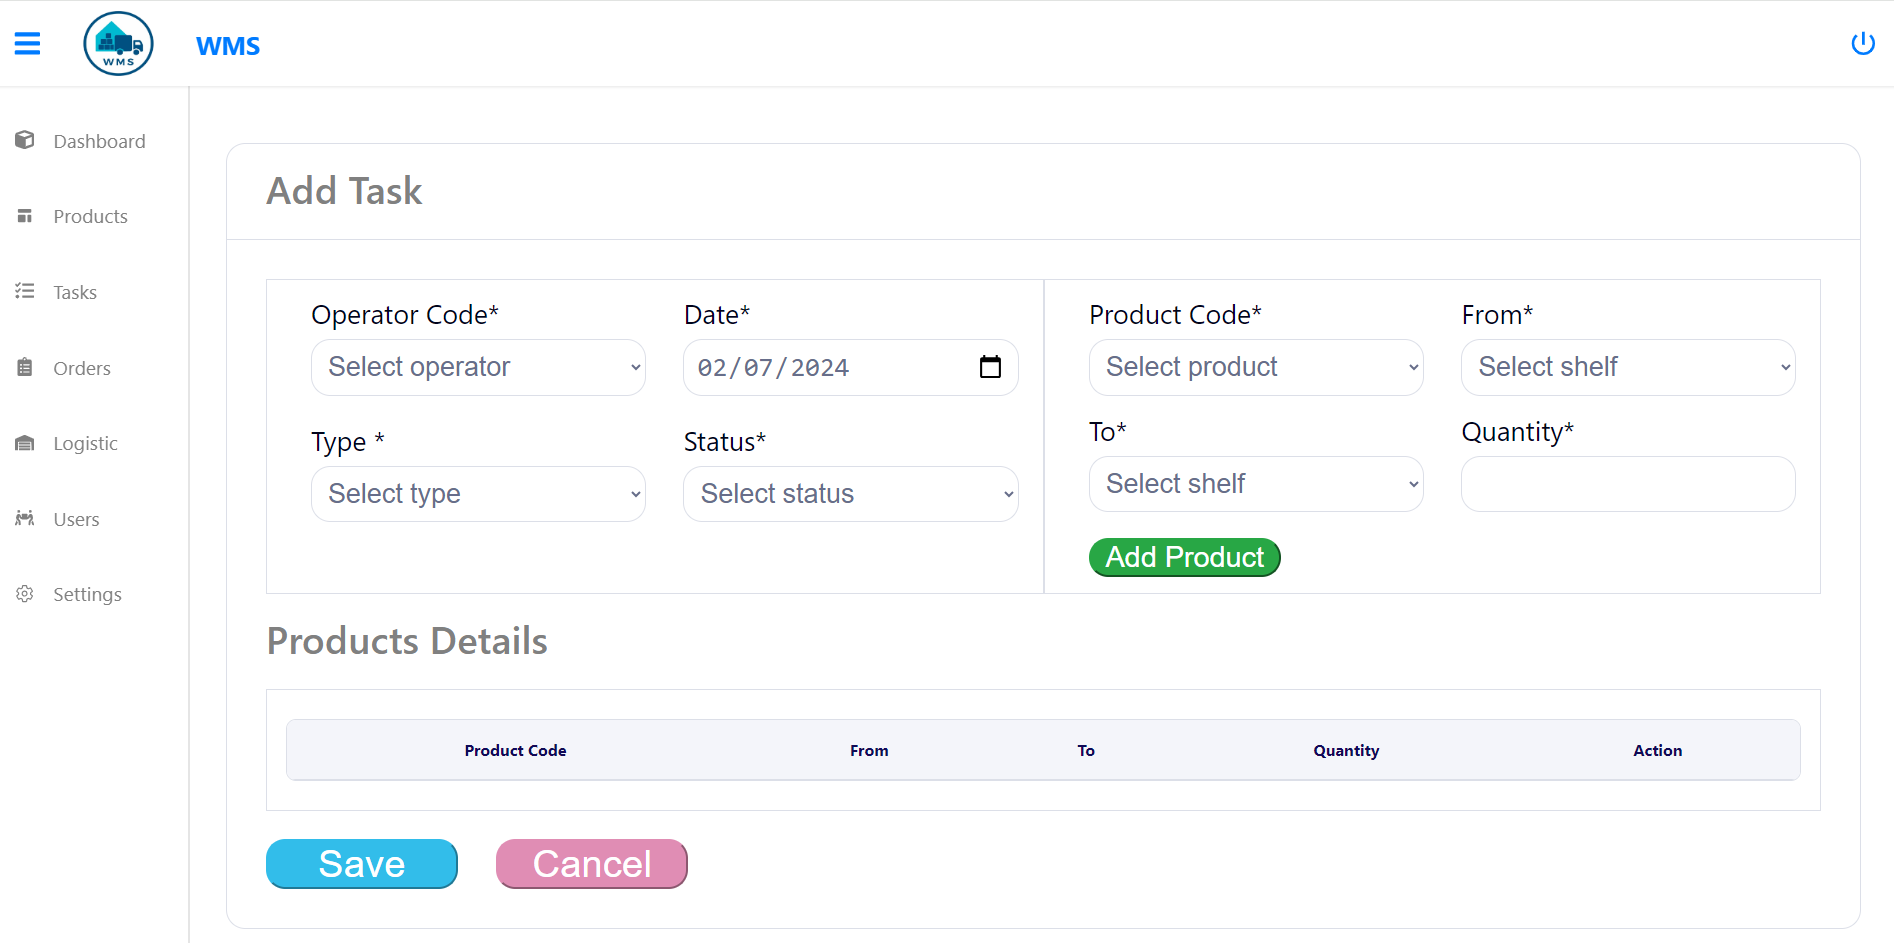
\includegraphics[width=\textwidth]{document/sections/img/Storyboard/addTaskPage.png}
    \caption{Add Task Page}
    \label{fig:addTaskPages}
\end{figure}

Cliccando sul pulsante \textbf{Add new} nella task page si apre un form, che consente
all'Admin di poter creare un nuovo task.\\
Sotto il form, è presente una sezione denominata \textbf{Products Details} che mostra i dettagli dei prodotti inclusi
nel task in formato tabellare.\\Gli utenti possono aggiungere più prodotti al task utilizzando il pulsante \textbf{Add Product}.\\
Infine, in basso, sono presenti i pulsanti \textbf{Save} per salvare il task e \textbf{Cancel} per annullare l'operazione
e tornare alla task page.\\
Qualora non venissero inseriti correttamente tutti i dati verrà mostrato un messaggio di errore.

\begin{figure}[H]
    \centering
    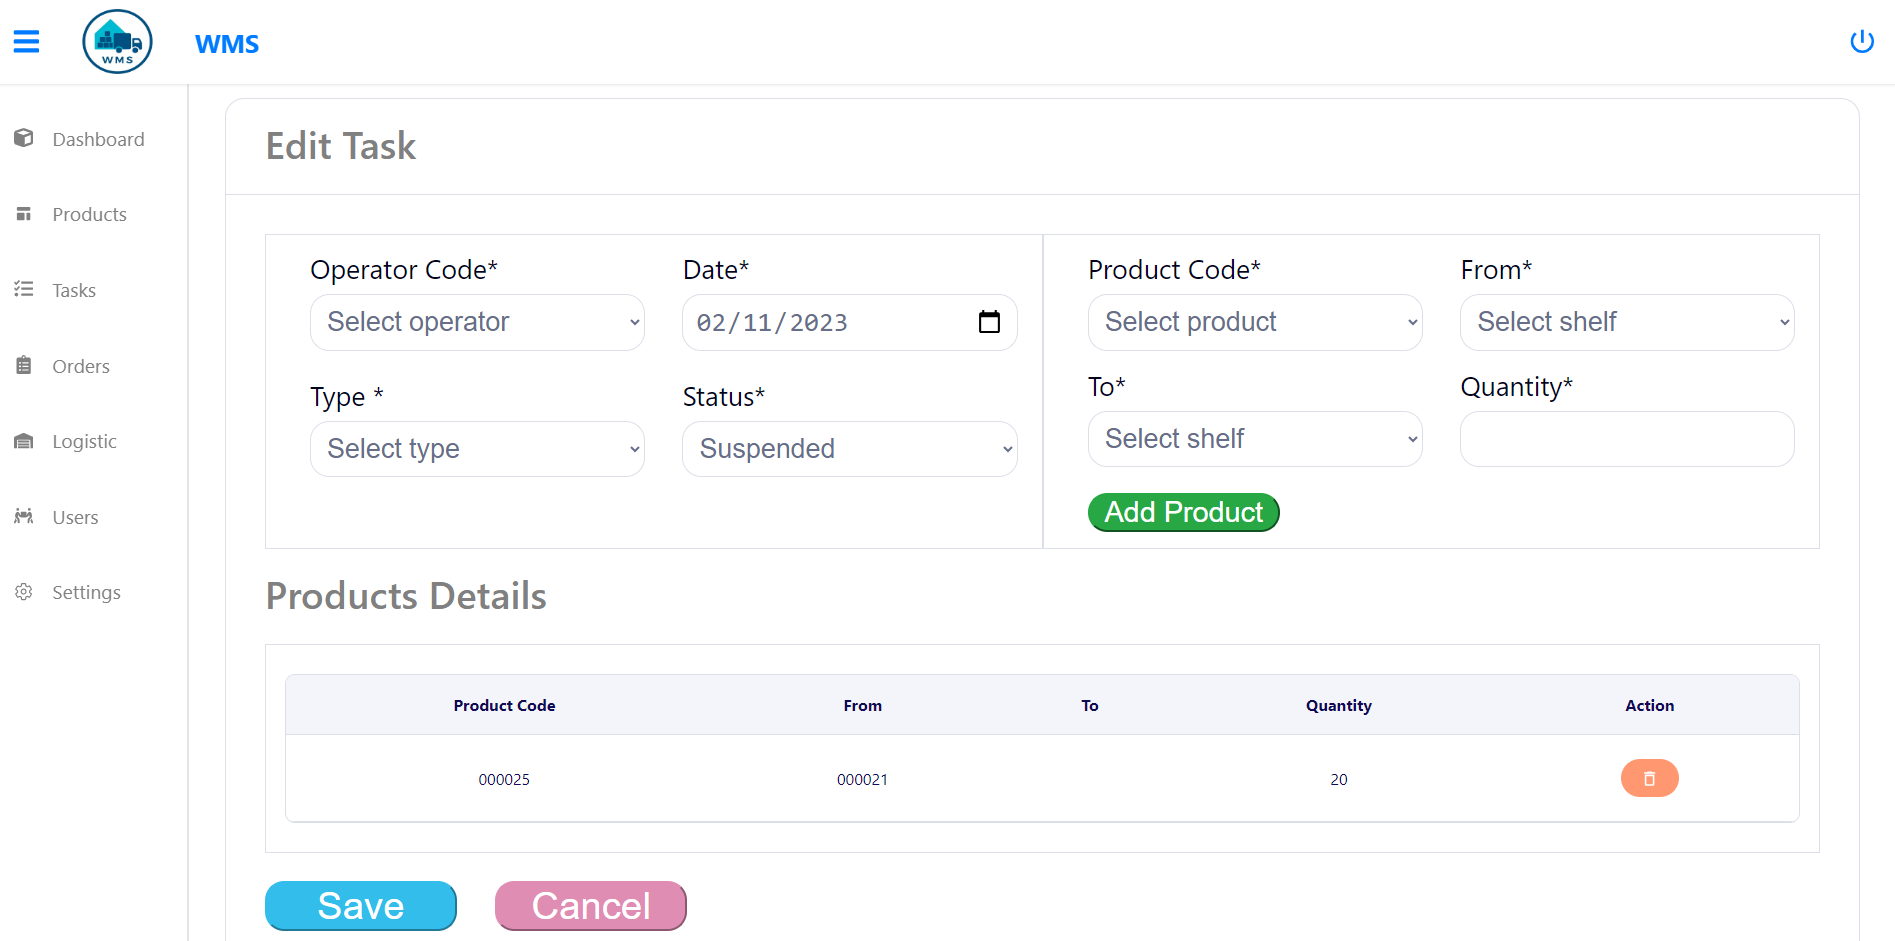
\includegraphics[width=\textwidth]{document/sections/img/Storyboard/editTaskPage.png}
    \caption{Edit Task Page}
    \label{fig:editTaskPage}
\end{figure}

Cliccando sull'icona \textbf{edit} di un determinato task, nella task page, si apre un form simile a quello che
consente di aggiungere un nuovo task, che permette all'Admin di modificarne i dati.\\
Cliccando sul bottone \textbf{Save} vengono salvate le modifiche, mentre cliccando sul bottone \textbf{Cancel} si torna alla task page.

\begin{figure}[H]
    \centering
    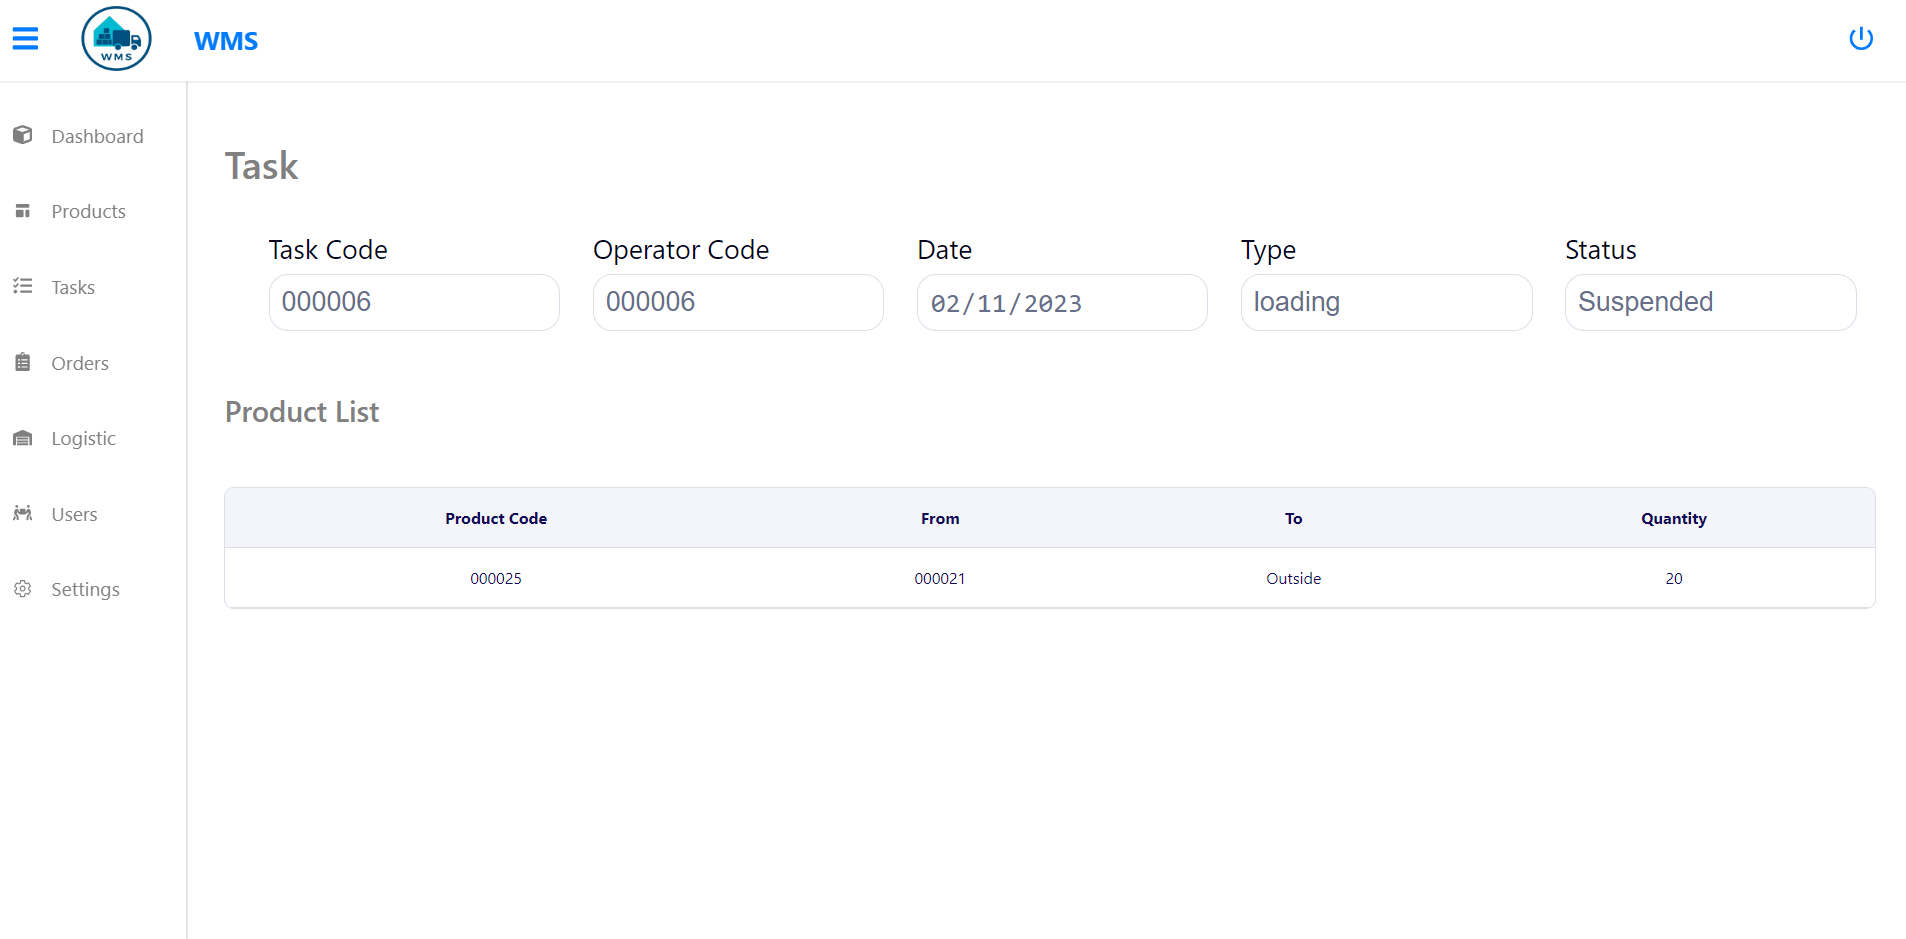
\includegraphics[width=\textwidth]{document/sections/img/Storyboard/viewTask.png}
    \caption{Task Page}
    \label{fig:viewTasksPage}
\end{figure}

Cliccando sull'icona \textbf{view} di un determinato task, l’admin viene
reindirizzato alla pagina di visualizzazione dei dettagli del task selezionato.\\
Questa pagina offre una visualizzazione tabellare, mostrando informazioni chiave per ogni prodotto
incluso nel task.

\begin{figure}[H]
    \centering
    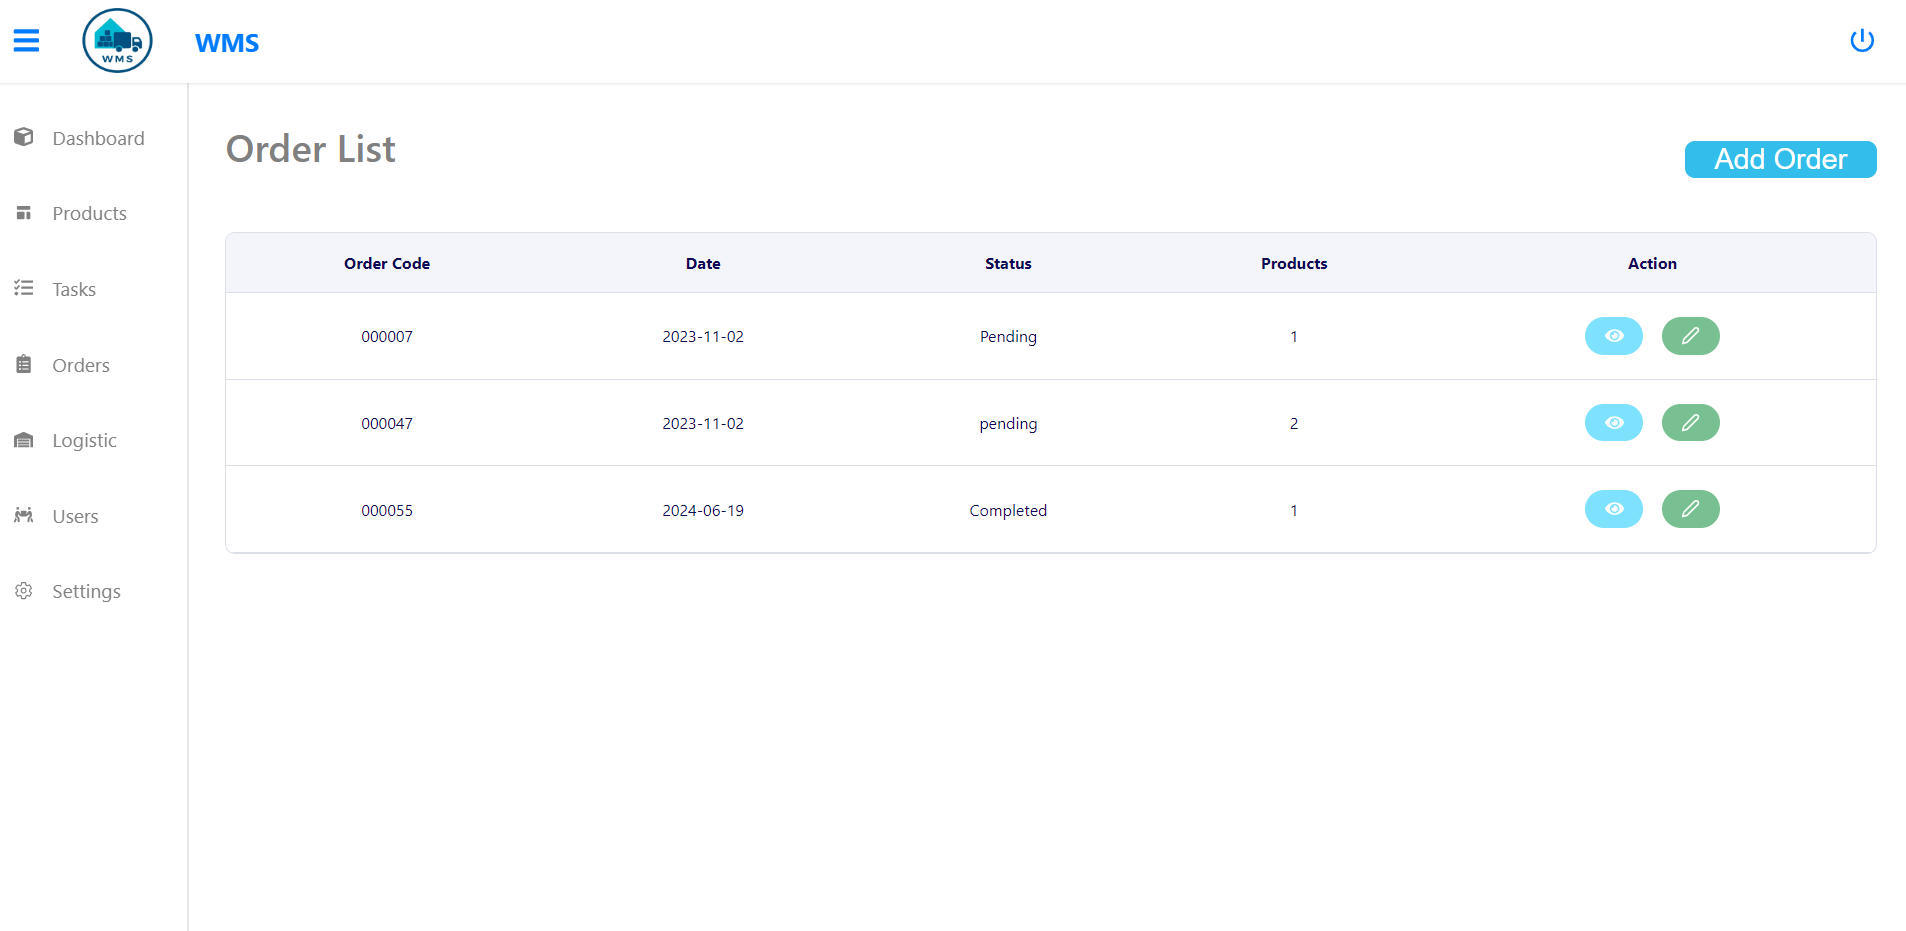
\includegraphics[width=\textwidth]{document/sections/img/Storyboard/orderPage.png}
    \caption{Orders Page}
    \label{fig:ordersPage}
\end{figure}

Cliccando sulla voce \textbf{Orders} nella sidebar, l'utente viene reindirizzato alla pagina di gestione degli ordini.\\
Questa pagina offre una visualizzazione tabellare degli ordini effettuati,
mostrando le informazioni chiave per ogni ordine.\\
Nella colonna di destra, sono presenti delle icone che consento di modificare, eliminare oppure visualizzare meglio
i dati di un singolo ordine.\\
In alto a destra è presente un pulsante \textbf{Add Order} che consente di aggiungere un nuovo ordine al sistema.

\begin{figure}[H]
    \centering
    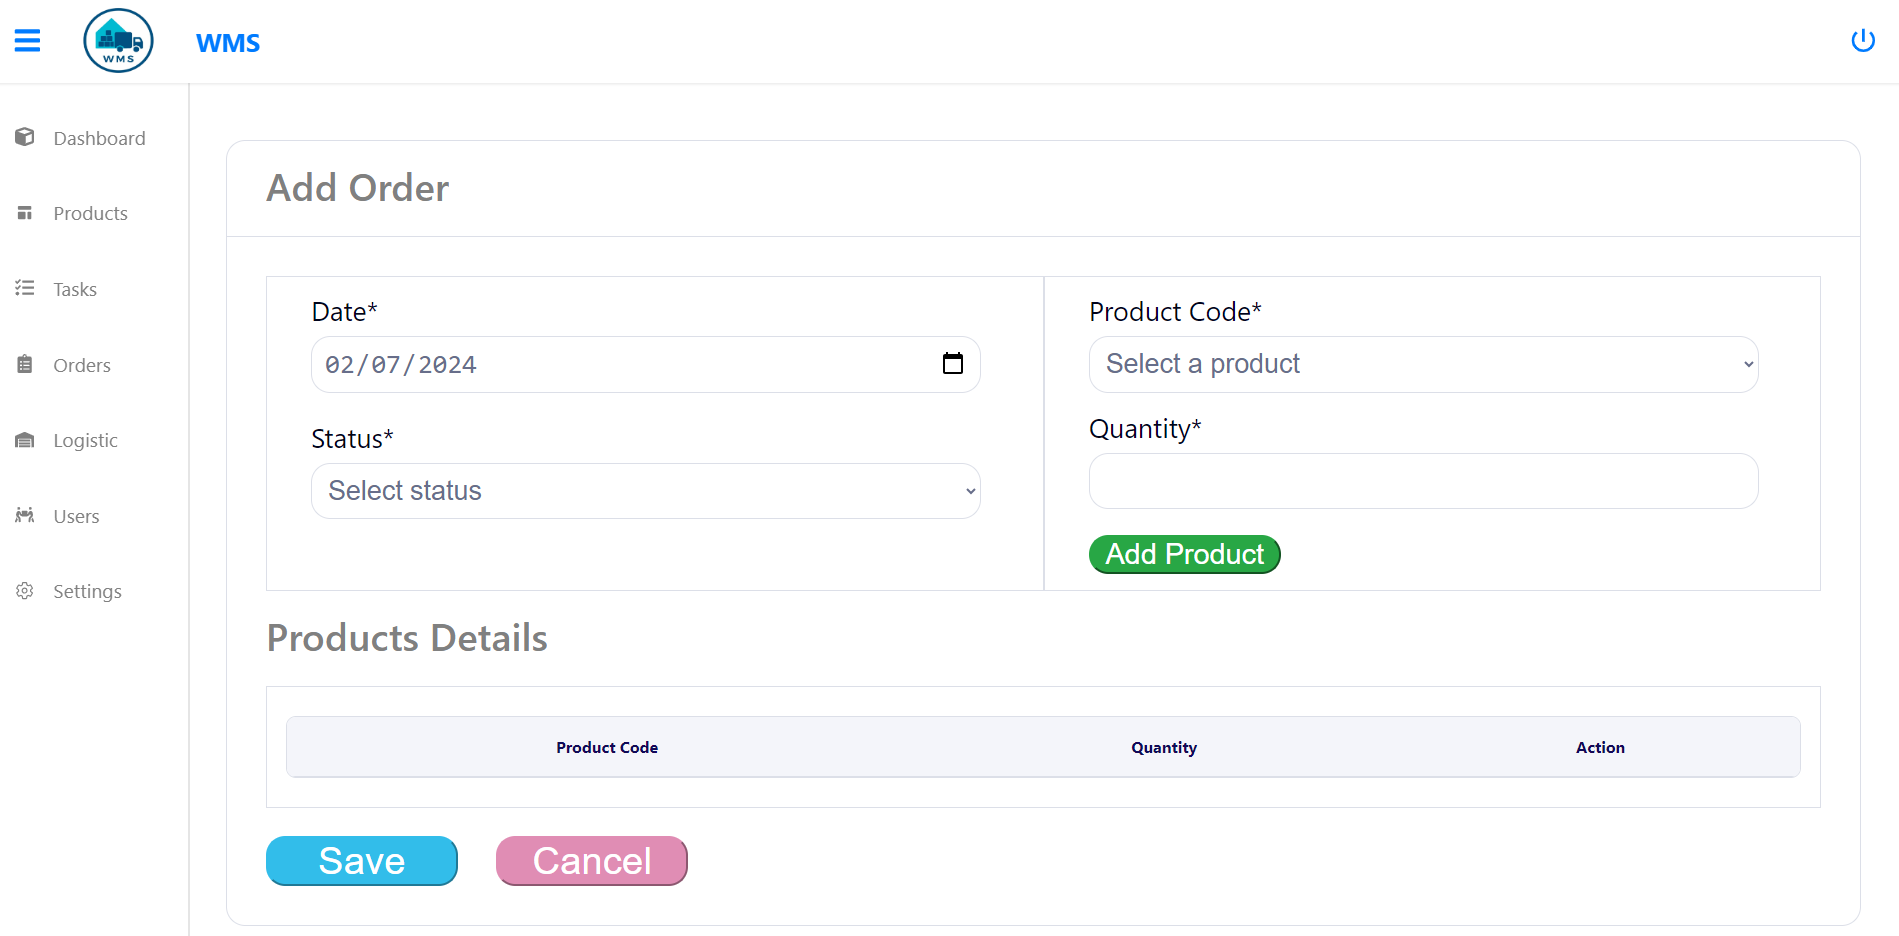
\includegraphics[width=\textwidth]{document/sections/img/Storyboard/addOrderPage.png}
    \caption{Add Order Page}
    \label{fig:addOrderPages}
\end{figure}

Cliccando sul pulsante \textbf{Add new} nella order page si apre un form, che consente
all'Admin di poter creare un nuovo ordine.\\
Sotto il form, è presente una sezione denominata \textbf{Products Details} che mostra i dettagli dei prodotti inclusi
nell'ordine in formato tabellare.\\
L'admin può  aggiungere più prodotti all'ordine utilizzando il pulsante \textbf{Add Product}.\\
Infine, in basso, sono presenti i pulsanti \textbf{Save} per salvare l'ordine e \textbf{Cancel} per annullare l'operazione
e tornare alla order page.
Qualora non venissero inseriti correttamente tutti i dati verrà mostrato un messaggio di errore.

\begin{figure}[H]
    \centering
    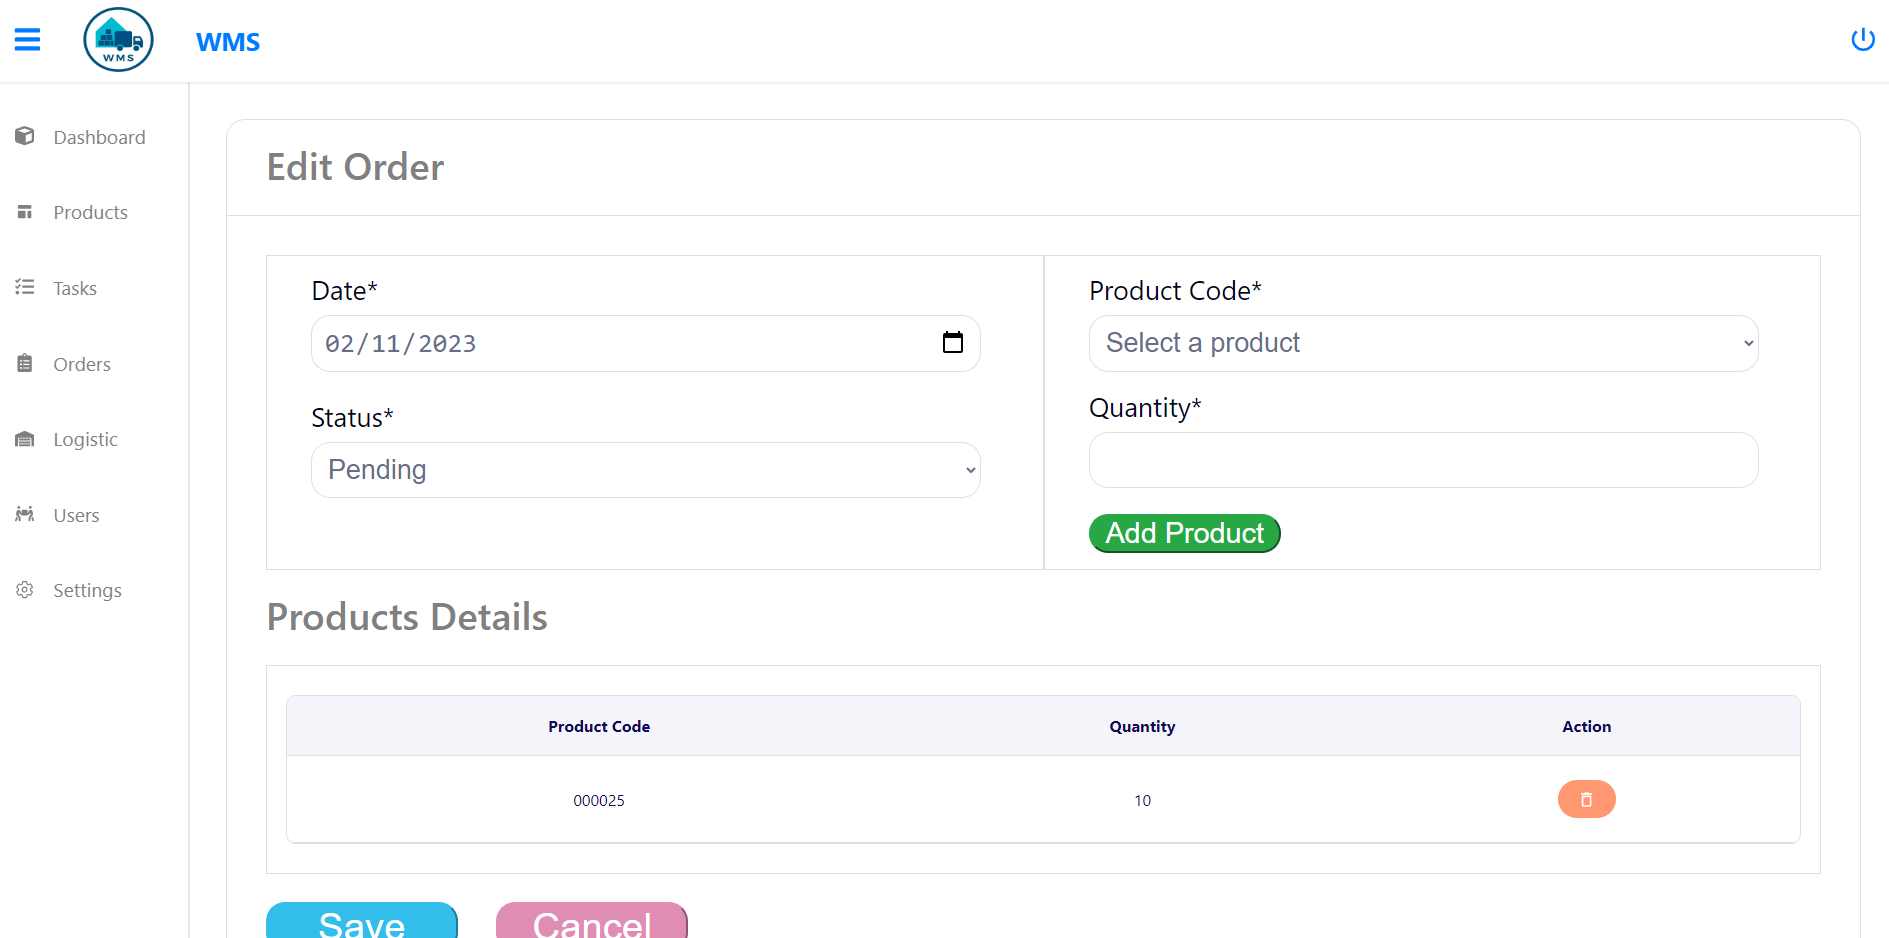
\includegraphics[width=\textwidth]{document/sections/img/Storyboard/editOrderPage.png}
    \caption{Edit Order Page}
    \label{fig:editOrderPage}
\end{figure}

Cliccando sull'icona \textbf{edit} di un determinato ordine, nella order page, si apre un form simile a quello che
consente di aggiungere un nuovo ordine, che permette all'Admin di modificarne i dati.\\
Cliccando sul bottone \textbf{Save} vengono salvate le modifiche, mentre cliccando sul bottone \textbf{Cancel} si torna alla order page.

\begin{figure}[H]
    \centering
    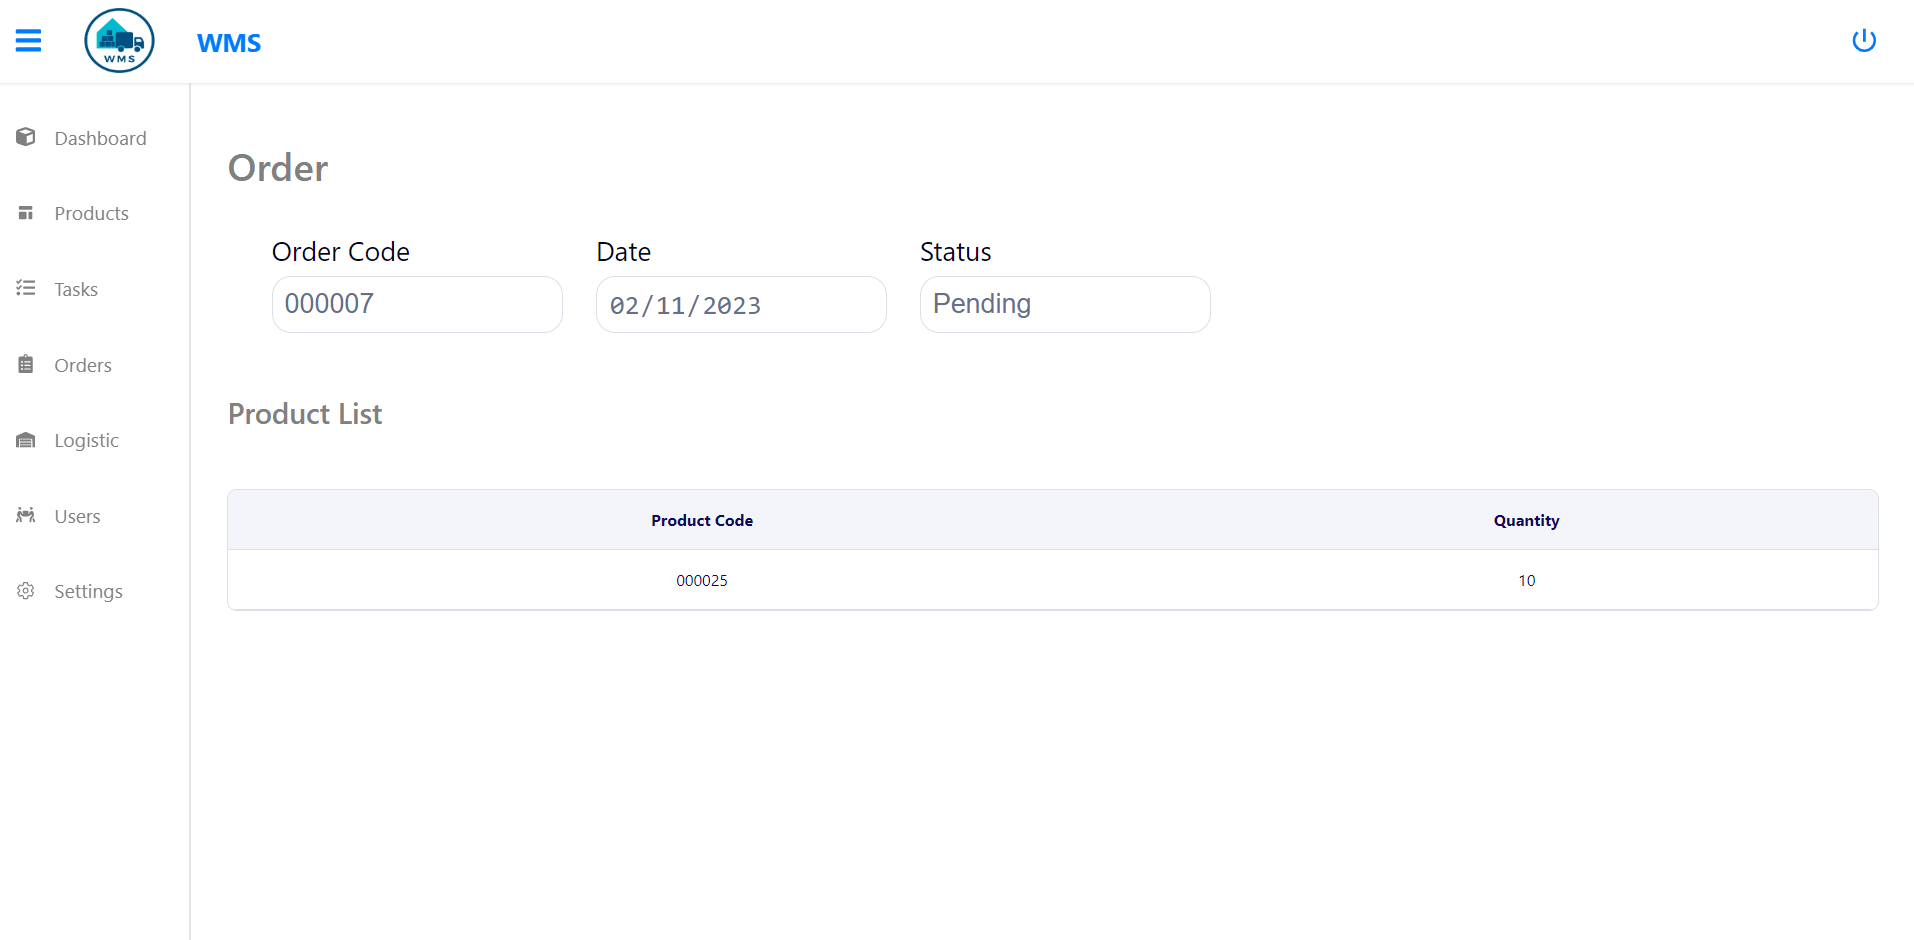
\includegraphics[width=\textwidth]{document/sections/img/Storyboard/viewOrder.png}
    \caption{Order Page}
    \label{fig:viewOrdersPage}
\end{figure}

Cliccando sull'icona \textbf{view} di un determinato ordine, l’admin viene
reindirizzato alla pagina di visualizzazione dei dettagli dell'ordine selezionato.\\
Questa pagina offre una visualizzazione tabellare, mostrando informazioni chiave per ogni prodotto
incluso nell'ordine.

\begin{figure}[H]
    \centering
    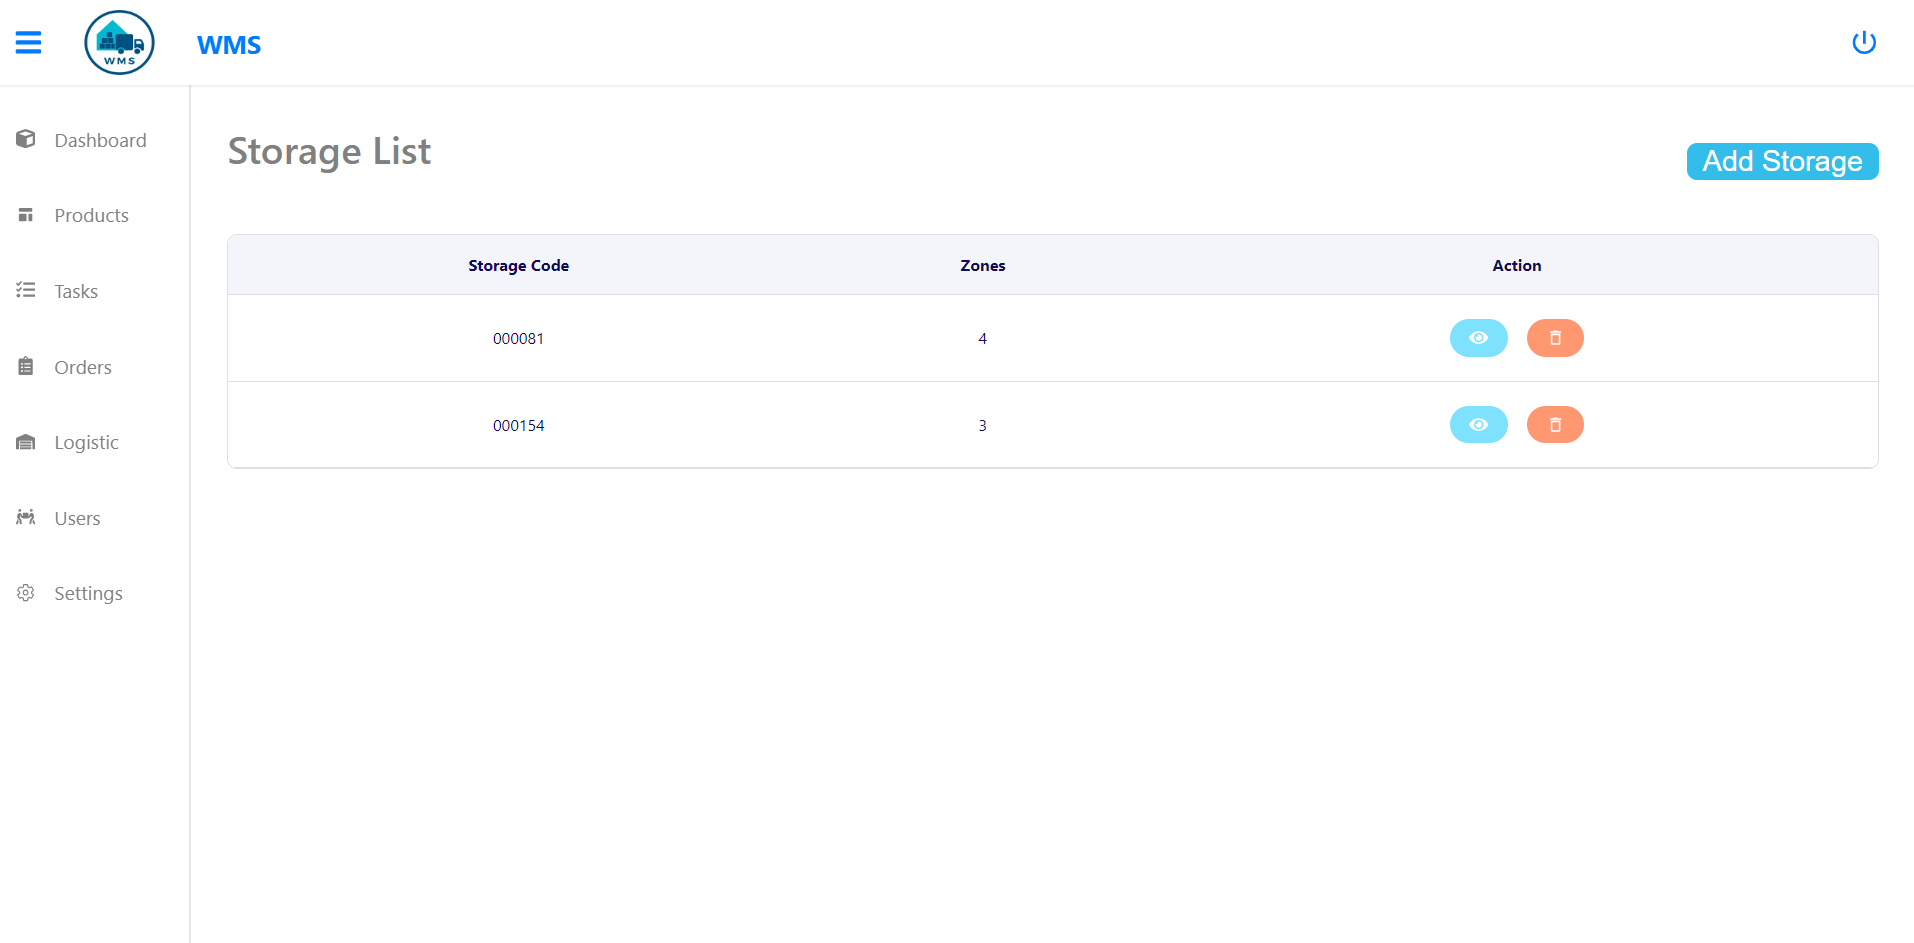
\includegraphics[width=\textwidth]{document/sections/img/Storyboard/storagePage.png}
    \caption{Storages Page}
    \label{fig:storagesPage}
\end{figure}

Cliccando sulla voce \textbf{Logistic} nella sidebar, l'utente viene reindirizzato alla pagina di gestione del magazzino.\\
Questa pagina offre una visualizzazione tabellare di tutti gli storage presenti.\\
Nella colonna di destra, sono presenti delle icone che consento di eliminare oppure visualizzare in dettaglio
le zone di un singolo magazzino.\\
In alto a destra è presente un pulsante \textbf{Add Storage} che consente di aggiungere un nuovo storage al sistema.

\begin{figure}[H]
    \centering
    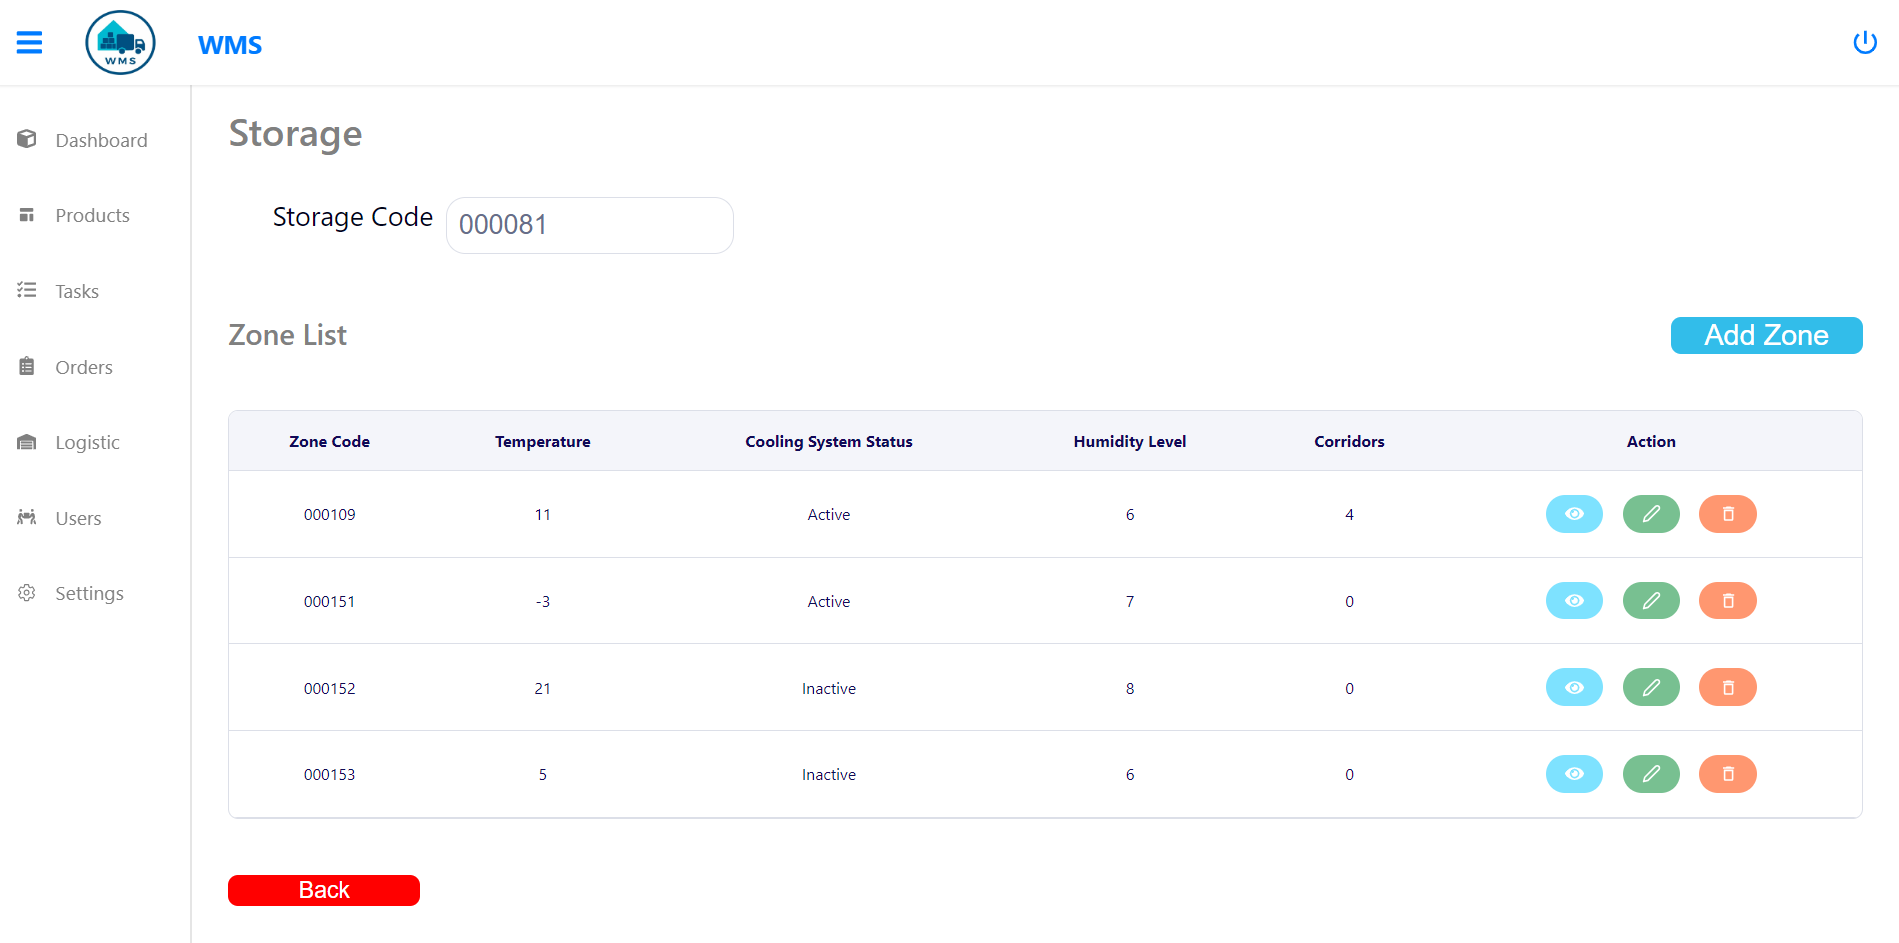
\includegraphics[width=\textwidth]{document/sections/img/Storyboard/viewStorage.png}
    \caption{Storage Page}
    \label{fig:storagePage}
\end{figure}

Cliccando sull'icona \textbf{view} di un determinato storage, l’admin viene
reindirizzato alla pagina di visualizzazione delle zone di cui è composto lo storage selezionato.\\
Inoltre la pagina mostra una lista delle zone in un formato tabellare. \\
In particolare, nella colonna di destra, sono presenti delle icone che consentono di modificare, eliminare oppure
visualizzare in dettaglio i dati di una singola zona.\\
In alto a destra è presente un pulsante \textbf{Add Zone} che consente di aggiungere nuove zone al magazzino.\\
In basso a sinistra è presente un pulsante \textbf{BACK} che consente di tornare alla storages page.

\begin{figure}[H]
    \centering
    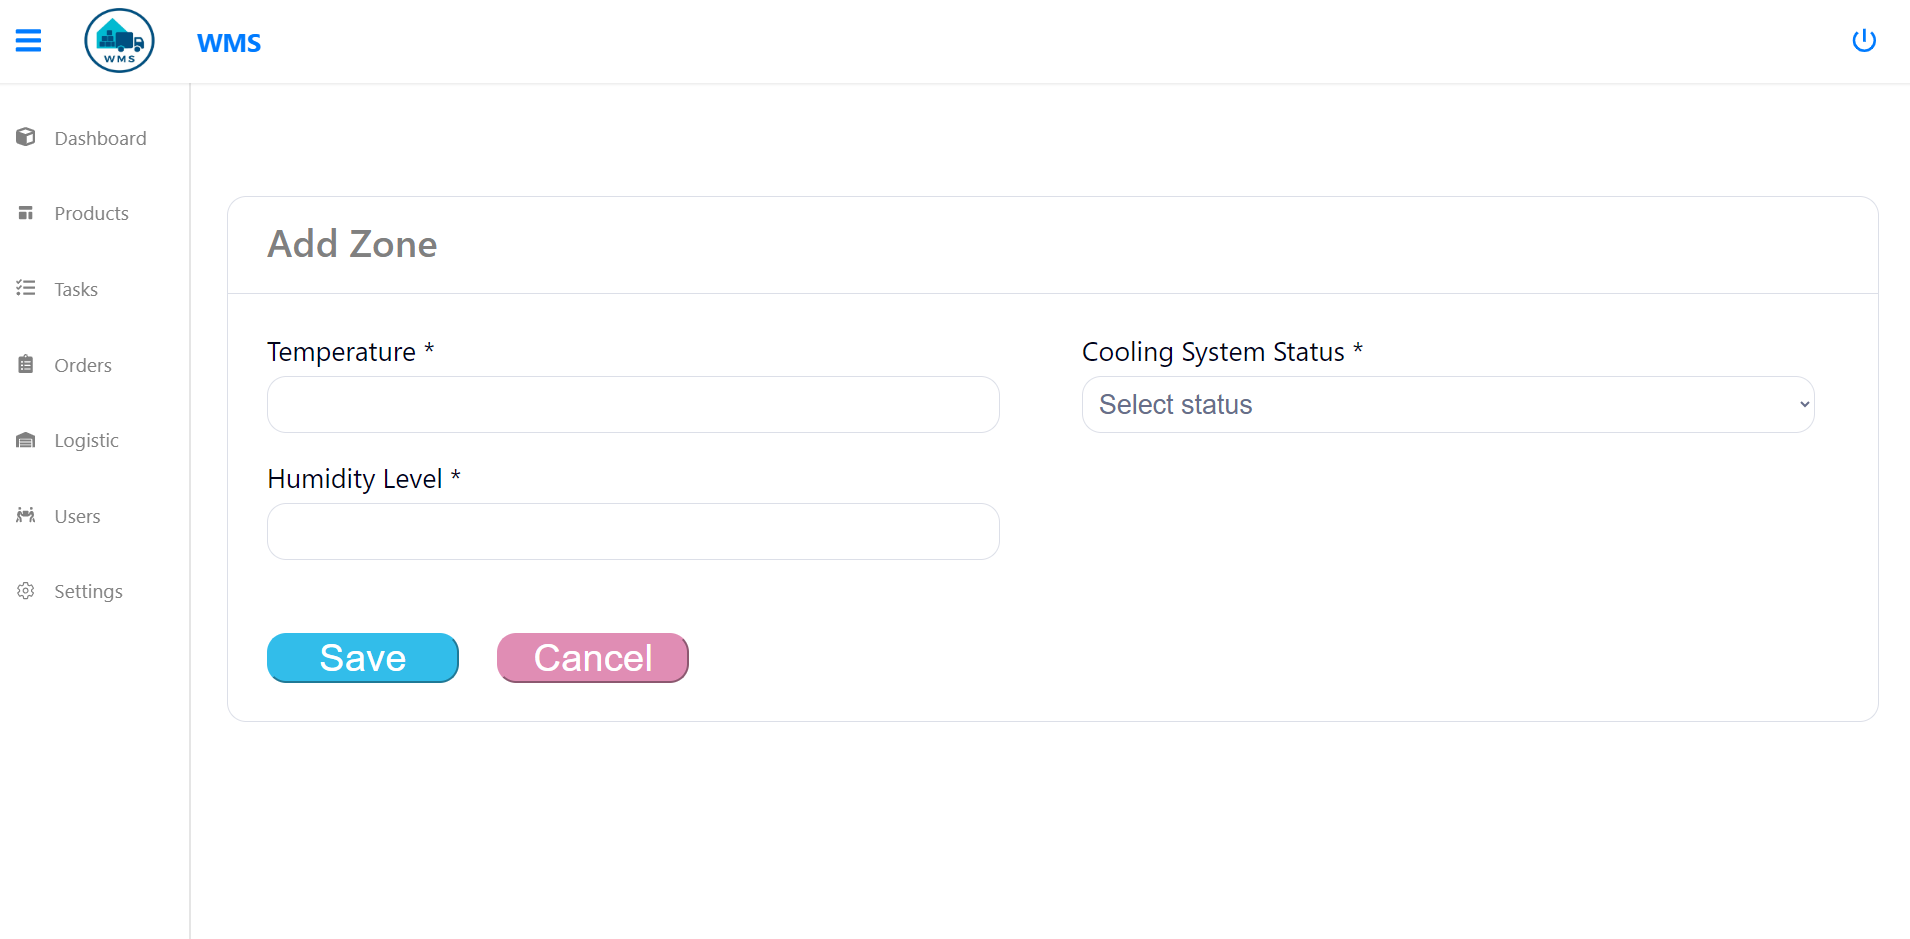
\includegraphics[width=\textwidth]{document/sections/img/Storyboard/addZone.png}
    \caption{Add Zone Page}
    \label{fig:addZonePages}
\end{figure}

Cliccando sul pulsante \textbf{Add new} nella storage page si apre un form, che consente
all'Admin di poter aggiungere una nuova zona allo storage.\\
In basso, sono presenti i pulsanti \textbf{Save} per salvare la zona e \textbf{Cancel} per annullare l'operazione
e tornare alla storage page.\\
Qualora non venissero inseriti correttamente tutti i dati verrà mostrato un messaggio di errore.

\begin{figure}[H]
    \centering
    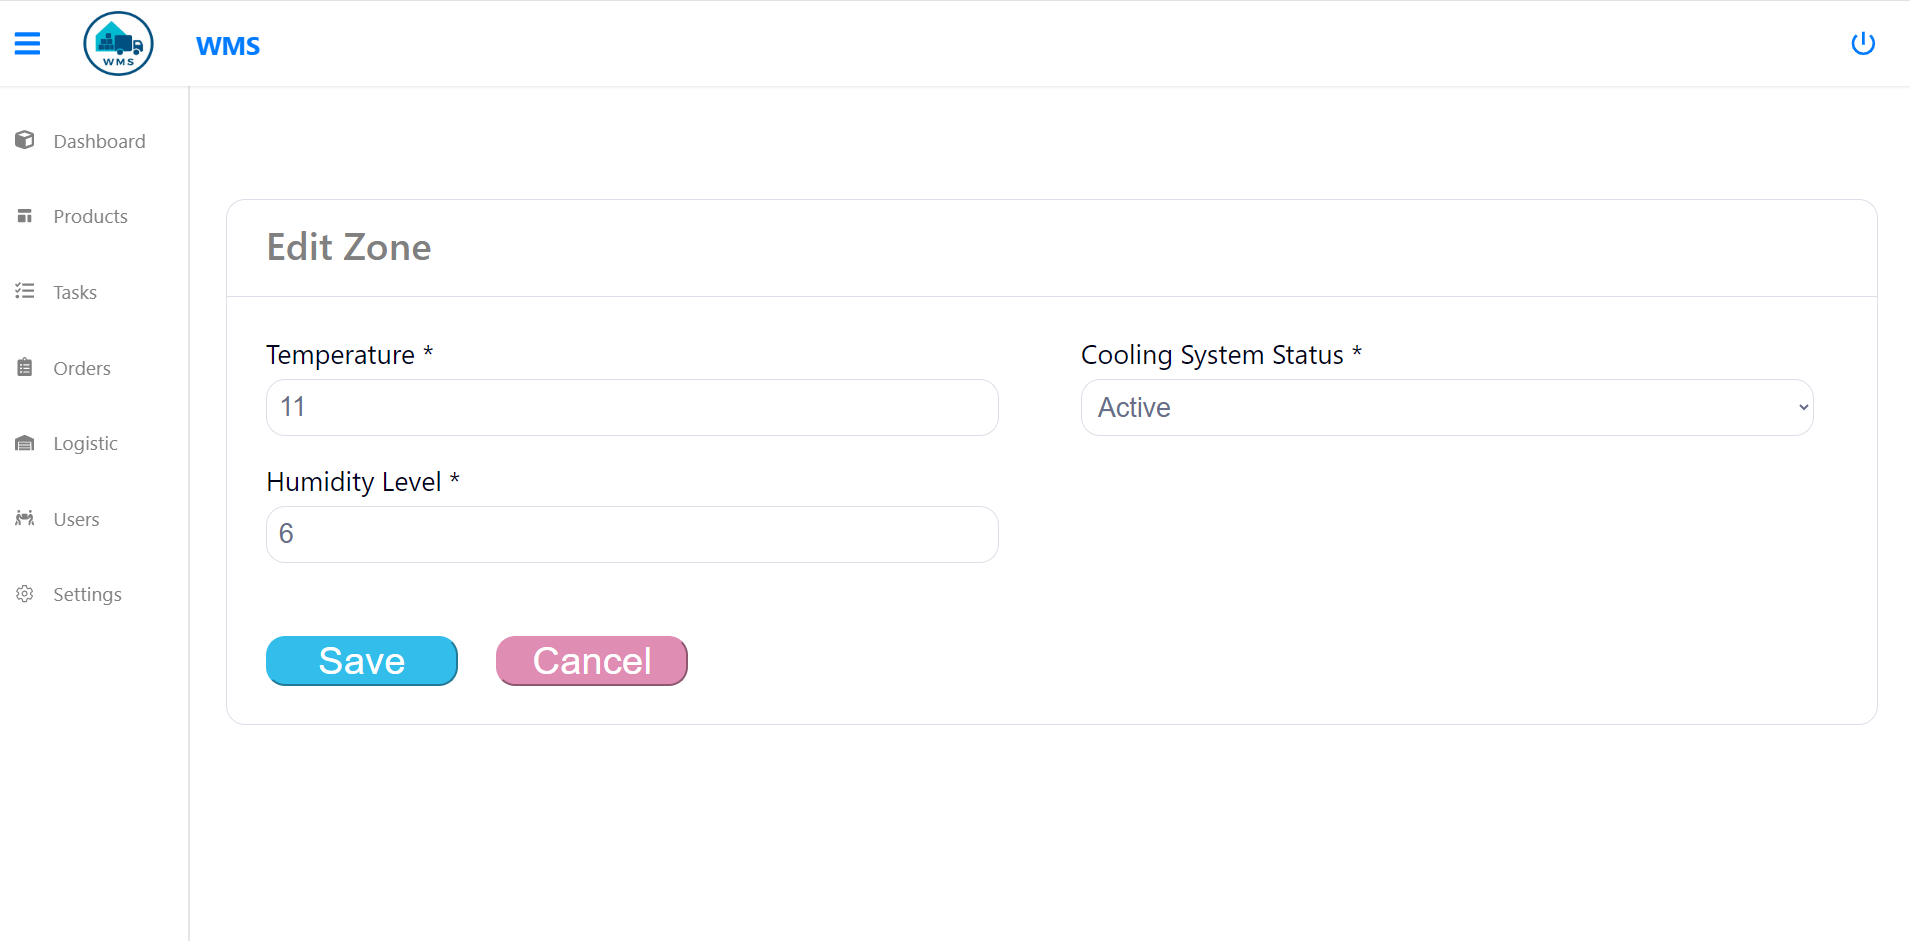
\includegraphics[width=\textwidth]{document/sections/img/Storyboard/editZonePage.png}
    \caption{Edit Zone Page}
    \label{fig:editZonePage}
\end{figure}

Cliccando sull'icona \textbf{edit} di una determinata zona, nella storage page, si apre un form
che permette all'Admin di poter modificare i dettagli di quest'ultima.\\
Cliccando sul bottone \textbf{Save} vengono salvate le modifiche, mentre cliccando sul bottone \textbf{Cancel} si torna alla storage page.

\begin{figure}[H]
    \centering
    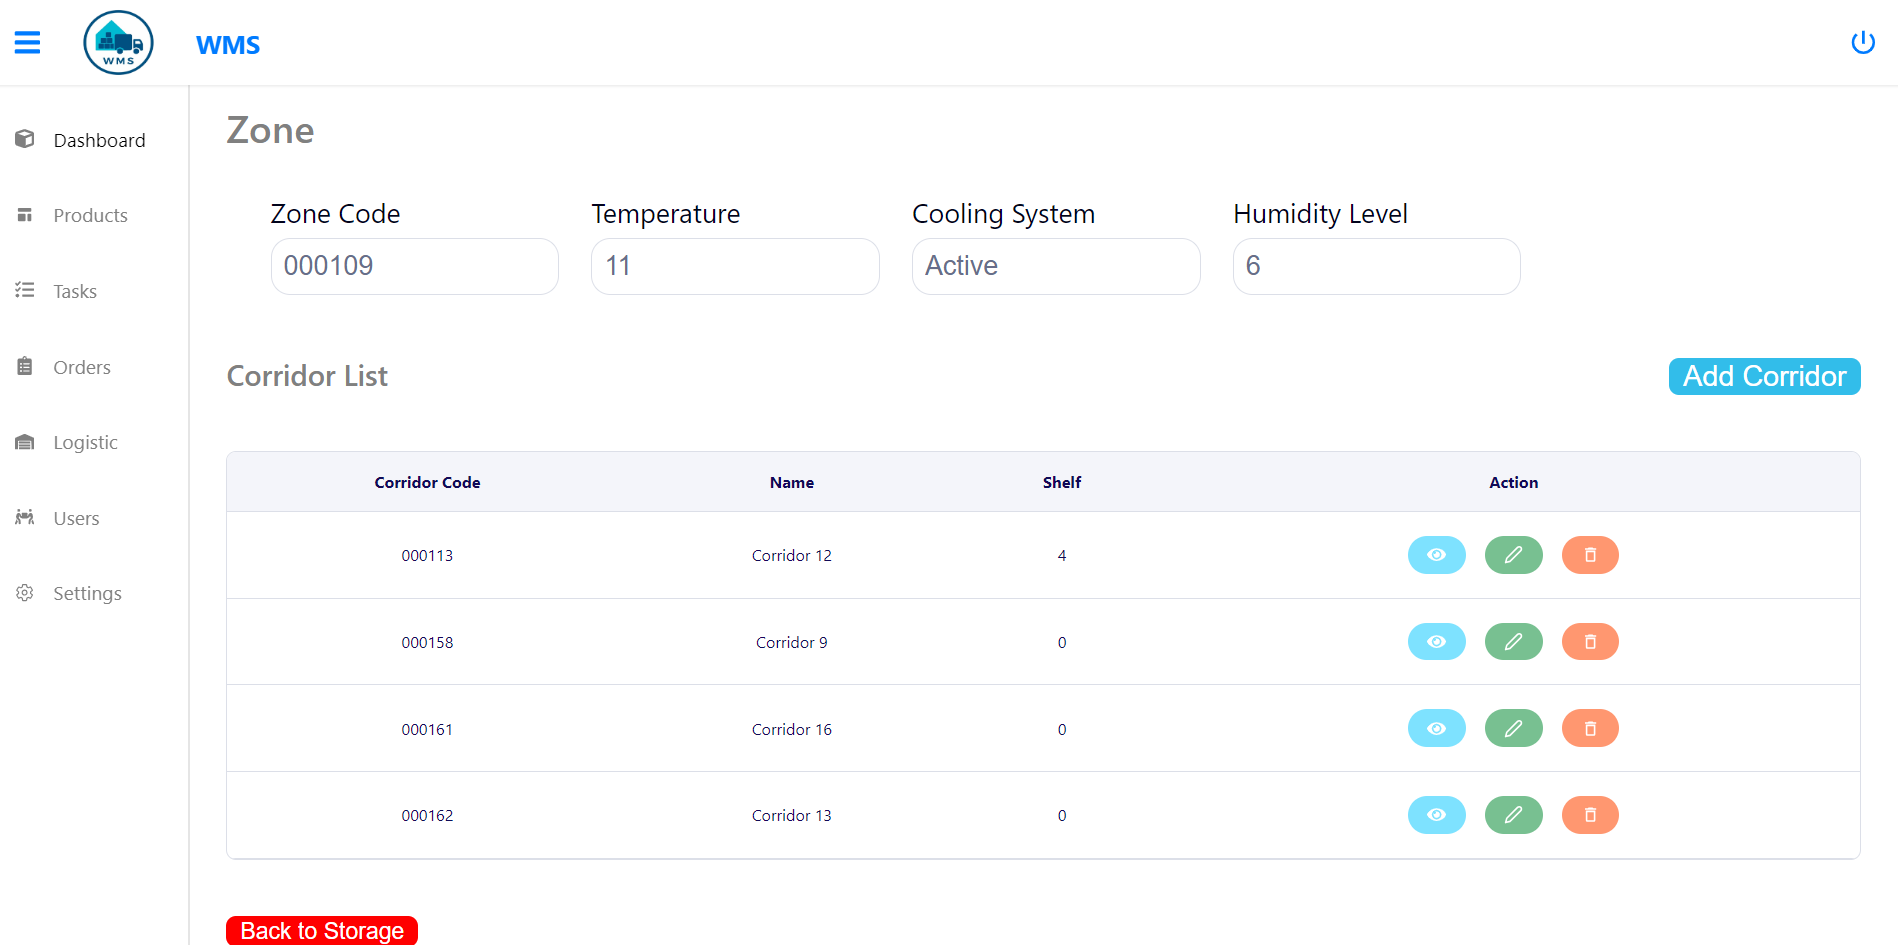
\includegraphics[width=\textwidth]{document/sections/img/Storyboard/viewZone.png}
    \caption{Zone Page}
    \label{fig:zonePage}
\end{figure}

Cliccando sull'icona \textbf{view} di una determinata zona nella pagina di gestione degli storage, l’admin viene reindirizzato alla pagina di visualizzazione dei dati della zona selezionata e dei corridoi che la compongono.\\
Questa pagina presenta una lista dei corridoi in formato tabellare.\\
Nella colonna di destra sono presenti icone che permettono di modificare, eliminare o visualizzare in dettaglio i dati di ciascun corridoio.\\
In alto a destra è disponibile un pulsante \textbf{Add Corridor} per aggiungere un nuovo corridoio alla zona.\\
In basso a sinistra è presente il pulsante \textbf{Back to Storage} per tornare alla storage page.

\begin{figure}[H]
    \centering
    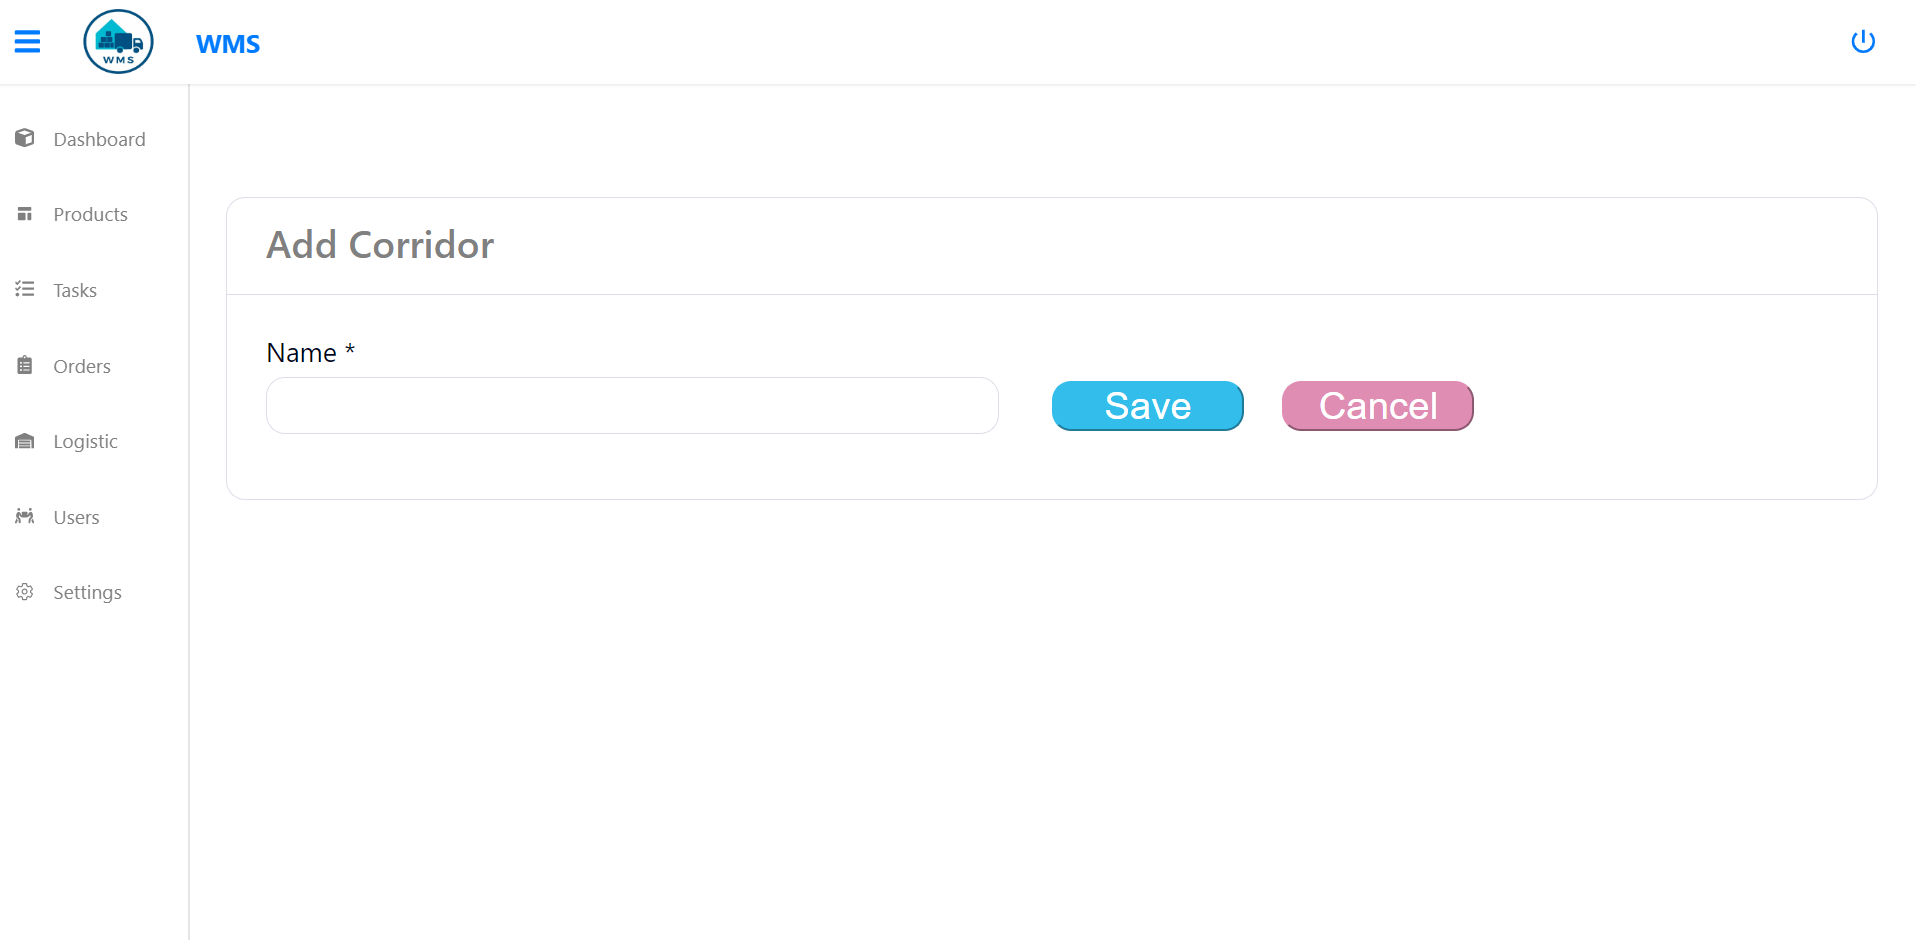
\includegraphics[width=\textwidth]{document/sections/img/Storyboard/addCorridorPage.png}
    \caption{Add Corridor Page}
    \label{fig:addCorridorPages}
\end{figure}

Cliccando sul pulsante \textbf{Add new} nella zone page si apre un form, che consente
all'Admin di poter aggiungere un nuovo corridoio alla zona.\\
In basso, sono presenti i pulsanti \textbf{Save} per salvare il corridoio e \textbf{Cancel} per annullare l'operazione
e tornare alla zone page.\\
Qualora non venissero inseriti correttamente tutti i dati verrà mostrato un messaggio di errore.

\begin{figure}[H]
    \centering
    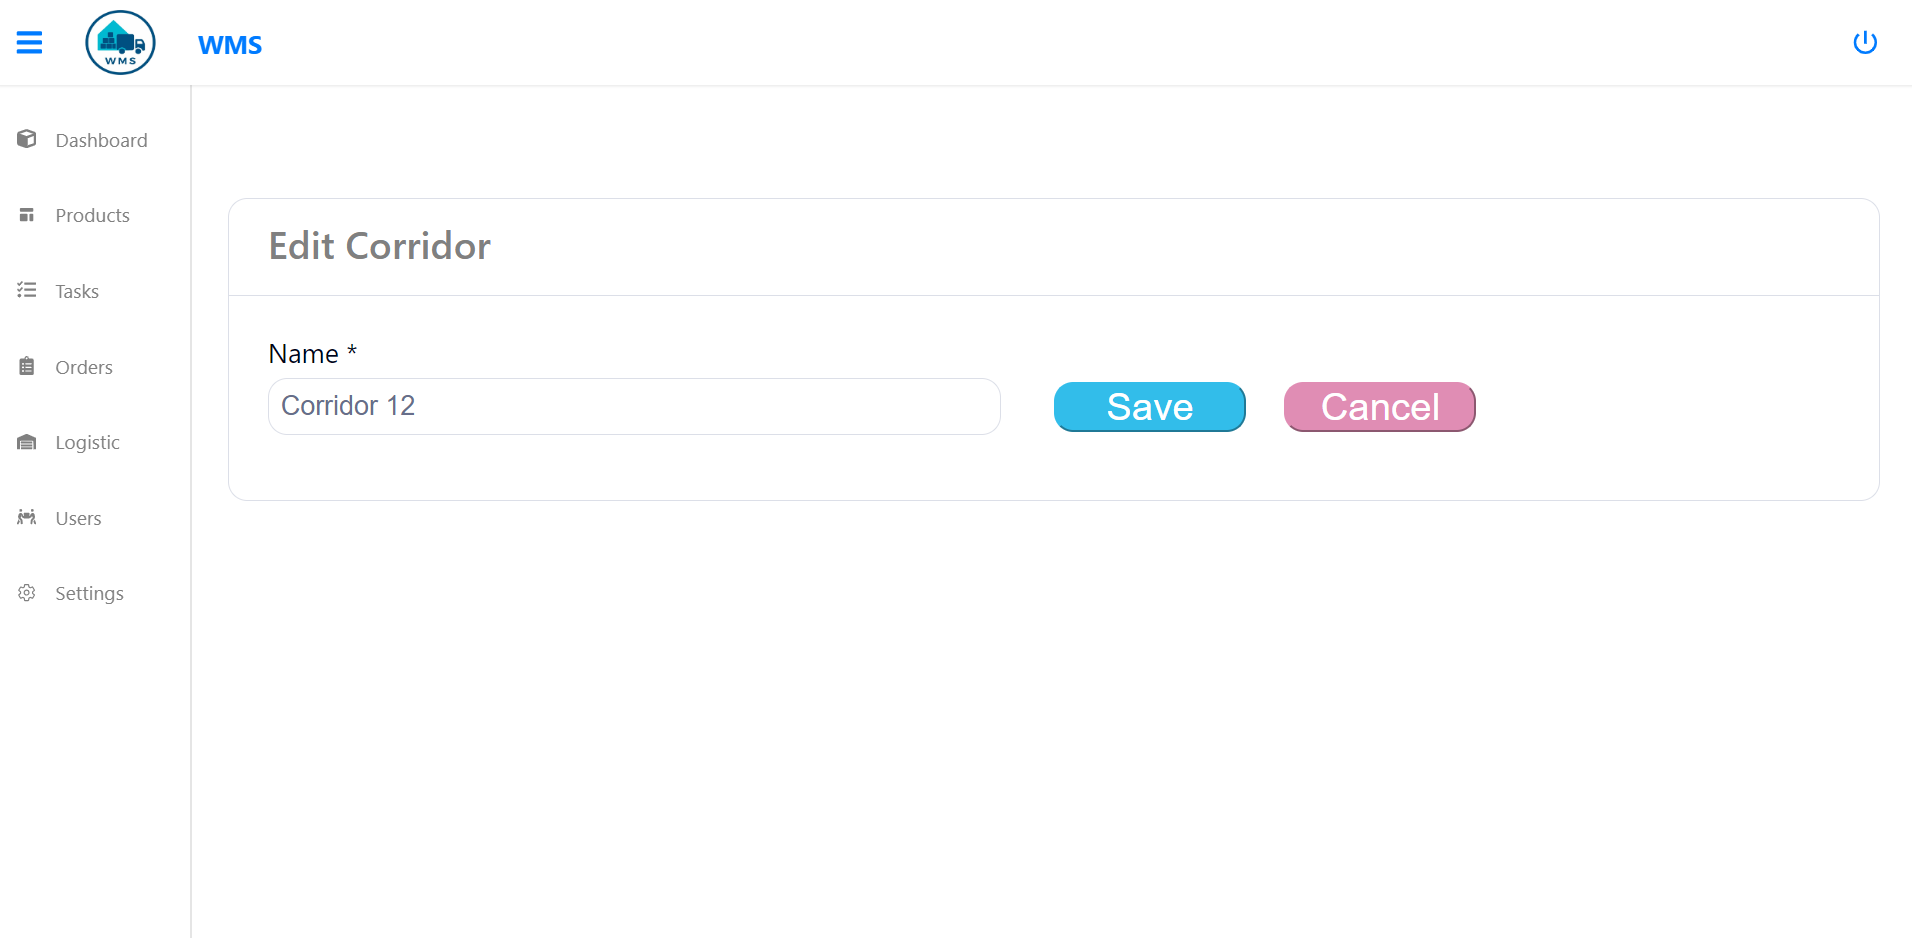
\includegraphics[width=\textwidth]{document/sections/img/Storyboard/editCorridorPage.png}
    \caption{Edit Corridor Page}
    \label{fig:editCorridorPage}
\end{figure}

Cliccando sull'icona \textbf{edit} di un determinato corridoio, nella zone page, si apre un form
che permette all'Admin di modificarne il nome.\\
Cliccando sul bottone \textbf{Save} vengono salvate le modifiche, mentre cliccando sul bottone \textbf{Cancel} si torna alla zone page.

\begin{figure}[H]
    \centering
    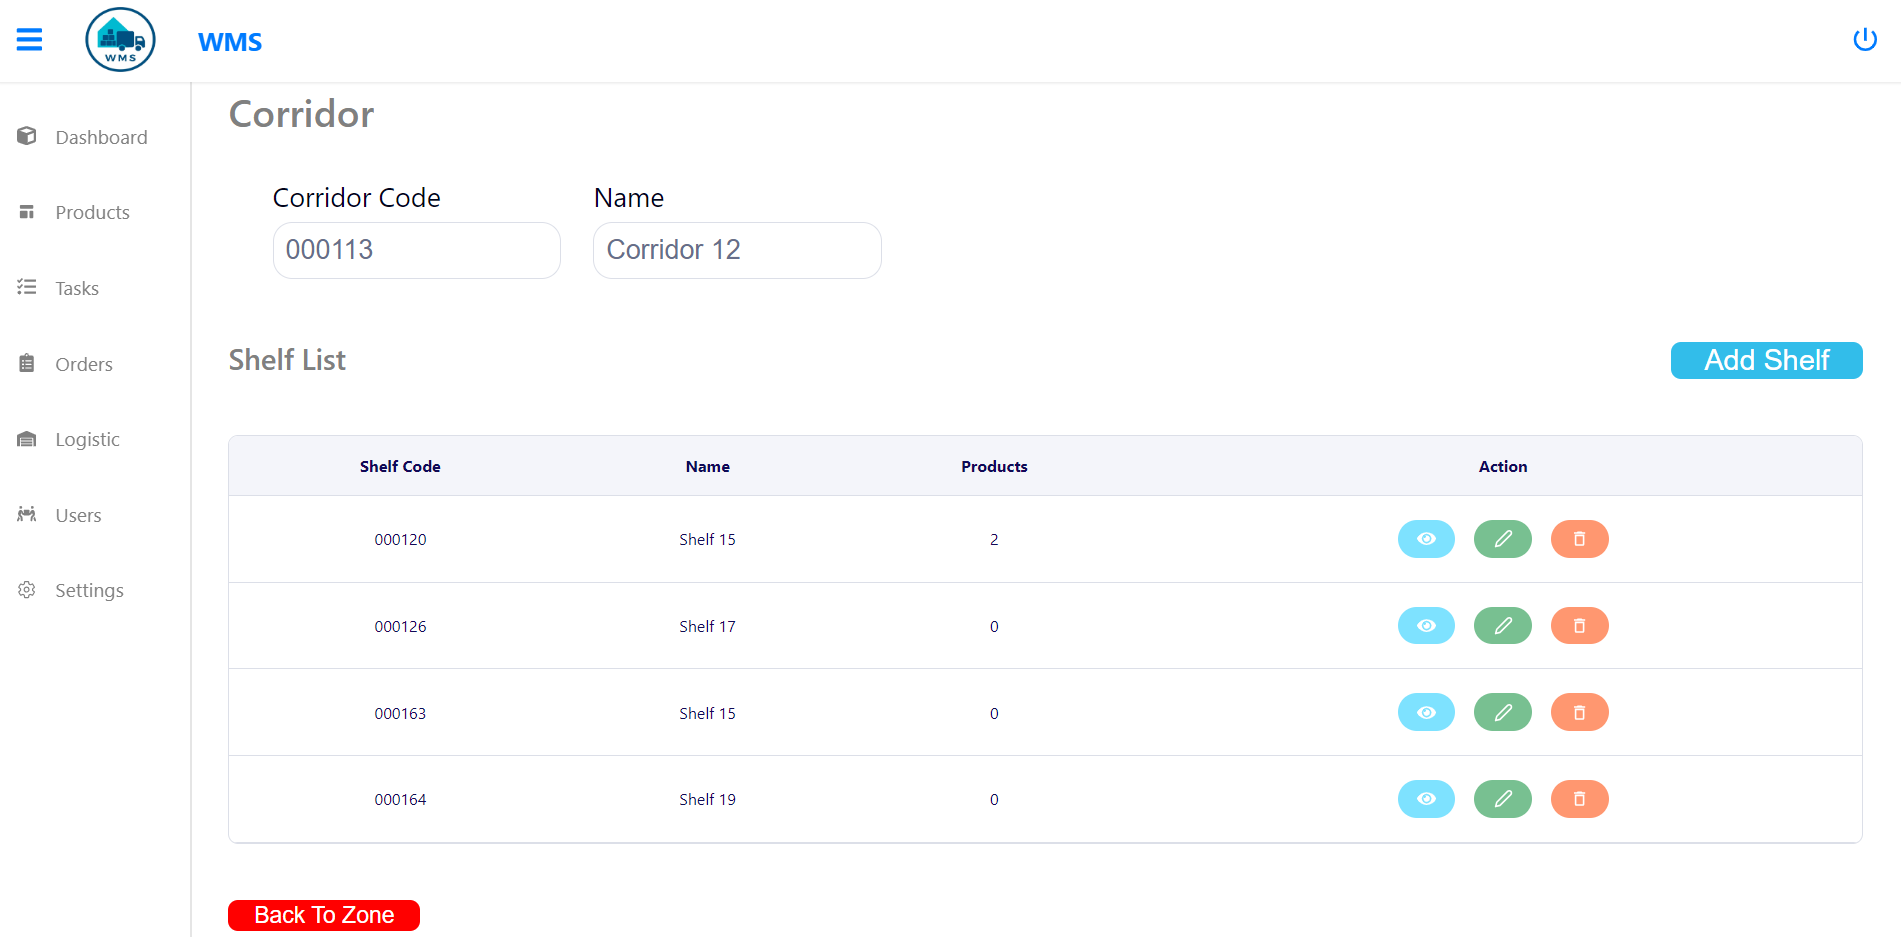
\includegraphics[width=\textwidth]{document/sections/img/Storyboard/viewCorridor.png}
    \caption{Corridor Page}
    \label{fig:corridorPage}
\end{figure}

Cliccando sull'icona \textbf{view} di un determinato corridoio nella pagina di gestione delle zone,
l’admin viene reindirizzato alla pagina di visualizzazione dei dati del corridoio selezionato e degli scaffali che la compongono.\\
Questa pagina presenta una lista degli scaffali in formato tabellare.\\
Nella colonna di destra sono presenti icone che permettono di modificare, eliminare o visualizzare in dettaglio i dati di ciascun scaffale.\\
In alto a destra è disponibile un pulsante \textbf{Add Shelf} per aggiungere un nuovo scaffale al corridoio.\\
In basso a sinistra è presente il pulsante \textbf{Back to Zone} per tornare alla zone page.

\begin{figure}[H]
    \centering
    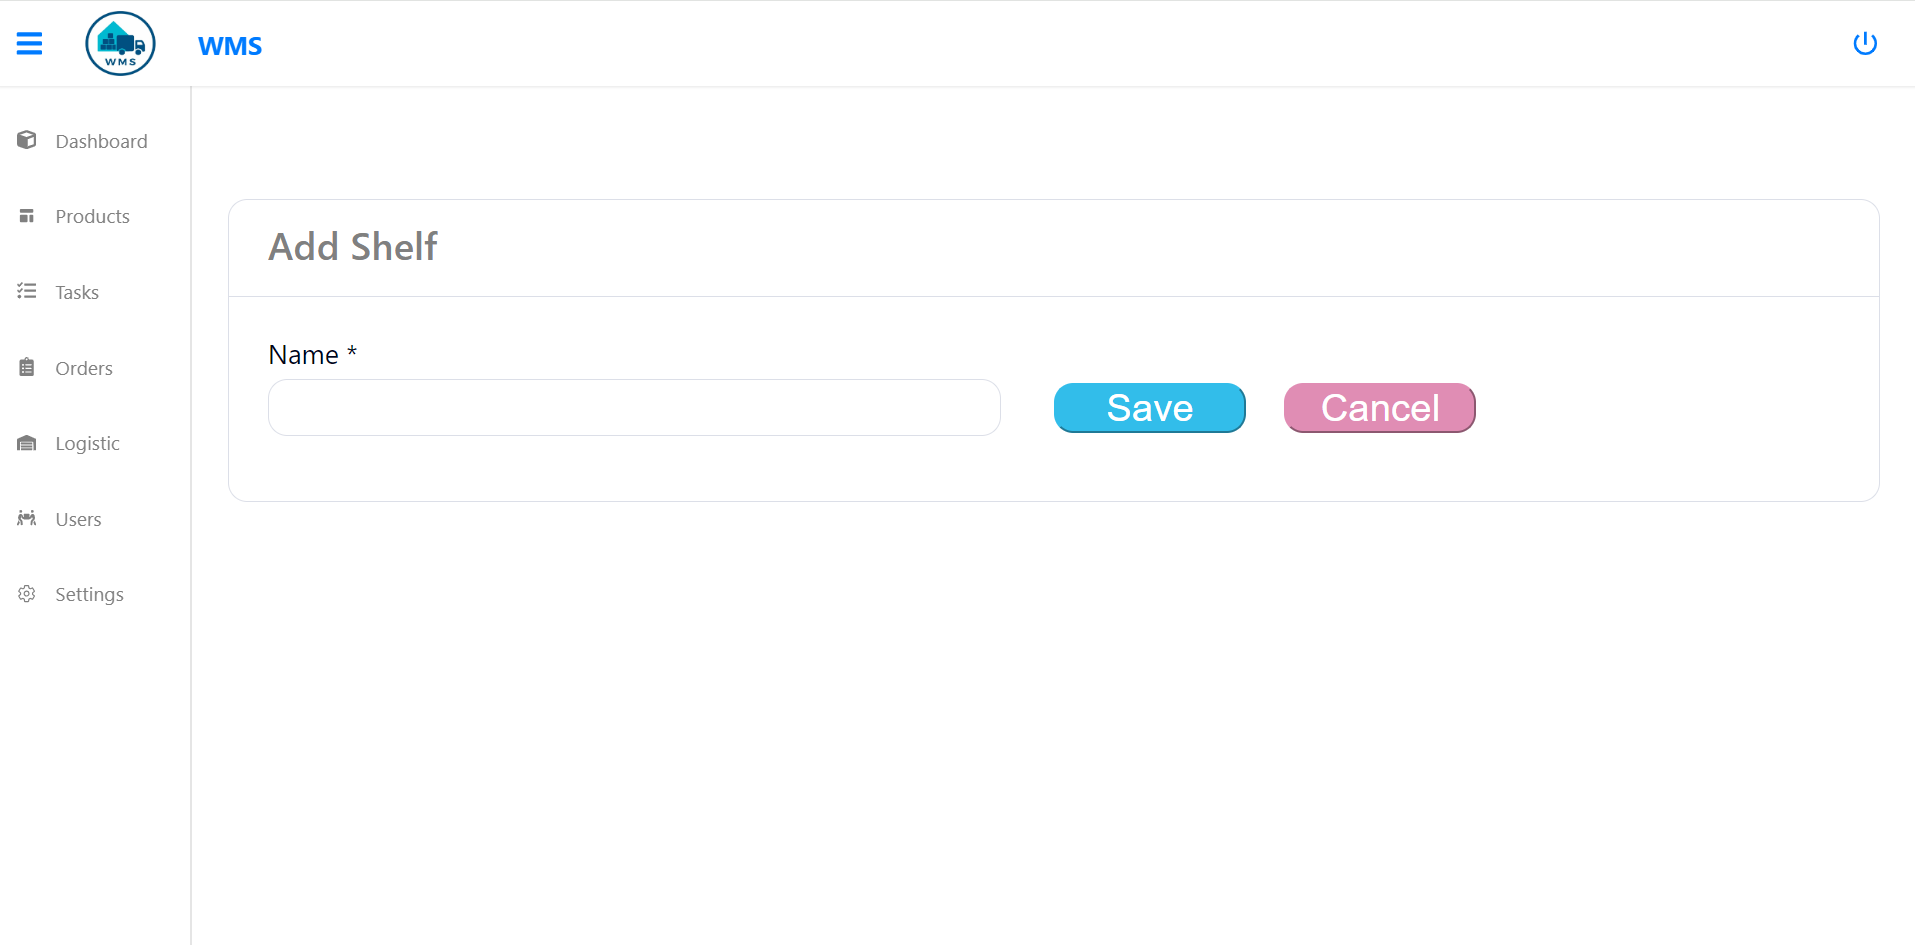
\includegraphics[width=\textwidth]{document/sections/img/Storyboard/addShelfPage.png}
    \caption{Add Shelf Page}
    \label{fig:addShelfPages}
\end{figure}

Cliccando sul pulsante \textbf{Add new} nella corridor page si apre un form, che consente
all'Admin di poter aggiungere un nuovo scaffale al corridoio.\\
In basso, sono presenti i pulsanti \textbf{Save} per salvare lo scaffale e \textbf{Cancel} per annullare l'operazione
e tornare alla corridor page.
Qualora non venissero inseriti correttamente tutti i dati verrà mostrato un messaggio di errore.

\begin{figure}[H]
    \centering
    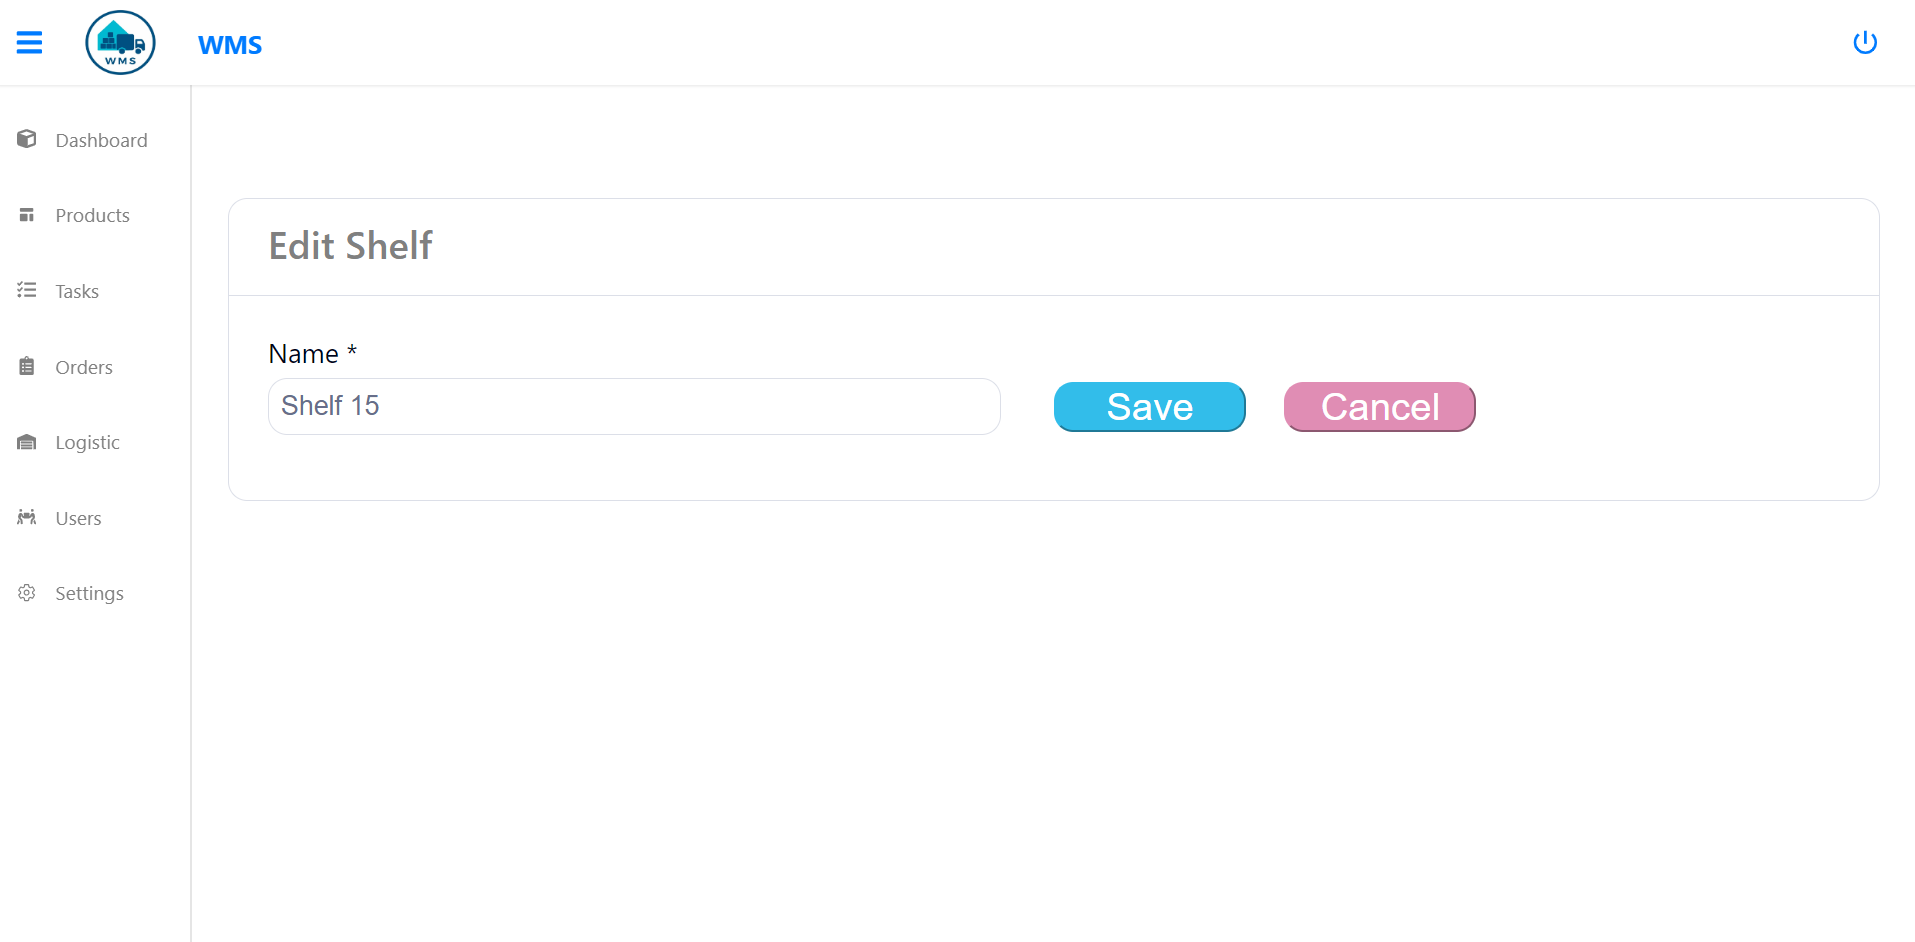
\includegraphics[width=\textwidth]{document/sections/img/Storyboard/editShelfPage.png}
    \caption{Edit Shelf Page}
    \label{fig:editShelfPage}
\end{figure}

Cliccando sull'icona \textbf{edit} di un determinato scaffale, nella corridor page, si apre un form
che permette all'Admin di modificarne il nome.\\
Cliccando sul bottone \textbf{Save} vengono salvate le modifiche, mentre cliccando sul bottone \textbf{Cancel} si torna alla corridor page.

\begin{figure}[H]
    \centering
    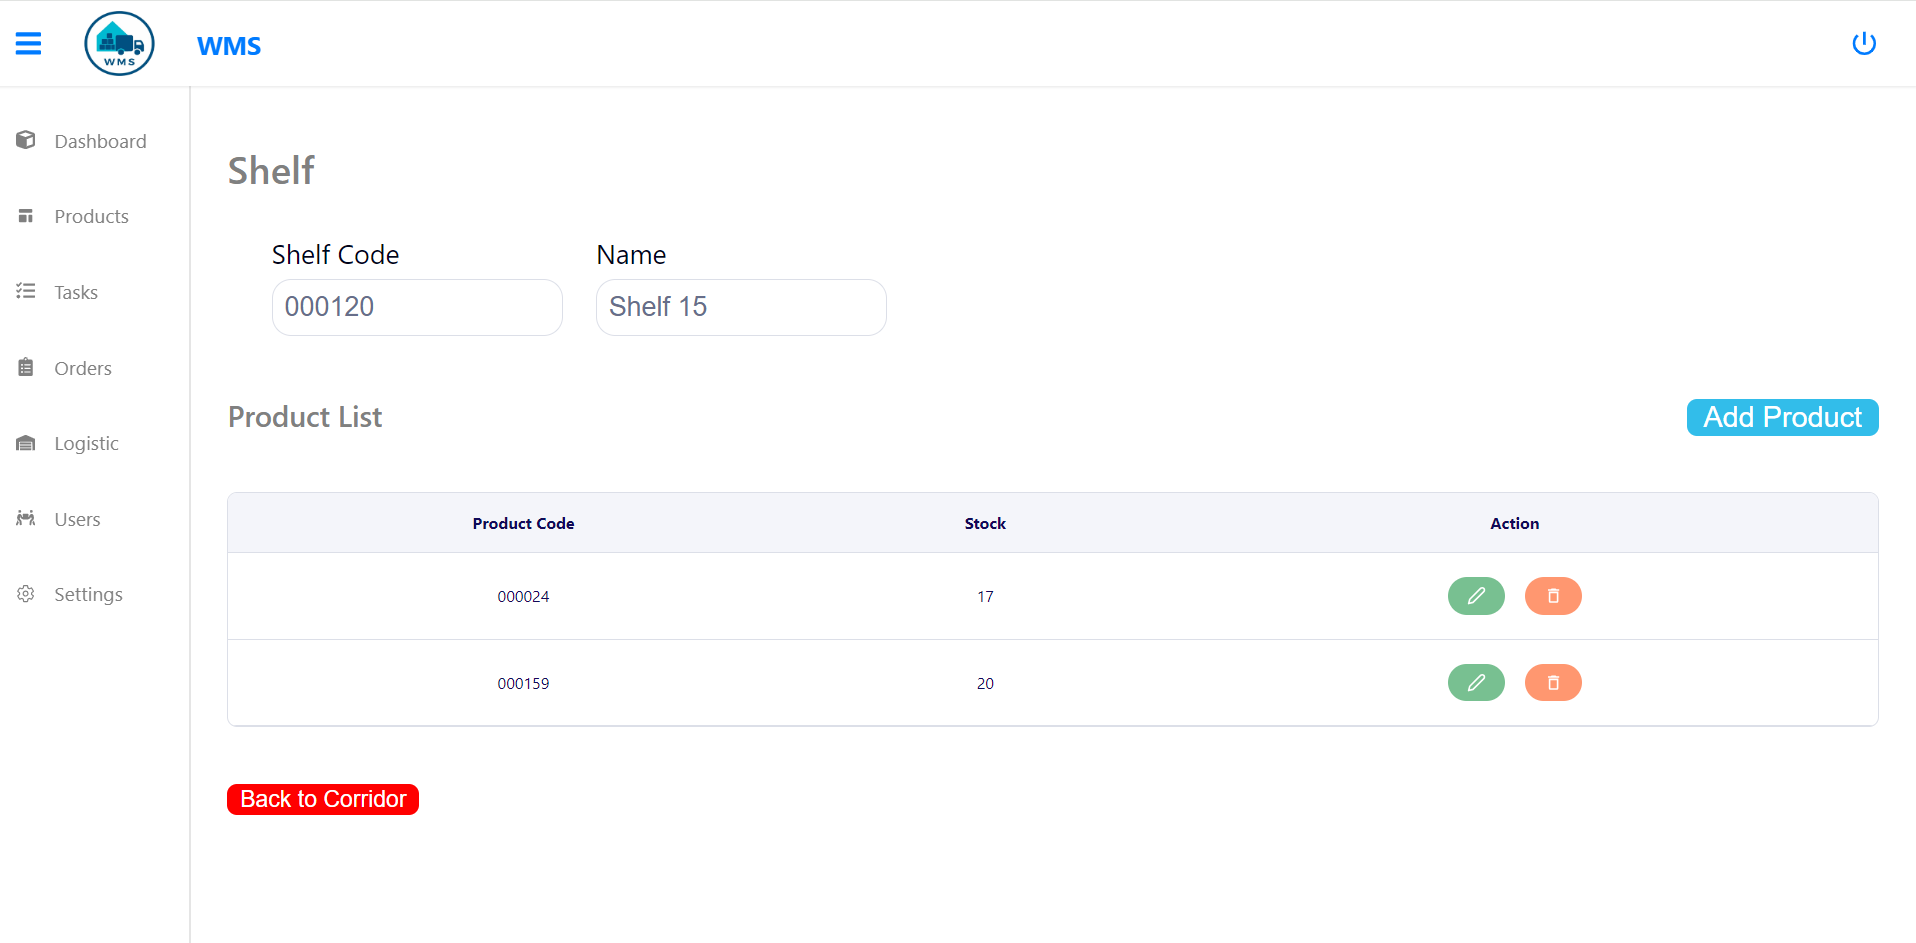
\includegraphics[width=\textwidth]{document/sections/img/Storyboard/viewShelf.png}
    \caption{Shelf Page}
    \label{fig:shelfPage}
\end{figure}

Cliccando sull'icona \textbf{view} di uno specifico scaffale nella pagina del corridoio, l'admin viene reindirizzato alla pagina di visualizzazione dei dati dello scaffale selezionato e dei prodotti presenti in esso.\\
Questa pagina mostra una lista dei prodotti in formato tabellare.\\
Nella colonna di destra sono presenti icone che permettono di modificare o eliminare i dati di ciascun prodotto.\\
In alto a destra è disponibile un pulsante \textbf{Add Product} per aggiungere un nuovo prodotto allo scaffale.\\
In basso a sinistra è presente il pulsante \textbf{Back to Corridor} per tornare alla pagina del corridoio.

\begin{figure}[H]
    \centering
    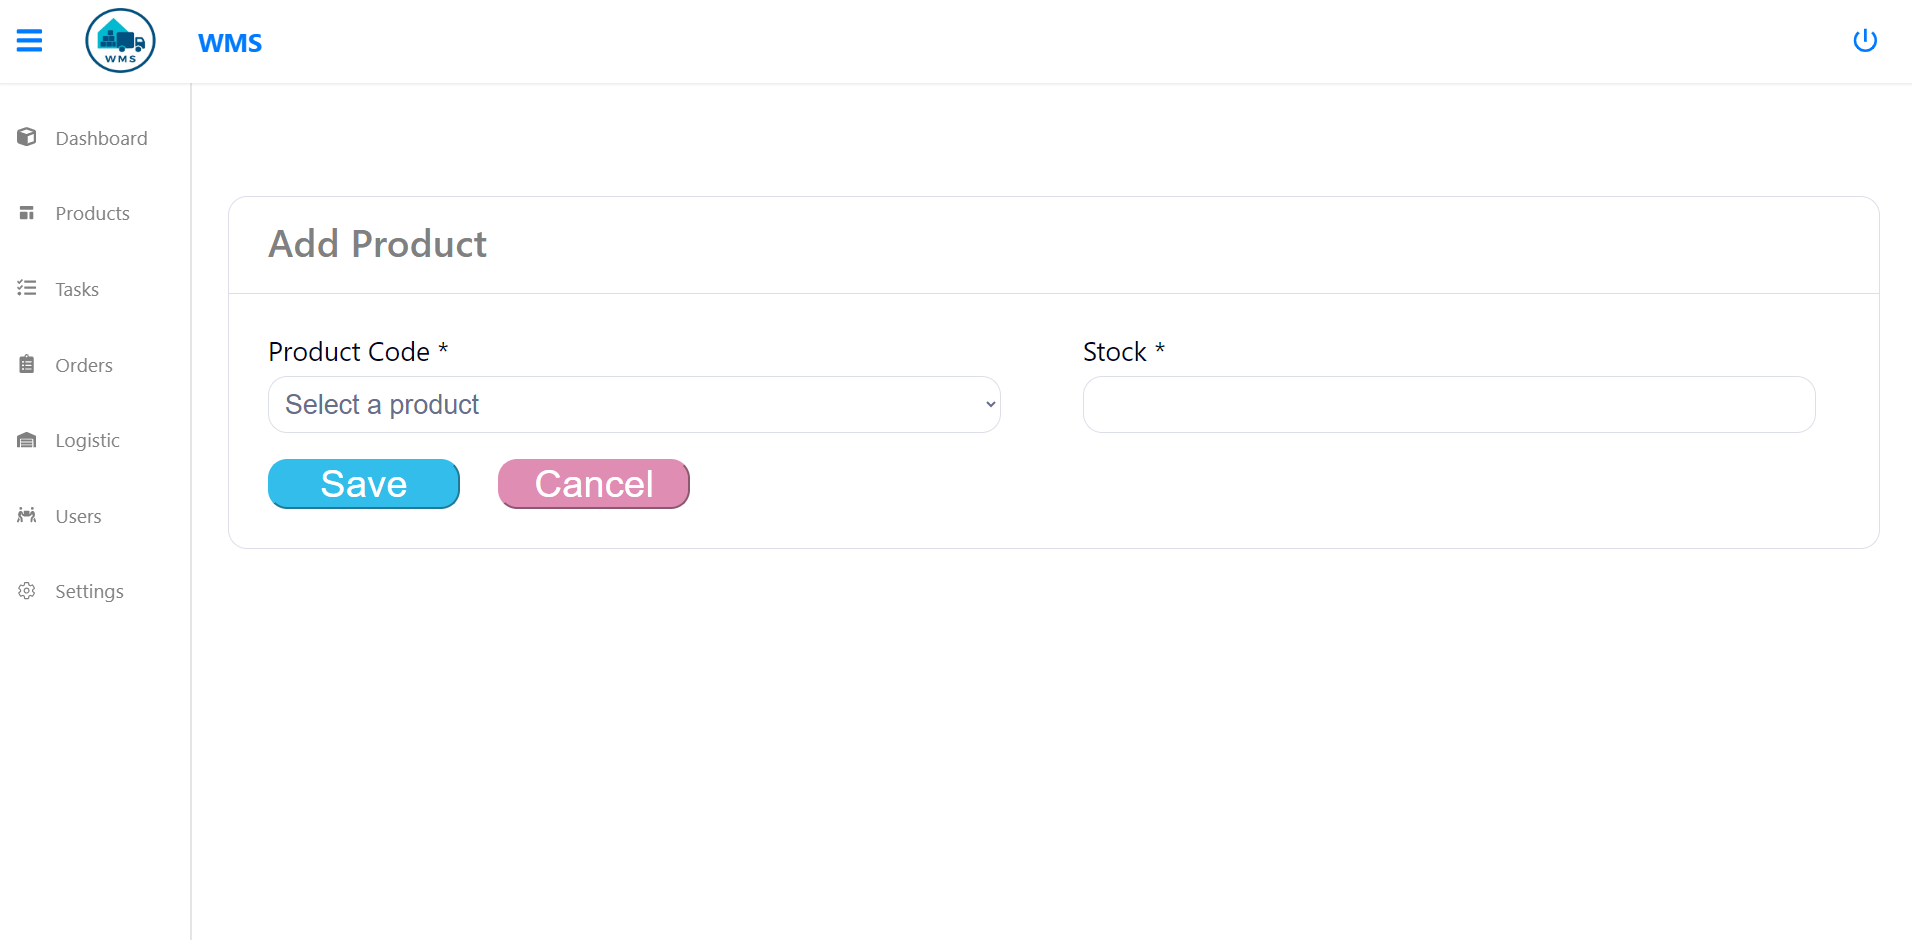
\includegraphics[width=\textwidth]{document/sections/img/Storyboard/addProductInShelf.png}
    \caption{Add Product In Shelf Page}
    \label{fig:addProductInShelfPage}
\end{figure}

Cliccando sul pulsante \textbf{Add Product} nella shelf page si apre un form, che consente
all'Admin di poter aggiungere un nuovo prodotto allo scaffale, specificando il suo codice e la quantità.\\
In basso, sono presenti i pulsanti \textbf{Save} per salvare il prodotto e \textbf{Cancel} per annullare l'operazione
e tornare alla shelf page.\\
Qualora non venissero inseriti correttamente tutti i dati verrà mostrato un messaggio di errore.

\begin{figure}[H]
    \centering
    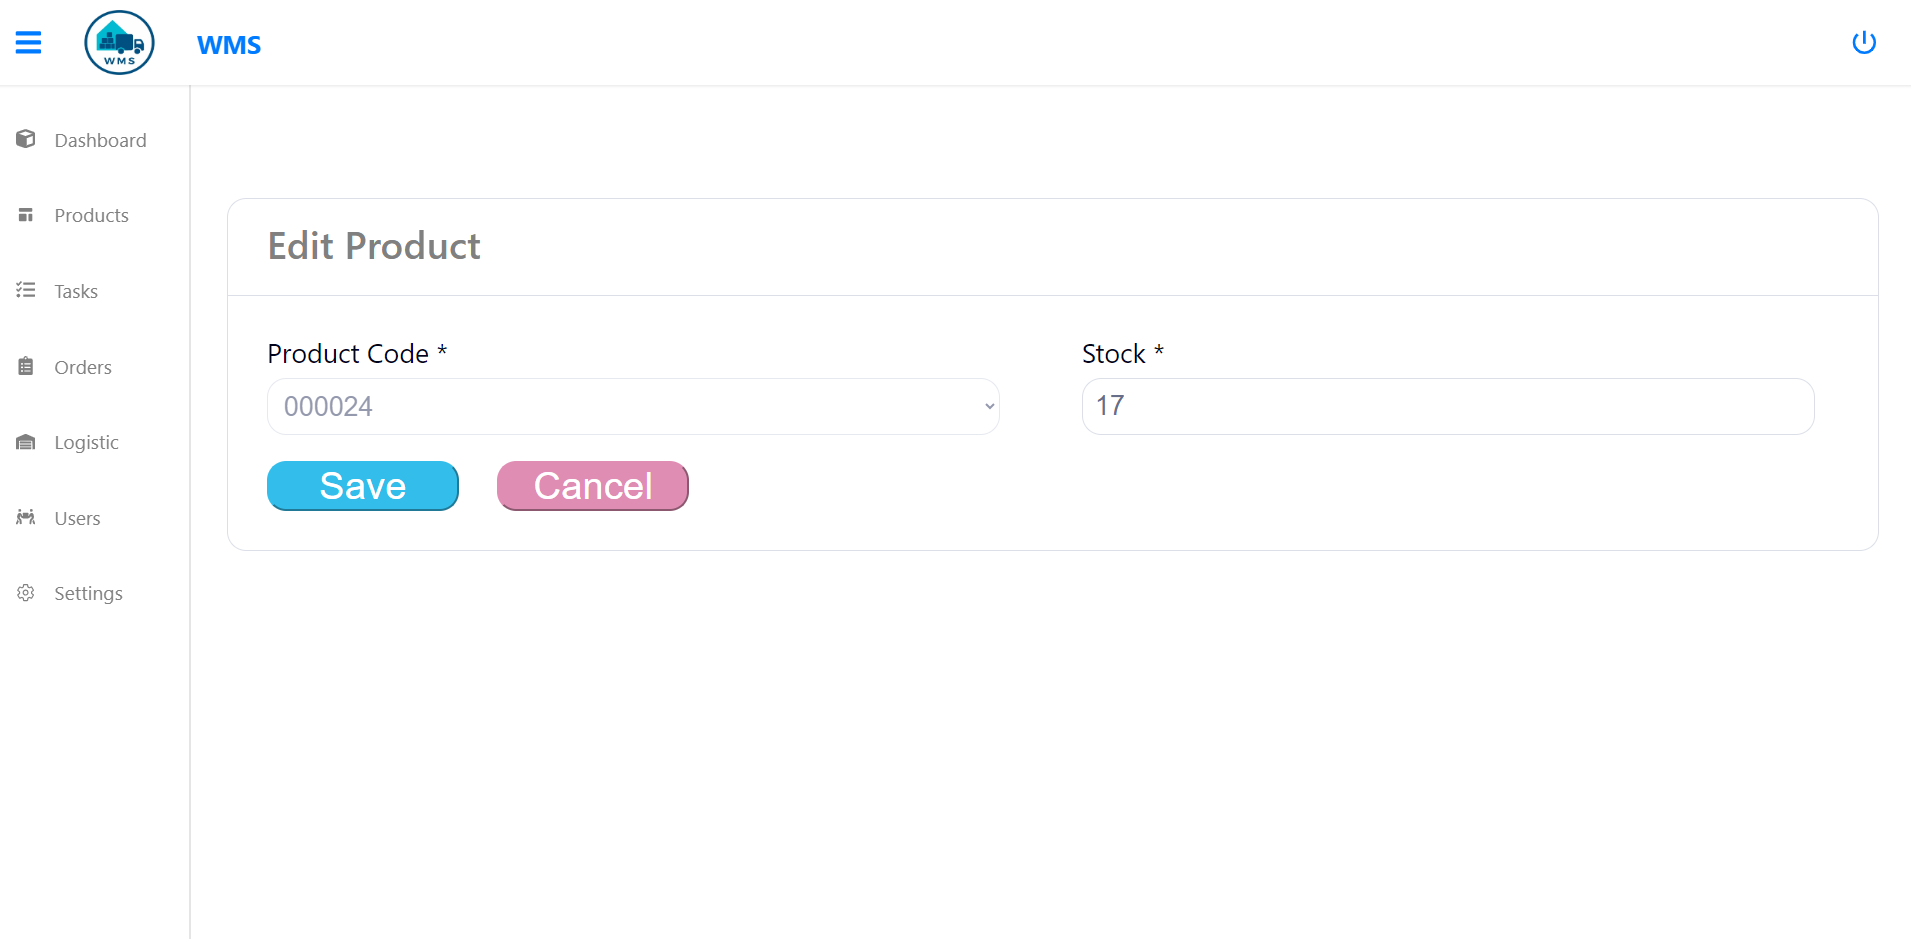
\includegraphics[width=\textwidth]{document/sections/img/Storyboard/editProductInShelf.png}
    \caption{Edit Product In Shelf Page}
    \label{fig:editProductInShelfPage}
\end{figure}

Cliccando sull'icona \textbf{edit} di un determinato prodotto, nella shelf page, si apre un form
che permette all'Admin di modificarne la quantità.\\
Cliccando sul bottone \textbf{Save} vengono salvate le modifiche, mentre cliccando sul bottone \textbf{Cancel} si torna alla shelf page.

\begin{figure}[H]
    \centering
    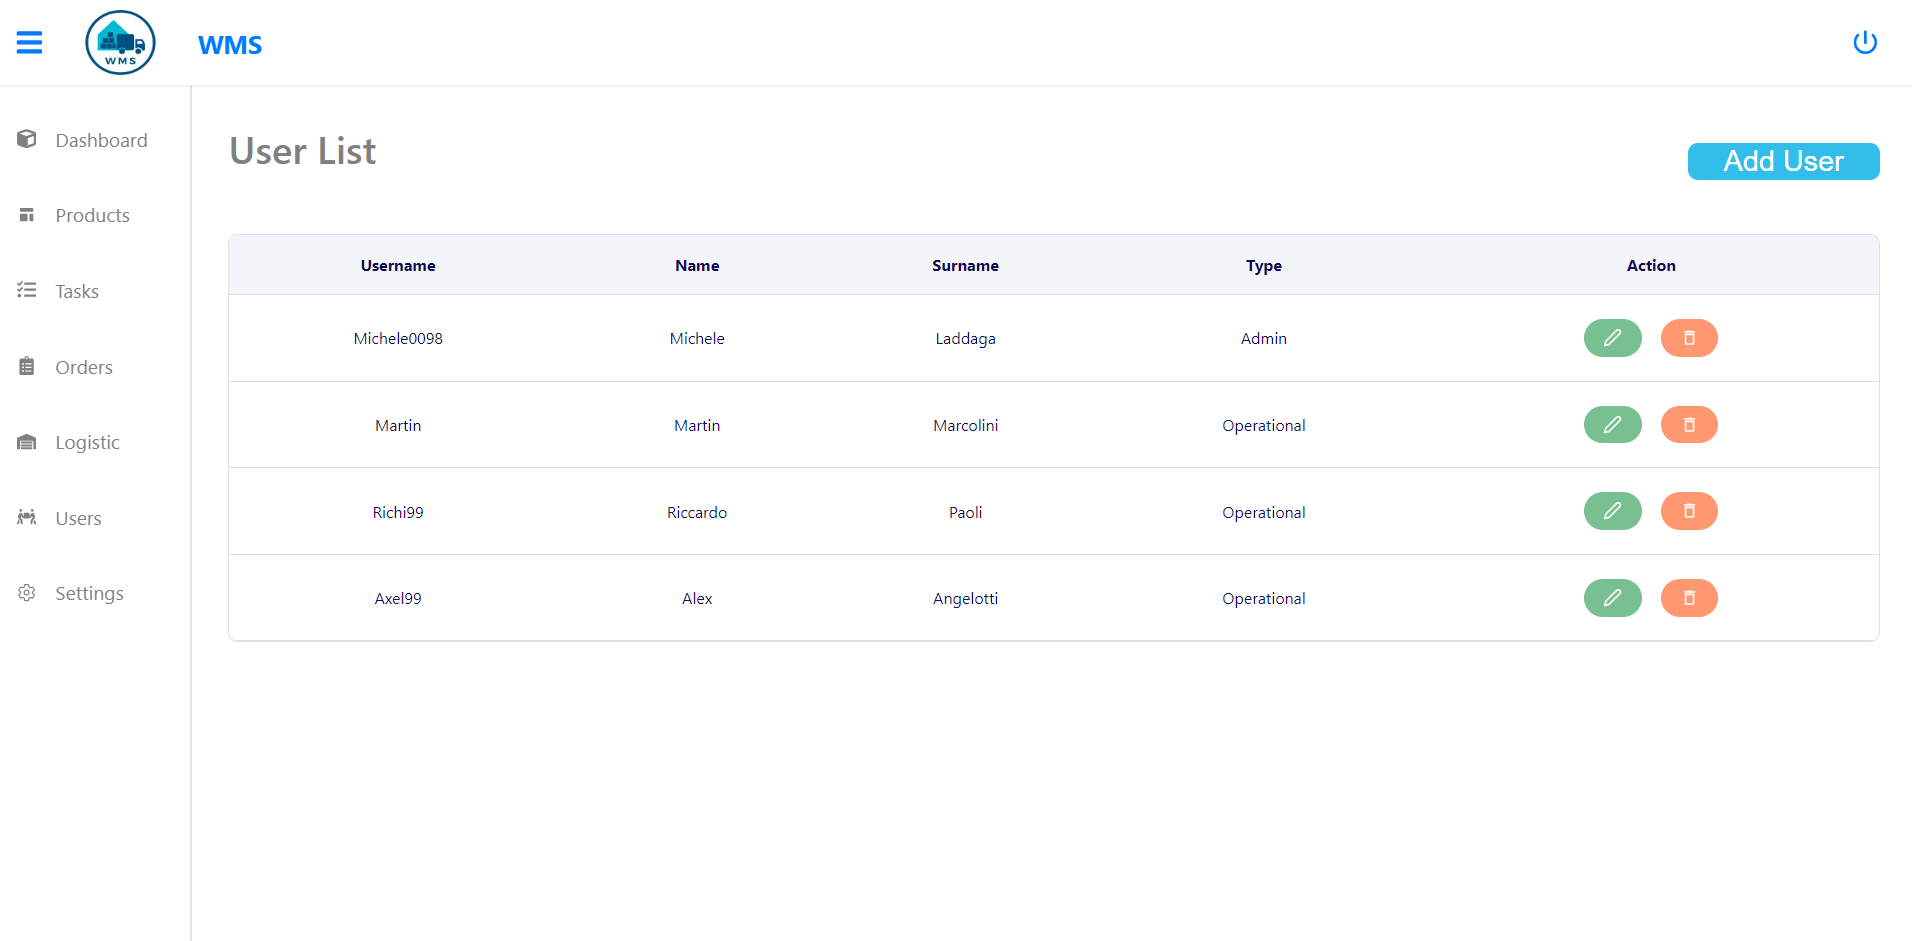
\includegraphics[width=\textwidth]{document/sections/img/Storyboard/usersPage.png}
    \caption{Users Page}
    \label{fig:viewUsersPage}
\end{figure}

Cliccando sulla voce \textbf{Users} nella sidebar, l'utente viene reindirizzato alla pagina di gestione degli utenti.\\
Questa pagina offre una visualizzazione tabellare di tutti gli utenti presenti, sia admin che operational.\\
Nella colonna di destra, sono presenti delle icone che consento di modificare o eliminare
i dati di un singolo utente.\\
In alto a destra è presente un pulsante \textbf{Add Users} che consente di aggiungere un nuovo utente al sistema.

\begin{figure}[H]
    \centering
    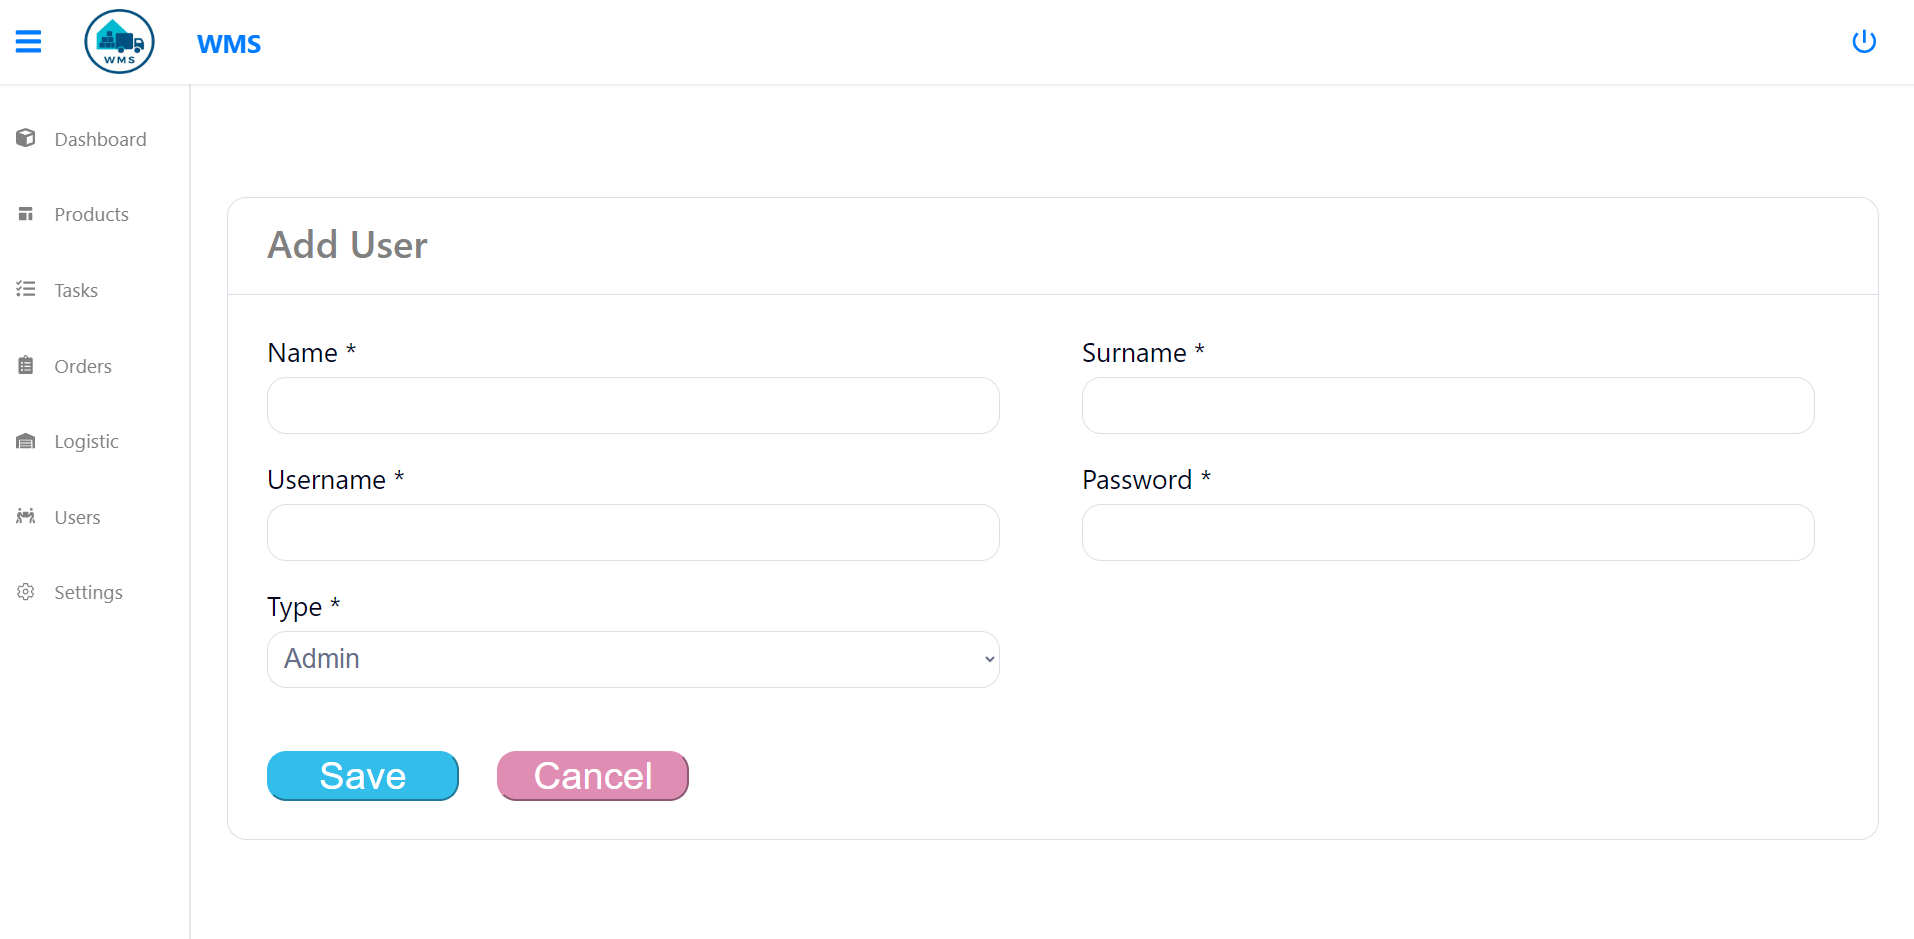
\includegraphics[width=\textwidth]{document/sections/img/Storyboard/addUserPage.png}
    \caption{Add User Page}
    \label{fig:addUserPages}
\end{figure}

Cliccando sul pulsante \textbf{Add User} nella users page si apre un form, che consente
all'Admin di poter creare un nuovo utente specificando tutti i dati richiesti.\\
Infine, in basso, sono presenti i pulsanti \textbf{Save} per salvare l'utente e \textbf{Cancel} per annullare l'operazione
e tornare alla user page.\\
Qualora non venissero inseriti correttamente tutti i dati verrà mostrato un messaggio di errore.

\begin{figure}[H]
    \centering
    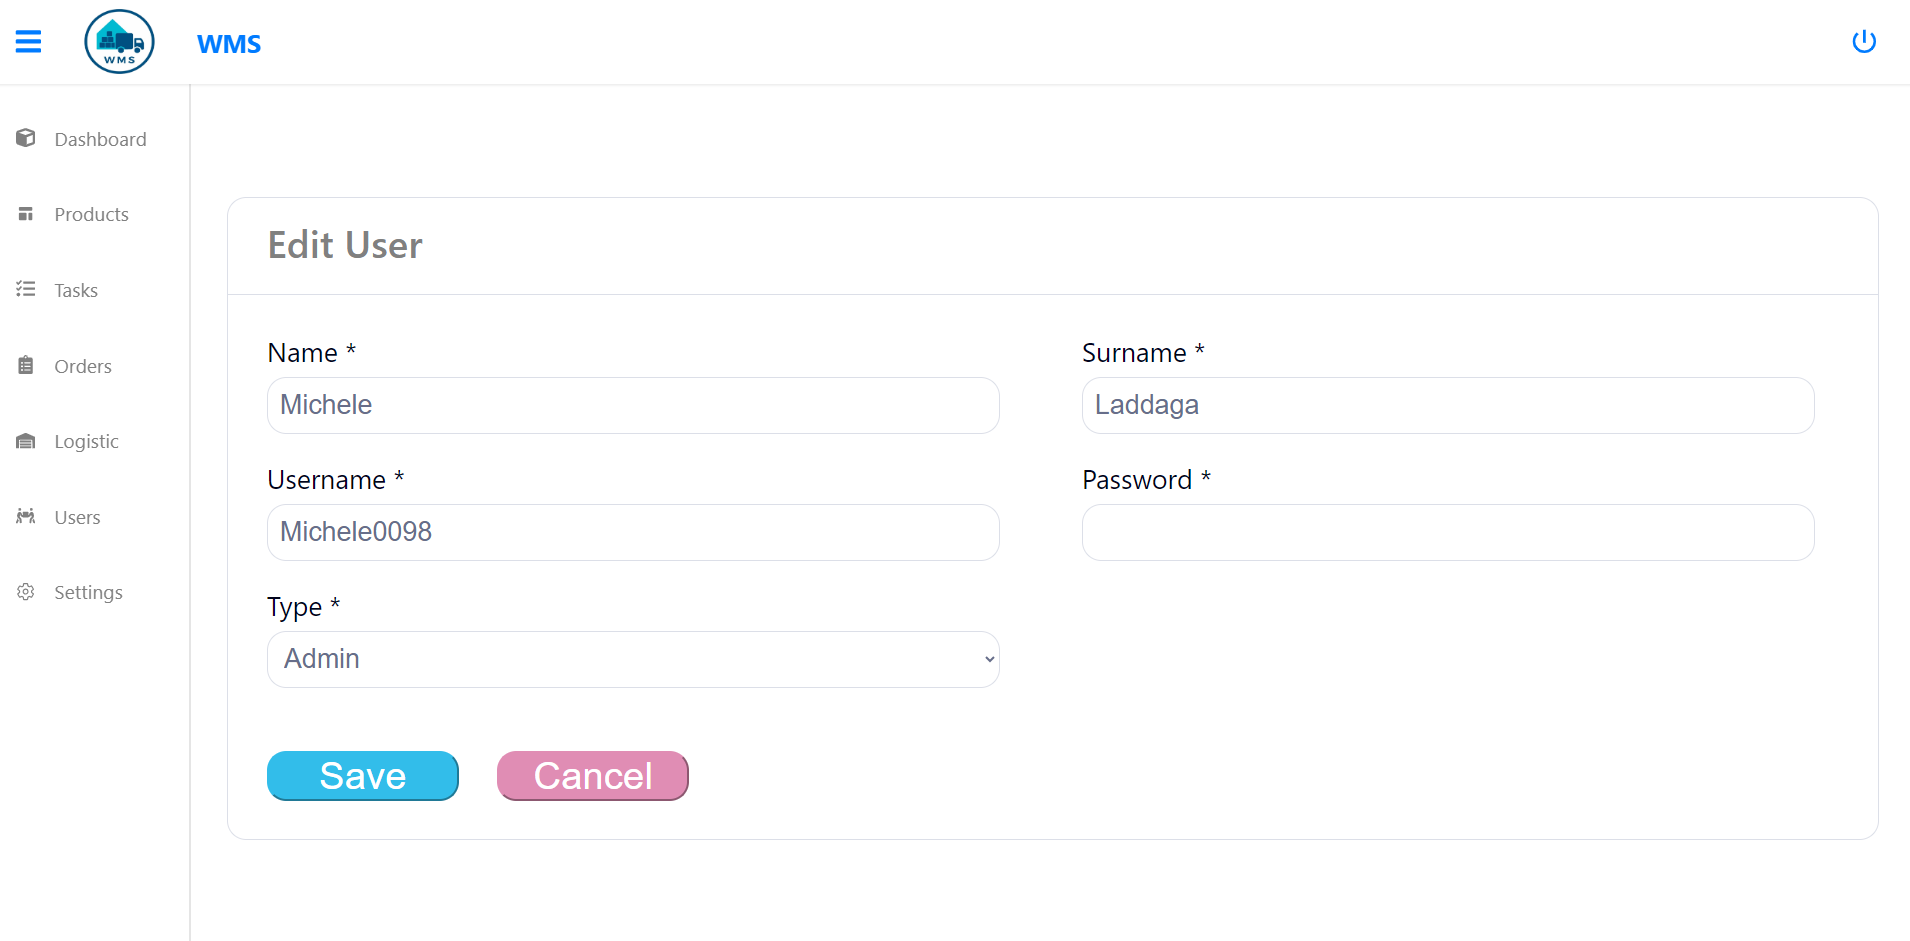
\includegraphics[width=\textwidth]{document/sections/img/Storyboard/editUserPage.png}
    \caption{Edit User Page}
    \label{fig:editUserPage}
\end{figure}

Cliccando sull'icona \textbf{edit} di un determinato utente, nella user page si apre un form simile a quello che
consente di aggiungere un nuovo utente, che permette all'Admin di modificarne i dettagli.\\
Cliccando sul bottone \textbf{Save} vengono salvate le modifiche, mentre cliccando sul bottone \textbf{Cancel} si torna alla user page.

\begin{figure}[H]
    \centering
    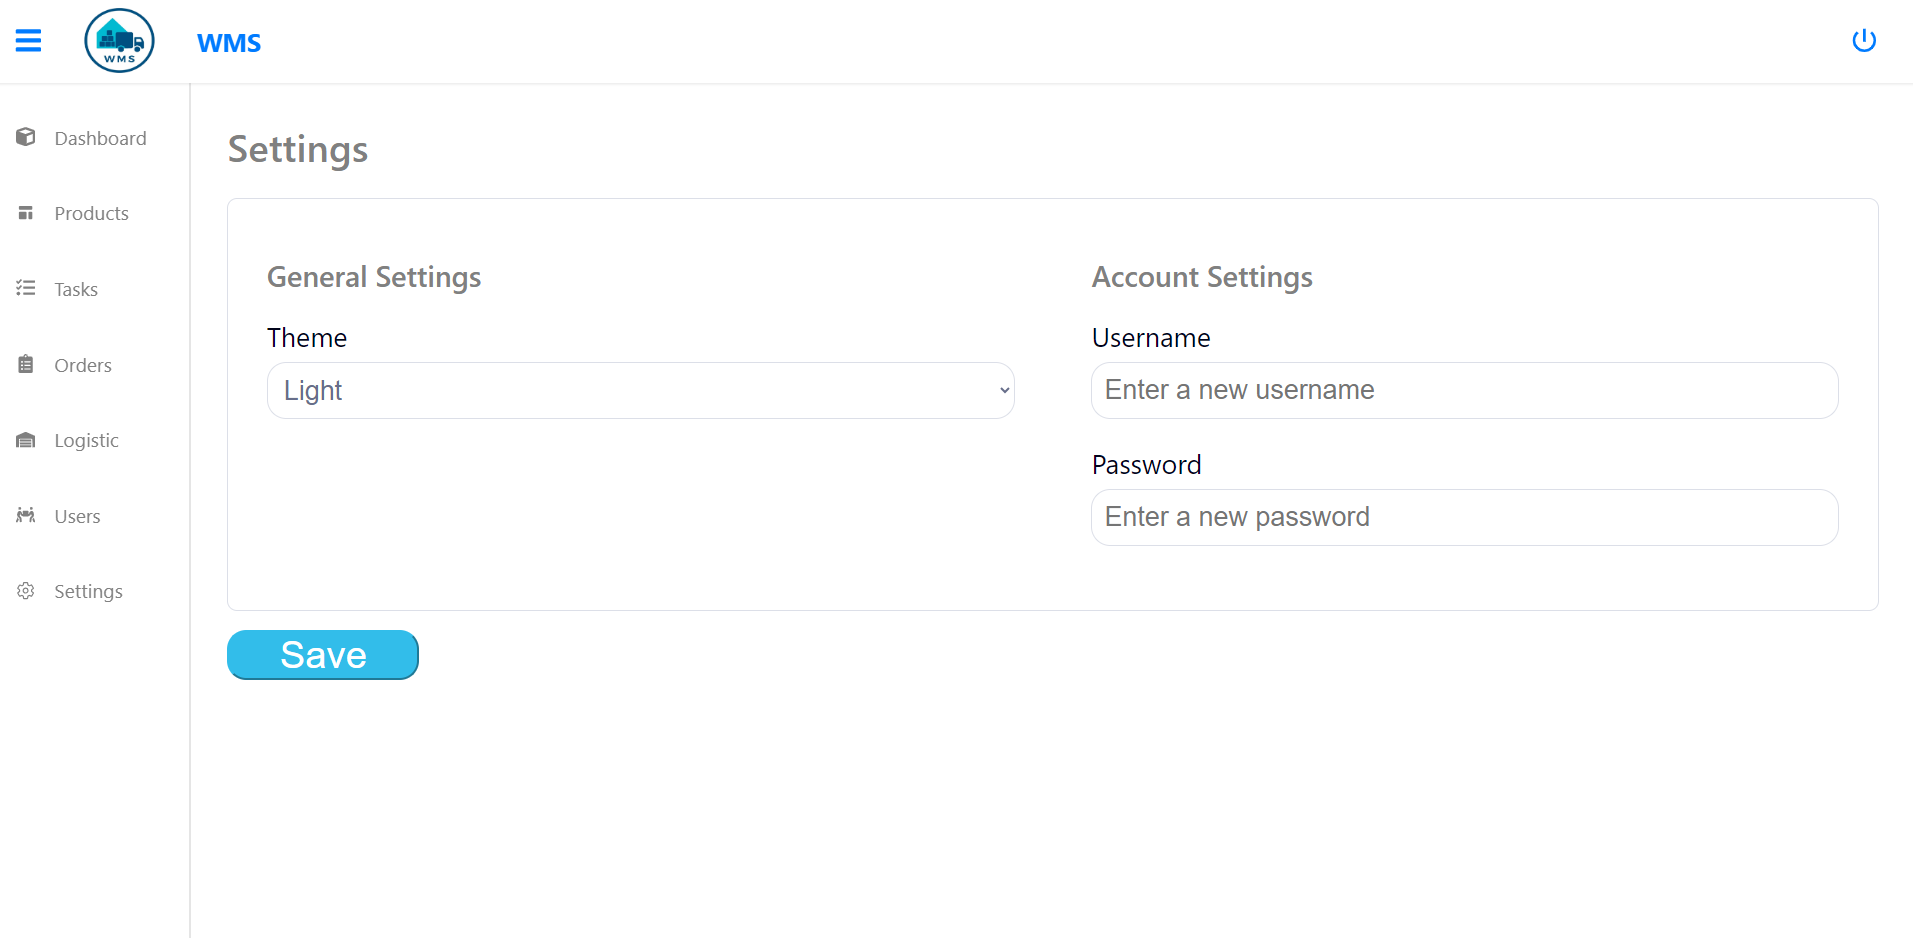
\includegraphics[width=\textwidth]{document/sections/img/Storyboard/settingsPage.png}
    \caption{Settings Page}
    \label{fig:settingsPage}
\end{figure}

Cliccando sulla voce \textbf{Impostazioni} nella sidebar, l’utente viene reindirizzato alla pagina delle impostazioni,
accessibile sia per l'amministratore che per l'utente Operativo.\\
Questa pagina consente di configurare le impostazioni generali, come il tema, e le impostazioni dell'account, come il nome utente e la password.\\
In alto a destra è presente un pulsante \textbf{Save} per salvare le modifiche effettuate.

\subsubsection{Operational}

\begin{figure}[H]
    \centering
    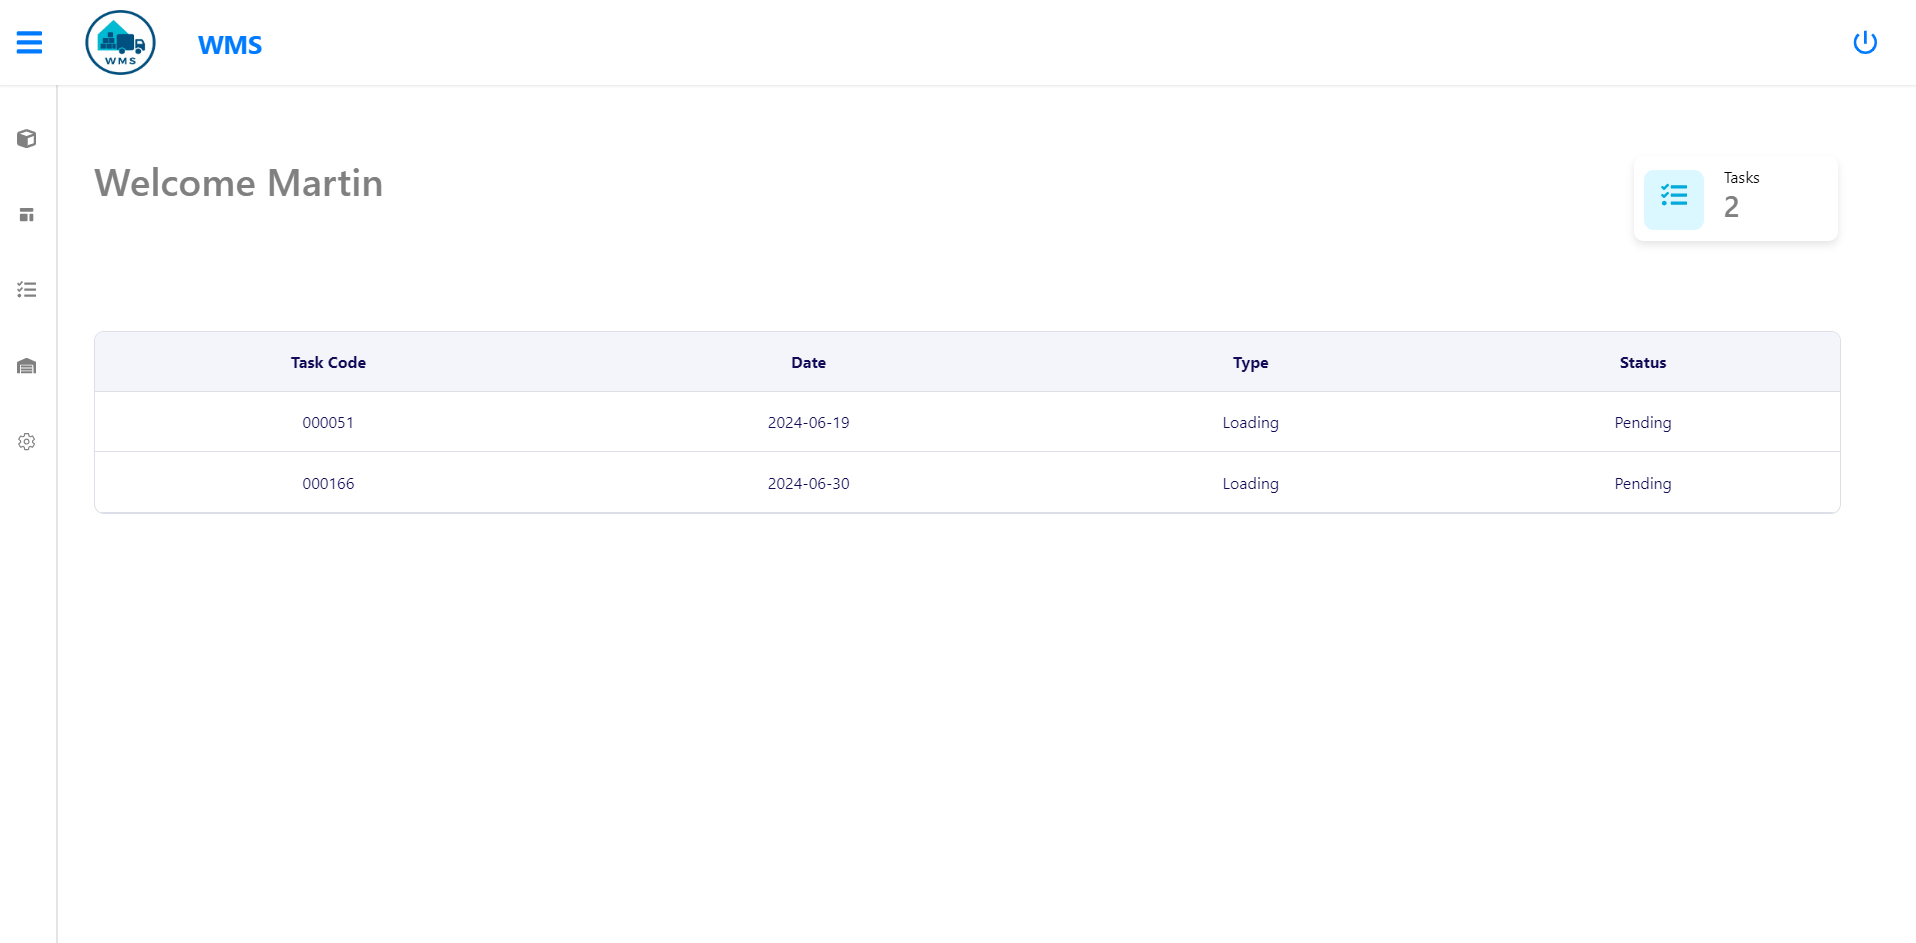
\includegraphics[width=\textwidth]{document/sections/img/Storyboard/homePageOp.png}
        \caption{Home Page Operational}
    \label{fig:homePageOp}
\end{figure}

All'accesso, l'utente Operational viene accolto con un messaggio di benvenuto personalizzato e una panoramica dei task assegnati.\\
La pagina mostra un elenco tabellare dei task, non completati, con il rispettivo codice, data, tipo e stato.\\
Sulla destra, è presente un'icona che indica il numero totale di task assegnati all'utente che ancora deve completare.
\\\\
La \textbf{Product Page} e \textbf{Storage page} presentano una struttura analoga a quella già descritta per l'Admin,
con la differenza che l'utente Operational ha solo permessi di visualizzazione.
\\
\begin{figure}[H]
    \centering
    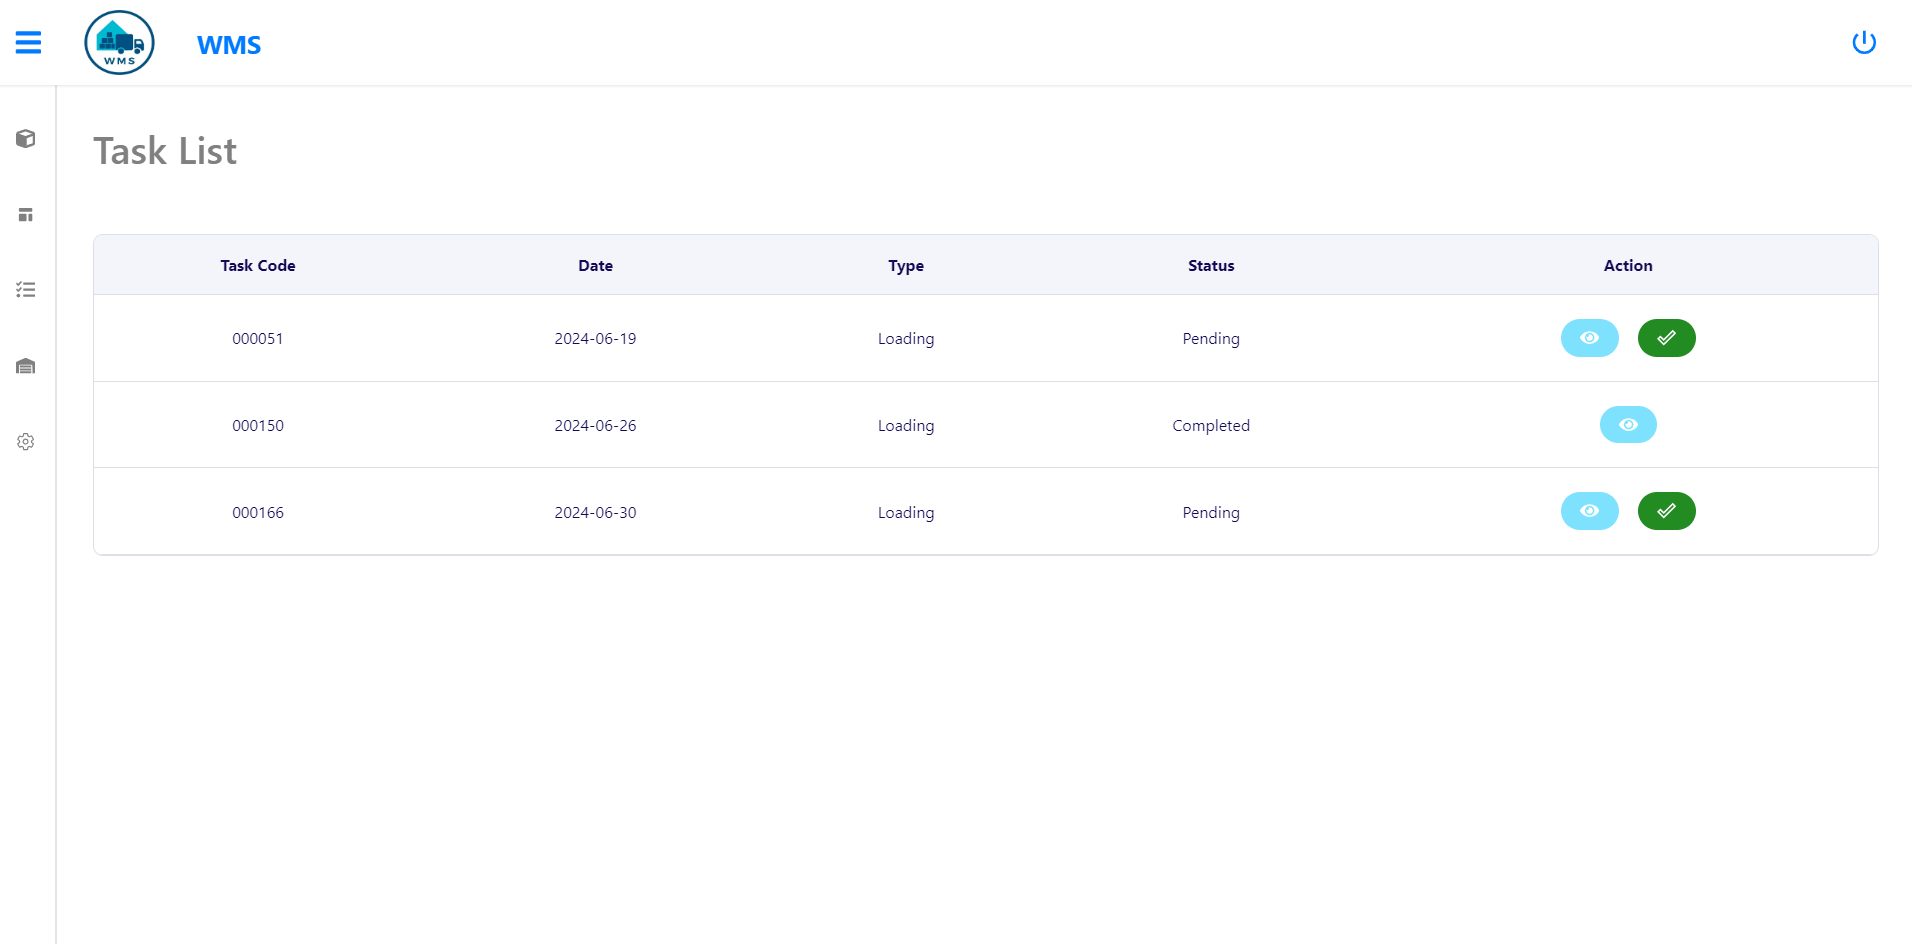
\includegraphics[width=\textwidth]{document/sections/img/Storyboard/userTaskPage.png}
    \caption{User Task Page}
    \label{fig:userTaskPage}
\end{figure}
La \textbf{Task Page} per l'utente Operational ha una struttura simile a quella descritta per l'Admin, ma con alcune
differenze.\\ L'utente Operational non ha la possibilità di eliminare o modificare i dati; può invece consultare i
prodotti da spostare e segnalare il completamento del task cliccando sull'icona \textbf{Done}.